\cleardoublepage
\chapter{Vorgehensmodelle im Softwareengineering}
\label{sec:Kap-2}

\vspace{-1cm}

Wir haben uns in Abschnitt~\ref{sec:Kap-1.2.2} bereits mit dem Softwareentwicklungsprozess und seinen Kernprozessen Anforderungsermittlung/-analyse, Entwurf, Implementierung, Testen, Wartung befasst und dabei sicherlich wenigstens implizit eine gewisse Reihenfolge der Prozesse vermittelt. Auf den ersten Blick erscheint es durchaus naheliegend eine kausale und damit auch zeitliche Abhängigkeit dieser Prozesse untereinander anzunehmen. Es ist zum Beispiel wenig sinnvoll eine Software zu implementieren, von der nicht definiert ist, welche Anforderungen an sie gestellt sind, und es ist nicht möglich Programmcode zu testen, der noch nicht existiert. Daher erscheint es richtig, dass der Prozess der Anforderungsermittlung/-analyse immer vor dem Prozess der Implementierung und Letzterer immer vor dem Prozess des Testens stattfinden muss. Bei genauerem Hinsehen ist die zeitliche Abfolge der Prozesse allerdings weniger eindeutig: So könnte man zum Beispiel die Basisfunktionalitäten einer grafischen Oberfläche implementieren, bevor definiert wurde, welche Buttons und Menüeinträge genau existieren sollen. In diesem Fall würde nur eine sehr allgemein gehaltene Anforderung ("`Es gibt eine grafische Oberfläche"') an das zu erstellende Softwareprodukt definiert, auf deren Grundlage bereits mit der Implementierung begonnen werden könnte. Konkretere Anforderungen könnten später definiert werden. Ähnliches gilt für die Abhängigkeit zwischen Implementierung und Testen: Auch wenn konkreter Programmcode erst dann getestet werden kann, wenn er geschrieben ist, könnten die Testfälle für den zu erstellenden Programmcode durchaus schon vorher spezifiziert werden. Für alle anderen Test- und Qualitätssicherungsmaßnahmen, deren Testgegenstand nicht der reine Programmcode, sondern andere Artefakte des Softwareentwicklungsprozesses sind, gilt dies umso mehr.

\sttpDefinitionskasten{\sttpDefinitionskastenSkalierungsfaktor}{Artefakt}{Das Ergebnis einer Tätigkeit im Softwareentwicklungsprozess.}{Bei Artefakten kann es sich um jegliche Art von Dokumenten oder um Diagramme, formale Spezifikationen, Modelle, einzelne Modell\-ele\-mente, Quellcode oder sonstige Ergebnisse handeln.}

\clearpage %%% für Druck

Wir halten fest, dass zwischen den Kernprozessen des Softwareengineering keine grundsätzlichen zeitlichen Abfolgen bestehen. Abbildung~\ref{fig:prozesse_softwareengineering} zeigt die Kernprozesse des Softwareengineering daher ganz bewusst in einer zufälligen Anordnung. Wie oben aber auch deutlich wurde, existieren auf tieferliegenden Ebenen (Teilprozesse, Aktivitäten, Aufgaben) dagegen sehr wohl Abhängigkeiten. Jedes vernünftige Vorgehen in einem Softwareentwicklungsprojekt wird diese Abhängigkeiten natürlich berücksichtigen.

\begin{figure}[h!]
    \centering
		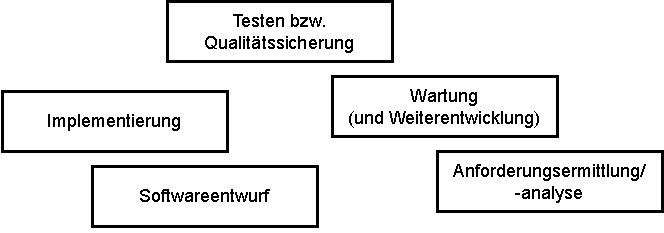
\includegraphics[scale=1.0]{Bilder/Kapitel-2/Abb-2-1.pdf}
    \caption{Kernprozesse des Softwareengineering}
    \label{fig:prozesse_softwareengineering}
\end{figure}

Die Einordnung von Prozessen und Teilprozessen in kausal-zeitliche Abfolgen ist Aufgabe von \textit{Vorgehensmodellen}. 
\marginline{von Prozessen\\zu Vorgehens\-modellen}
Im Rahmen des Softwareengineering beschreiben Vorgehensmodelle, \textbf{wie} der Entwicklungsvorgang von Softwareprodukten ablaufen soll. Je nach Zielrichtung des Vorgehensmodells werden dafür die einzelnen Prozesse und Teilprozesse des Softwareentwicklungsprozesses in bestimmter Reihenfolge und mit bestimmter Schwerpunktsetzung zusammengesetzt, wobei (Teil)Prozese auch wiederholt stattfinden können. Ergebnis ist die Definition eines idealtypisch ablaufenden Softwareentwicklungsprozesses. Für die Entwicklung eines \textbf{konkreten} Softwareprodukts müssen innerhalb des Rahmens des gewählten Vorgehensmodells dann die durchzuführenden konkreten Teilprozesse, Aktivitäten und Aufgaben für die Erstellung des Softwareprodukts bestimmt werden.

% 2.1
\clearpage
\section{Vorgehensmodelle – Ziele und Abgrenzungen}
\label{sec:Kap-2.1}

Die Wahl (und projektspezifische Anpassung) eines Vorgehensmodells gehört als Teil der Projektplanung zu den unterstützenden Prozessen des Softwareengineering und wird dementsprechend in vielen Softwareengineering-Lehrbüchern auch thematisiert. Gleichzeitig findet man Vorgehensmodelle auch in allgemeiner Literatur zum Thema Projektmanagement, da Vorgehensmodelle nicht auf IT-Projekte beschränkt sind.

Vorgehensmodelle stammen ursprünglich aus der Produktionstechnik. Sie unterteilen einen (Produktions)Prozess in logische Abschnitte und definieren zeitliche Abfolgen dieser Prozessabschnitte. Für jeden Prozessabschnitt werden Eintrittsvoraussetzungen, benötigte Ressourcen, durchzuführende Aktivitäten und zu produzierende Ergebnisse (Teilprodukte) festgelegt. Ziel ist es, den Erstellungsprozess eines Produkts so in planbare und kontrollierbare Einheiten zu unterteilen, dass die Erstellung des Produkts mit seinen vorgesehenen Funktionalitäten unter Einhaltung der veranschlagten Zeit- und Kostenbudgets mindestens unterstützt, im Idealfall sogar gesichert wird. Vorgehensmodelle sind in der Regel nicht auf ein einzelnes Produkt ausgerichtet, sondern beschreiben modellhaft abstrahierend und idealisiert Erstellungsprozesse für Kategorien von Produkten. So können (bewährte) Produktionsprozesse wiederholt und auch für andere Produkte übernommen werden.

\minisec{Vorgehensmodelle im Softwareengineering}

Einen idealen Softwareentwicklungsprozess, den man für jede beliebige Softwareentwicklung anwenden könnte, wird es nie geben. Die Menge der durchzuführenden Aufgaben für die Entwicklung eines Softwareprodukts, die Abhängigkeiten und die Reihenfolge dieser Aufgaben und damit auch die Abfolge der sie beinhaltenden (Teil)Prozesse ist spezifisch je nach Softwareentwicklungsprojekt. Vorgehensmodelle können Softwareentwicklungsprozesse jedoch ein Stück weit standardisieren. Sie sind Modelle für die Entwicklung von Softwareprodukten und werden in größerem Maße seit den 1980er Jahren eingesetzt. Sie geben einen (je nach Vorgehensmodell mehr oder weniger flexiblen) Rahmen für die auszuführenden Arbeitsschritte während eines Softwareentwicklungsprozesses vor. Ihr Einsatz soll insbesondere folgende Ziele erfüllen: 
\begin{itemize}
	\item die Komplexitätsreduktion des Softwareentwicklungsprozesses
	\item die Möglichkeit, Softwareprodukte in (großen) Teams zu erstellen
	\item die Sicherstellung von Prozess- und Produktqualität
	\item die strukturierte Steuerung und Kontrolle konkreter Softwareentwicklungsprozesse
	\item die Wiederholbarkeit von (bewährten) Methoden und Vorgehensweisen
	\item die Optimierung bestehender Prozesse bezüglich Zeit, Kosten und Qualität
\end{itemize}

Heute werden im Softwareengineering viele unterschiedliche Vorgehensmodelle eingesetzt. Sie unterscheiden sich unter anderem darin, wie detailliert sie die Abhängigkeiten und Abfolgen der einzelnen (Teil)Prozesse festlegen und in welchem Umfang sie durchzuführende Aufgaben vorgeben, und damit letztlich in der Frage, wie viel Raum sie der Individualität eines konkreten Softwareentwicklungsprozesses geben.

Manche Vorgehensmodelle legen den Fokus auf einzelne Softwareentwicklungsprojekte während andere aus einem höheren Blickwinkel die gesamte Softwareentwicklungsprojekt durchführende Organisation (Firma, Institution) betrachten. Einige Vorgehensmodelle lassen sich auch für beide Ebenen anwenden. In diesem Text betrachten wir nur auf Entwicklungsprojekte bezogene Vorgehensmodelle. Diese werden in der Literatur auch als \textit{Prozessmodelle} bezeichnet. In jüngerer Zeit begegnet einem zudem häufiger auch der Begriff des \textit{Entwicklungsmodells}. Im Englischen werden projektbezogene Vorgehensmodelle mit dem Begriff \textit{Software Life Cycle Model} bezeichnet, 
\marginline{Software-Lebenszyklus}
womit begrifflich der Gegenstandsbereich von Vorgehensmodellen, nämlich der Software-Lebenszyklus, deutlicher wird als in den deutschen Bezeichnungen. Unter einem Software-Lebenszyklus versteht man im engeren Sinne den Prozess von der Erhebung der Anforderungen an die zu erstellende Software bis zur Auslieferung des fertigen Softwareprodukts, im Englischen auch als Software Development Life Cycle (SDLC) bezeichnet. Das Wort Zyklus im Begriff trägt dabei der Tatsache Rechnung, dass auch ein fertiges Softwareprodukt überarbeitet werden und somit der Softwareentwicklungsprozess wieder von vorne beginnen kann. Erweiterte Definitionen ergänzen den SDLC um weitere Prozesse wie zum Beispiel Einsatz, Wartung, Weiterentwicklung und Ausmusterung eines Softwareprodukts, aber auch um Prozesse aus den Bereichen Konfiguration und langfristige Qualitätssicherung zum Software Product Life Cycle (SPLC).

Von Vorgehensmodellen zu unterscheiden sind \textit{Qualitätsmodelle} und \textit{Reifegrad-
	\linebreak %%% für Druck
	modelle}, was aufgrund mancher Überschneidung aber nicht immer konsequent möglich ist. Für Informationen zu einem bestimmten Vorgehensmodell lohnt es sich daher auch in Literaturkapiteln zu Qualitäts- und Reifegradmodellen nachzuschlagen, vielleicht hat die jeweilige Autorin/ der jeweilige Autor das entsprechende Vorgehensmodell dort verortet. Qualitätsmodelle 
\marginline{Qualitäts\-modelle}
bestimmen Qualitätsmerkmale und geben für diese Merkmale Qualitätskriterien und Maßsysteme vor, mit denen die Qualität von Softwareprodukten oder von Softwareentwicklungsprozessen bewertet werden kann. Viele Vorgehensmodelle beinhalten selber keine expliziten Vorgaben zu Qualitätssicherungsmaßnahmen. Konkrete Softwareentwicklungsprojekte, die nach solchen Vorgehensmodellen arbeiten, verwenden daher meist zusätzlich Qualitätsmodelle als Referenz für die Sicherstellung der Qualität ihrer Software oder ihres Entwicklungsprozesses.

Reifegradmodelle (engl. software process assessment model) 
\marginline{Reifegrad\-modelle}
bemessen die Fähigkeit einer Organisation (Softwareentwicklungs)Projekte durchzuführen. Sie tragen ihren Namen aufgrund der von ihnen definierten sogenannten Reifegradstufen, auf denen sich eine Organisation befinden kann. Der Reifegrad sagt aus, wie stark Softwareentwicklungsprozesse in der Organisation schon institutionalisiert sind. Dazu sind jeder Reifegradstufe eine Menge von Anforderungen zugeordnet, die eine Organisation erfüllen muss, um die entsprechende Reifegradstufe zu erreichen. Beispiele für Reifegradmodelle sind CMMI und SPICE\footnote{CMMI: Capability Maturity Model Integration; SPICE: Software Process Improvement and Capability Determination. Für eine Einführung in diese beiden Modelle siehe \cite[565-590]{bal08}. Zu Reifegradmodellen im Allgemeinen siehe \cite[Kap. 8]{swe14} und \cite{sha11}.}. Reifegradmodelle werden wir nicht behandeln.

\pagebreak %%% für Druck

Aufgrund der Unterschiedlichkeit 
\marginline{Vorgehens\-modelle legen strukturierte Verfahren fest} % dieser Absatz
der im Softwareengineering eingesetzten Vorgehensmodelle lässt sich nicht allgemeingültig aufzählen, welche Elemente Vorgehensmodelle genau enthalten und welche Vorgaben sie machen. Allen Vorgehensmodellen gemeinsam ist, dass sie strukturierte Verfahren für die Entwicklung von Softwareprodukten festlegen. So können Reihenfolgen von Prozessen vorgegeben, zu erstellende Artefakte des Entwicklungsprozesses festgelegt und Abfolgen durchzuführender Arbeitsschritte bestimmt werden. Je nach konkretem Vorgehensmodell kann es zusätzlich zum Beispiel Festlegungen zu benötigten Rollen und Kompetenzen, anzuwendenden Methoden oder einzusetzenden Entwicklungswerkzeugen geben. In anderen Vorgehensmodellen drückt sich strukturiertes Verfahren statt durch die Vorgabe von Prozessreihenfolgen dagegen eher durch die Vorgabe grundsätzlicherer Leitlinien und Prinzipien (\zb „den Auftraggeber institutionalisiert ins Projekt einbinden“, „nur lauffähigen Code einchecken“, „gemeinsames Code-Eigentum“) und fester Kommunikationsformate aus.

% 2.2
\clearpage
\section{Kategorien von Vorgehensmodellen}
\label{sec:Kap-2.2}

Konkrete Vorgehensmodelle unterscheiden sich mindestens darin, in welcher Granularität sie die durchzuführenden Tätigkeiten in einem Software\-entwicklungs\-projekt vorgeben. Doch deutlich stärkere Unterschiede zwischen Vorgehensmodellen finden sich, wenn diese unterschiedlichen \textit{Paradigmen} folgen.
\marginline{Paradigma}
Ein Paradigma ist eine grundsätzliche Denkweise/Lehrmeinung, man findet als Synonyme auch die Begriffe Weltanschauung oder Weltbild. Möglicherweise ist Ihnen der Begriff des Paradigmas in der Informatik aus dem Bereich der Programmierung bekannt. Programmier\-sprachen folgen einem Programmierparadigma -- wie zum Beispiel dem objekt-
\linebreak %%% für Druck
orientierten Paradigma --, wenn sie bestimmte im Paradigma festgelegte \mbox{Prinzipien} einhalten.

\begin{figure}[h!]
	\centering
	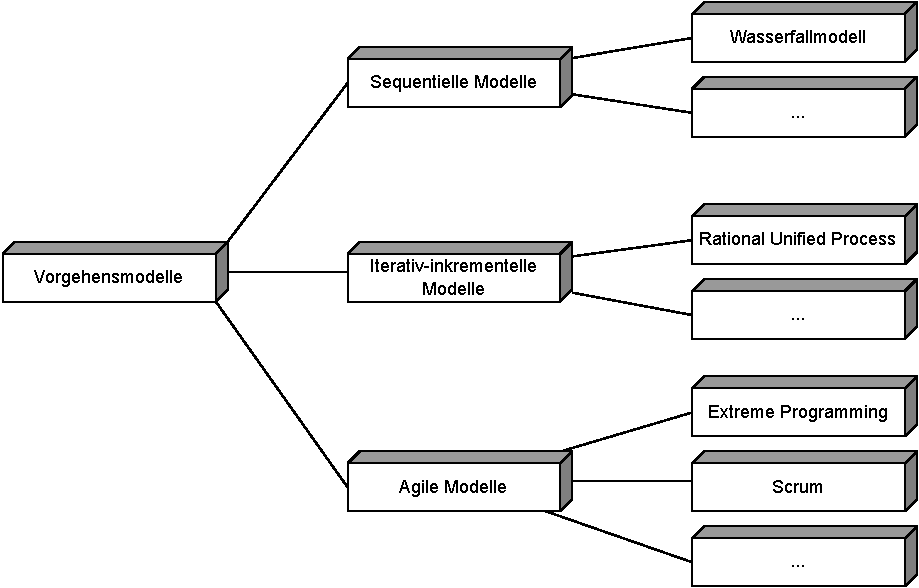
\includegraphics[scale=0.9]{Bilder/Kapitel-2/vorgehensmodelle.pdf}
	\caption{Kategorien von Vorgehensmodellen}
	\label{fig:vorgehensmodelle_komplett}
\end{figure}

Die ersten im Softwareengineering eingesetzten Vorgehensmodelle folgten einem Paradigma, das man als \textit{plangesteuert} bezeichnet. Diesem plangesteuerten Paradigma liegt die Einschätzung zugrunde, dass Softwareentwicklungsprojekte nur dann erfolgreich abgeschlossen werden können, wenn die durchzuführenden (Teil)Prozesse des Softwareengineering und ihr kausal-zeitlicher Ablauf im Vorfeld des Projekts systematisch geplant werden und spätere (Teil)Prozesse immer erst bei Vorliegen von vollständigen, qualitätsgesicherten und dokumentierten Ergebnissen vorhergehender Prozesse starten. Vorgehensmodelle, die dem plangesteuertem Paradigma folgen, gehören zur Kategorie der sogenannten \textit{sequentiellen Modelle} 
\marginline{sequentielle Modelle} 
oder Phasenmodelle. Der bekannteste Repräsentant sequentieller Modelle ist das Wasserfallmodell.

Im Unterschied zum plangesteuerten Paradigma wird im sogenannten agilen Paradigma, das seit Ende der 1990er Jahre verstärkt propagiert wird, die Einschätzung vertreten, dass ein Softwareentwicklungsprojekt nur dann erfolgreich abgeschlossen werden kann, wenn im Projektverlauf Änderungen zugelassen werden können, im Besonderen Änderungen der Anforderungen, und schon ab frühen Zeitpunkten im Projektverlauf lauffähiger (aber auch wieder änderbarer) Programmcode erzeugt wird. Vorgehensmodelle, die dem agilen Paradigma folgen, nennt man 
\marginline{agile Modelle} 
\textit{agile Modelle}. Bekannte Repräsentanten sind Extreme Programming und Scrum.

Sowohl sequentielle als auch agile Modelle werden heute im Softwareengineering eingesetzt. Konkrete Vorgehensmodelle – sowohl diejenigen, die wir in diesem Text vorstellen als auch die vielen anderen, die wir hier nicht thematisieren – passen in der Regel nicht hundertprozentig in genau eine Kategorie, da sie zusätzlich oft auch Kennzeichen anderer Kategorien aufweisen. In der Praxis gilt dies umso mehr, je stärker die Grundform eines Vorgehensmodell individuell an unternehmensspezifische Belange angepasst wird.

Wir werden in den folgenden Abschnitten sowohl allgemeiner die Kennzeichen sequentieller Modelle (Kap.~\ref{sec:Kap-2.2.1}) und agiler Modelle (Kap.~\ref{sec:Kap-2.2.3}) als auch konkrete Vorgehensmodelle als Repräsentanten dieser Kategorien von Vorgehensmodellen vorstellen. Abschnitt~\ref{sec:Kap-2.2.2} thematisiert zwischen der Vorstellung der sequentiellen und der Vorstellung der agilen Modelle eine dritte Kategorie von Vorgehensmodellen, die \textit{inkrementellen und iterativen Modelle}, 
\marginline{inkrementelle und iterative Modelle}
die in den späten 1980er und frühen 1990er Jahren erstmalig vorgestellt wurden und damit auch in ihrer Entstehungszeit zwischen den sequentiellen und den agilen Modellen liegen. Deren zugrundeliegendes Paradigma betont den Stellenwert der fachlichen Aspekte (Strukturen, Geschäftsprozesse etc.) des Einsatzgebiets des zu entwickelnden Softwareprodukts – und kritisiert damit auch die in der Regel sehr technisch orientierte Sichtweise von sequentiellen Vorgehensmodellen. Zum anderen beinhaltet es die Einschätzung, dass für erfolgreich durchzuführende Softwareentwicklungsprojekte lauffähiger Programmcode nicht erst am Ende des Projekts vorliegen darf – hier wurde die Basis für die Programmcode-Fokussierung der späteren agilen Modelle gelegt. 

\minisec{Unterscheidungsmerkmale zwischen Vorgehensmodellen}

Sequentielle, iterativ-inkrementelle (synonym: inkrementell-iterativ) und agile Vorgehensmodelle unterscheiden sich vor allem in folgenden Aspekten, die wir bei der Vorstellung der drei Kategorien in den folgenden Abschnitten jeweils im Detail betrachten werden:

\begin{enumerate}
	\item In welcher Weise werden die einzelnen (Teil)Prozesse zum Softwareentwicklungsprozess zusammengestellt?
	\item Wie wird mit neuen oder veränderten Anforderungen während der Entwicklung umgegangen?
	\item Inwieweit werden Auftraggeber und zukünftige Nutzer des zu erstellenden Softwareprodukts in die Entwicklung einbezogen?
	\item Zu welchen Zeitpunkten liegen auslieferungsfähige Produkte bzw. Teilprodukte vor?
	\item Welche Formen von Artefakten (\zb Programmcode, Dokumente, Modelle) entstehen im Laufe des Softwareentwicklungsprozesses?
\end{enumerate}

\subsection{Sequentielle Modelle}
\label{sec:Kap-2.2.1}

\vspace{\baselineskip} %%% für Druck

\sttpLeserfuehrung{Bilder/Kapitel-2/Leserfuehrung/vorgehensmodelle_sequentiell_illustration.pdf}{Bilder/Kapitel-2/Leserfuehrung/vorgehensmodelle_sequentiell.pdf}

\sttpHervorhebung{\textbf{Sequentielle Vorgehensmodelle}}
\marginline{Entwicklungs\-prozess}
\sttpHervorhebung{\textbf{unterteilen die Softwareentwicklung in aufeinanderfolgende zeitliche Abschnitte (Phasen)}}. 
Dafür werden zunächst die Tätigkeiten, die zur Entwicklung eines auslieferbaren Softwareprodukts notwendig sind, zu Prozessen zusammengefasst (\zb Prozess der Anforderungsanalyse, Prozess der Implementierung). Jedem Prozess entspricht dann eine Phase des sequen\-tiel\-len Vorgehensmodells. Es wird festgelegt, in welcher Reihenfolge die Phasen nacheinander durchlaufen werden. Zudem werden für jede Phase Start- und Endpunkt geplant, die zu erreichenden Ergebnisse definiert, die auszuführenden Tätigkeiten zur Erreichung dieser Ergebnisse spezifiziert, notwendige Input- und Output-Dokumente bestimmt sowie die durchzuführenden Qualitätssicherungs- und Controllingmaßnahmen festgelegt. 

Sequentielle Vorgehensmodelle sehen eine starke Aufgabenteilung vor. So sind einige Mitarbeiter für die Planung des Softwareentwicklungsprojekts, andere für die Implementierung und wieder andere für das Testen des fertigen Softwareprodukts zuständig. Die in einer Phase als Ergebnis produzierten Artefakte werden somit häufig von \textbf{anderen} Mitarbeitern in folgenden Phasen weiterverarbeitet. Sie müssen dementsprechend vollständig und verständlich sein. Eine Phase in einem sequen\-tiel\-len Vorgehensmodell kann erst beginnen, wenn die vorhergehende Phase komplett abgeschlossen wurde, was in der Regel durch das Erreichen von zuvor definierten Meilensteinen ausgedrückt wird. In einem ideal ablaufenden Projekt ist die Kontrolle des Projektfortschritts durch die im Vorfeld terminierten Meilensteine sehr einfach. 

\vspace{\baselineskip} %%% für Druck

\sttpDefinitionskasten{\sttpDefinitionskastenSkalierungsfaktor}{Meilenstein}{Ein überprüfbares Zwischenziel innerhalb eines Projekts.}{Meilensteine werden zu Beginn eines Projekts definiert und zeitlich festgelegt. Im Laufe des Projekts kann anhand der erreichten und noch nicht erreichten Meilensteine der Projektfortschritt und der ggf. bestehende Zeitverzug im Projekt bestimmt werden. Der Begriff Meilenstein stammt aus dem klassischen Projektmanagement.}

\vspace{\baselineskip} %%% für Druck

Die strenge Form des sequentiellen Vorgehensmodells sieht vor, dass jede Phase nur genau einmal durchlaufen wird, die Phasen überschneidungsfrei sind und dementsprechend auch niemals in eine bereits abgeschlossene Phase zurückgekehrt werden kann. Dem liegt die idealisierte Vorstellung zugrunde, dass jede Phase fehlerfrei abgearbeitet werden kann und auf dieser optimalen Basis dann die folgende Phase beginnen kann. In der Praxis trifft das selten zu. Die Vorgabe, jede Phase nur einmal zu durchlaufen, würde zum Beispiel bedeuten, auch dann nicht in eine Entwurfs\-phase zurückkehren zu können, wenn Fehler oder Unvollständigkeiten des Entwurfs erst während der Implementierung auffallen. Man müsste auf Grundlage des fehlerhaften oder unvollständigen Entwurfs weiterarbeiten – wodurch das entstehende Softwareprodukt nicht (alles) das tut, was es tun soll –, oder bei der Implementierung ganz bewusst vom vorliegenden Entwurf abweichen. Letzteres würde implizit Entwurfsaktivitäten in die Phase der Implementierung verlagern, was dem Charakter eines sequentiellen Vorgehensmodells widerspricht, weil es das Konzept der inhaltlich abgegrenzten Phasen unterläuft. Die in der Praxis eingesetzten sequen\-tiel\-len Vorgehensmodelle sehen fast immer iterative Elemente vor. So kann zumindest in die zuvor abgeschlossene Phase zurückgekehrt werden, sofern Fehler, Unvollständigkeiten oder Unklarheiten bestehen. Die entsprechende Phase wird somit erneut durchlaufen und die Ergebnisse der Phase werden entsprechend angepasst. Abbildung~\ref{fig:prozesse_softwareengineering_sequentiell} zeigt Prozesse des Softwareengineering in einer sequentiellen Abfolge.

\begin{figure}[h!]
    \centering
		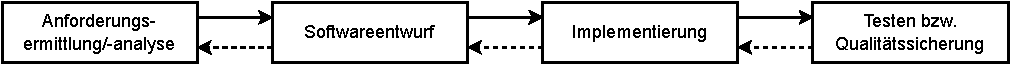
\includegraphics[width=1.0\textwidth]{Bilder/Kapitel-2/Abb-2-3.pdf}
    \caption[Prozesse des Softwareengineering in sequentieller Abfolge]{Prozesse des Softwareengineering in der sequentiellen Abfolge Anforderungsermittlung-Entwurf-Implementierung-Testen. Die gestrichelten Pfeile stellen die Rückkehrmöglichkeiten in die jeweils vorhergehende Phase dar.}
    \label{fig:prozesse_softwareengineering_sequentiell}
\end{figure}

\sttpHervorhebung{\textbf{Sequentielle Vorgehensmodelle}} 
\marginline{Umgang mit Anforderungen} 
\sttpHervorhebung{\textbf{definieren sämtliche Anforderungen zu Projektbeginn.}}
Dieser Katalog an Anforderungen bildet bei Auftragsarbeiten in der Regel auch die inhaltliche Grundlage für den Vertragsabschluss zwischen dem Auftraggeber und der Firma oder Institution, die die Softwareentwicklung übernimmt. Änderungen und Ergänzungen in Bezug auf die Anforderungen sind überhaupt nur dann möglich, wenn im Vorfeld zwischen Auftraggeber und Auftragnehmer (rechtlich) eindeutige Änderungsprozesse – vor allem in Bezug auf die Kostenübernahme – definiert wurden. Die sequentiellen Modelle eignen sich daher am besten für Projekte, deren Anforderungen von Anfang an vollständig und präzise definiert sind und in denen die Anforderungen auch über die Projektlaufzeit stabil bleiben. Implizit setzen sequentielle Vorgehensmodelle zudem voraus, dass das Softwareentwicklungsteam über einen erfahrenen Projektleiter verfügt, der anhand der Anforderungen eine realistische Abschätzung bezüglich Zeitaufwand und Kosten der Entwicklung vornehmen kann.

\sttpDefinitionskasten{\sttpDefinitionskastenSkalierungsfaktor}{Projektleiter}{Diejenige Rolle, die für ein konkretes Softwareentwicklungsprojekt organisatorische und koordinierende Aufgaben übernimmt.}{Wir verwenden den Begriff in einem sehr weiten Sinne. Die Person, die die Rolle Projektleiter übernimmt, kann gleichzeitig Personalführungsverantwortlichkeiten besitzen oder selber auch Entwicklungstätigkeiten ausführen oder mehrere Projekte leiten etc. Je nach Unternehmen bzw. Vorgehensmodell kann diese Rolle auch die Bezeichnung Projektmanager, Entwicklungsleiter, Scrum Master etc. tragen.}

\sttpHervorhebung{\textbf{Sequentielle Vorgehensmodelle}} 
\marginline{Einbezug Kunde}
\sttpHervorhebung{\textbf{binden Auftraggeber oder zukünftige Nutzer eher weniger ein.}} 
Auftraggeber und zukünftige Nutzer des Softwareprodukts werden nur zu Beginn des Projekts in den Prozess der Anforderungsermittlung einbezogen. Alle späteren Entwurfs- und Implementierungstätigkeiten sowie auch ein großer Teil der Test\-akti\-vitäten finden nur innerhalb des Entwicklungsteams statt. Dem Auftraggeber wird das Produkt erst am Ende des Projekts zur sogenannten Abnahme – Prüfung, ob das Produkt die vertraglich vereinbarte Leistung erbringt – wieder vorgelegt.

\sttpHervorhebung{\textbf{Sequentielle Vorgehensmodelle}}
\marginline{Artefakte}
\sttpHervorhebung{\textbf{sind dokumentenorientiert.}}
Als Ergebnis einer Phase entstehen ein oder mehrere Dokumente (\zb Pflichtenheft, Entwurfs\-spezifikation, Diagramm der Systemmodule), die Grundlage der nächsten Phase sind und dort weiter verfeinert, ergänzt oder angepasst werden. Eine große Heraus\-forderung besteht darin, diese Dokumente untereinander, aber auch in Bezug auf den endgültigen Programmcode des Softwareprodukts, während des gesamten Entwicklungsprozesses konsistent zu halten.
%\sttpgls{Konsistenz}

\sttpHervorhebung{\textbf{Sequentielle Vorgehensmodelle}} 
\marginline{Auslieferung}
\sttpHervorhebung{\textbf{liefern das Produkt erst mit Ende des Softwareentwicklungsprojekts aus.}} 
Zwar können auch während des Entwicklungsprozesses bereits lauffähige Versionen mit Teilfunktionalität existieren, doch werden diese nicht für den produktiven Einsatz herausgegeben.

Ein bekannter Vertreter sequentieller Vorgehensmodelle ist das Wasserfallmodell. Es ist das erste Vorgehensmodell, das in großem Maße im Softwareengineering eingesetzt wurde.

\clearpage %%% für Druck

\subsubsection{Wasserfallmodell(e)}
\label{sec:Kap-2.2.1.1}

\vspace{\baselineskip} %%% für Druck

\sttpLeserfuehrung{Bilder/Kapitel-2/Leserfuehrung/vorgehensmodelle_sequentiell_illustration.pdf}{Bilder/Kapitel-2/Leserfuehrung/vorgehensmodelle_wasserfall.pdf}

Die Überschrift deutet es schon an: Eigentlich ist es falsch von \textbf{dem} Wasserfallmodell zu sprechen, da es Wasserfallmodelle heute in vielen Varianten gibt. Dementsprechend unterschiedliche Abbildungen findet man in der Literatur.

\minisec{Historische Wasserfallmodelle} 

Das ursprüngliche Wasserfallmodell stellte Winston W. Royce 1970 vor \cite{roy70}. \mbox{Royce} orientierte sich für sein Modell an der Darstellung eines sequentiellen Prozessmodells aus den 1950er Jahren\footnote{Das sogenannte \textit{stagewise model}, ein Prozessmodell für die Systementwicklung des Semi-Automatic Ground Environment Systems (SAGE), das erste computergestützte Luftverteidigungssystem Nordamerikas (USA, Kanada). 1956 von Herbert D. Benington beschrieben \cite{ben56}, zusammenfassend zum Modell \cite[43\psq]{kne17}.}, verdichtete dessen ursprünglich neun Phasen zu sieben, ergänzte sogenannte Rückkopplungsmöglichkeiten (Rückkehr von einer Phase in die vorhergehende Phase) und führte die an einen Wasserfall erinnernde Darstellung ein. Abbildung~\ref{fig:wasserfallmodel_nach_royce} zeigt das Wasserfallmodell von Royce.  

\begin{figure}[h!]
    \centering
    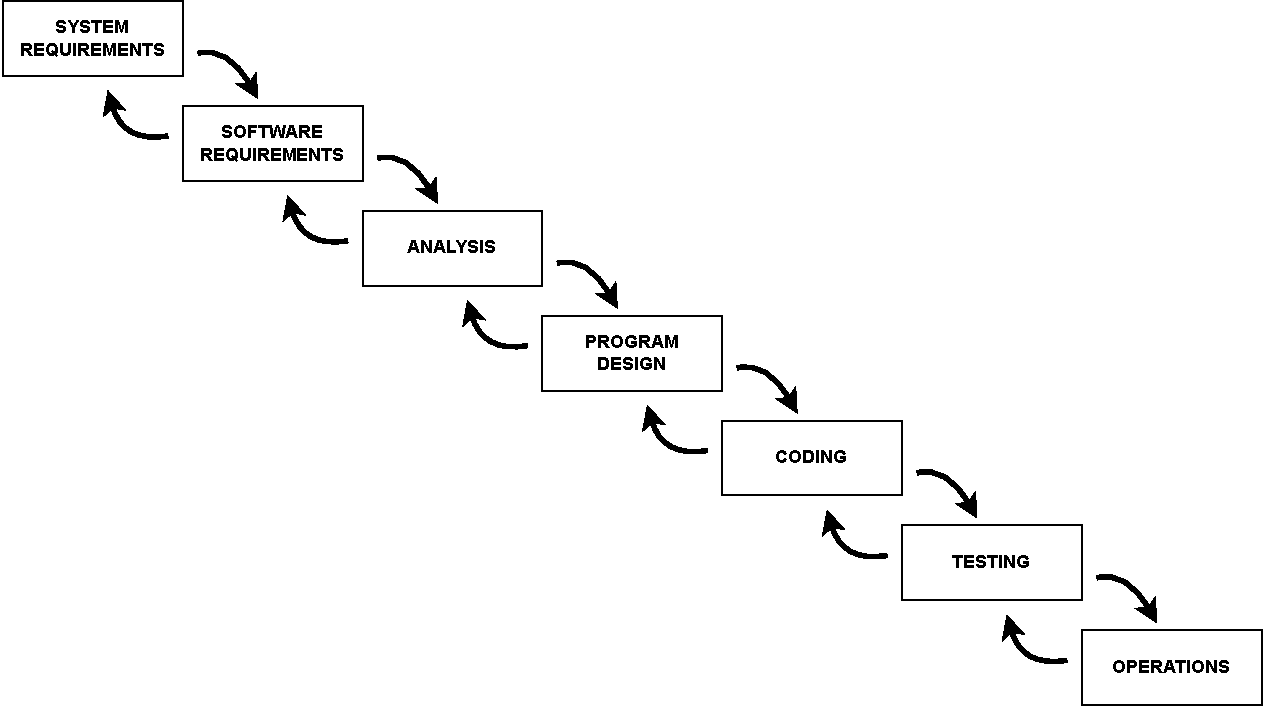
\includegraphics[width=1.0\textwidth]{Bilder/Kapitel-2/WasserfallmodellRoyce.pdf}
    \caption[Wasserfallmodell von Royce]{Wasserfallmodell von Royce, nach \cite[330]{roy70}}
    \label{fig:wasserfallmodel_nach_royce}
\end{figure}

\pagebreak %%% für Druck

In mancher Literatur findet sich die Unterscheidung zwischen einem Wasserfall\-modell \textbf{ohne} und einem Wasserfallmodell \textbf{mit} Rückkehrmöglichkeit in die vorhergehende Phase. Dies ist allerdings ein Irrtum, der darauf zurückzuführen ist, dass der Artikel von Royce zur Hinführung auf sein Modell auch wasserfallartige Abbildungen ohne Rückkehrmöglichkeiten enthält. Das von ihm vorgeschlagene Modell sieht die Rückkopplung zur jeweils vorhergehenden Phase aber explizit vor. Kaum in Erinnerung geblieben ist zudem, dass Royce eng verknüpft mit seinem Modell Maßnahmen zur Reduzierung von Entwicklungsrisiken vorschlägt, die man heute erst später entstandenen Vorgehensmodellen zuordnet. Dazu gehören eine kontinuier\-liche Einbeziehung der zukünftigen Nutzer (in Royce' Modell noch an festen Punkten im Projektablauf) und das Arbeiten mit Prototypen 
%\sttpgls{Prototyp}
(er verwendet den Begriff pilot model).

Vermehrt eingesetzt für die Softwareentwicklung werden Wasserfallmodelle seit den Veröffentlichungen von Barry W. Boehm  in den 1980er Jahren. Abbildung~\ref{fig:wasserfallmodel_nach_boehm} zeigt das Wasserfallmodell von Boehm.  

\begin{figure}[h!]
    \centering
    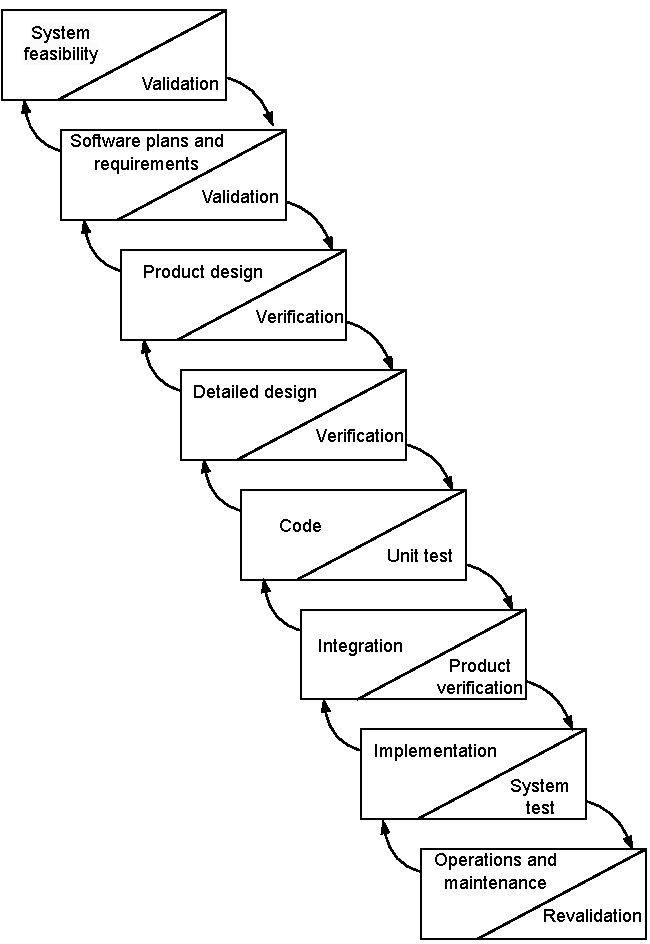
\includegraphics[scale=0.75]{Bilder/Kapitel-2/WasserfallmodellBoehm.pdf}
    \vspace{\baselineskip} %%% für Druck
    \caption[Wasserfallmodell von Boehm]{Wasserfallmodell von Boehm, nach \cite[36]{boe81}}
    \label{fig:wasserfallmodel_nach_boehm}
\end{figure}

\pagebreak %%% für Druck

Boehm erweiterte Anfang der 1980er Jahre das Modell von Royce, indem er den Zuschnitt der einzelnen Phasen veränderte, den Punkt der Softwarewartung (engl. maintenance) ergänzte und Qualitätssicherungsaspekte explizit ins Modell aufnahm. Boehm war zudem derjenige, der den Namen Wasserfallmodel populär machte.

\minisec{Heutige Wasserfallmodelle}

Heute findet man überwiegend fünf- und sechsphasige Wasserfallmodelle. Abbildung~\ref{fig:wasserfallmodel_fuenf_phasen} zeigt links ein beispielhaftes fünfphasiges Wasserfallmodell und rechts ein sechsphasiges. 

\begin{figure}[h!]
    \centering
		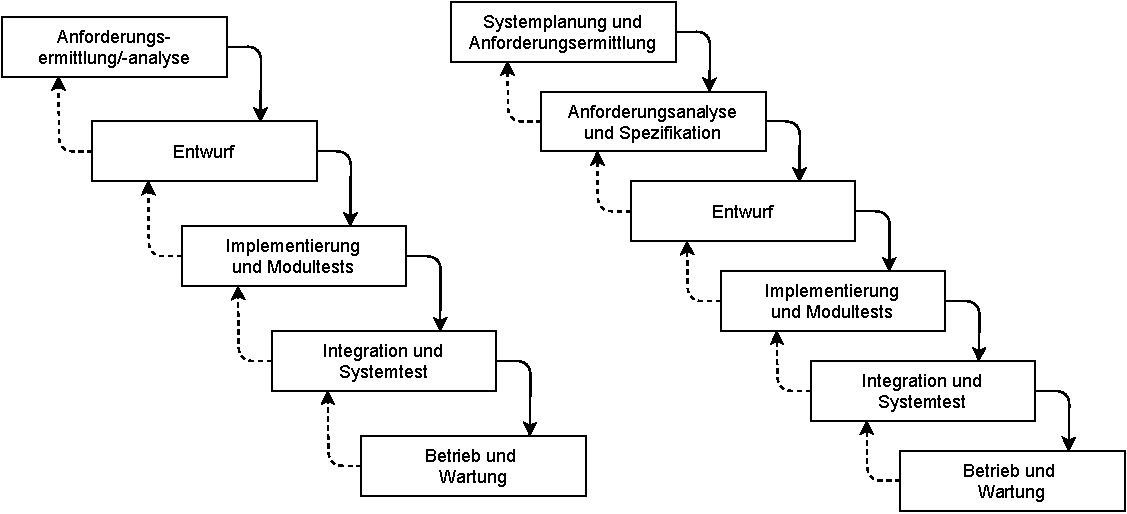
\includegraphics[width=1.0\textwidth]{Bilder/Kapitel-2/Abb-2-6.pdf}%
    \caption{Beispielhaftes fünf- bzw. sechsphasiges Wasserfallmodel}
    \label{fig:wasserfallmodel_fuenf_phasen}
\end{figure}

Im Vergleich zu fünfphasigen werden bei sechsphasigen Wasserfallmodellen meistens explizit Tätigkeiten der Planung des Softwareentwicklungsprojekts (\zb Kalkulation, Projektplan) integriert und der Prozess rund um die Spezifizierung von Anforderungen auf zwei Phasen aufgeteilt. Zum Beispiel sind die Erstellung von Lastenheft 
%\sttpkapitelverweis{Lastenheft und Pflichtenheft}{Kap.~\ref{sec:Kap-6.2.5}}
und Pflichtenheft bei fünfphasigen Modellen üblicherweise beide Teil der ersten Phase, während bei sechsphasigen Modellen die Erstellung des Pflichtenhefts erst zur zweiten Phase gehört. 

Die Wasserfallmodelle in Abbildung~\ref{fig:wasserfallmodel_fuenf_phasen} sind nur beispielhafte Ausprägungen fünf- und sechsphasiger Wasserfallmodelle. Die in konkreten Softwareentwicklungsprojekten eingesetzten Wasserfallmodelle unterscheiden sich von diesen Abbildungen, aber auch untereinander, oftmals im konkreten Zuschnitt und damit auch in der Benennung der einzelnen Phasen. Dies betrifft insbesondere den Bereich des Testens, bezogen auf die Abbildungen damit die Trennung zwischen der Phase Implementierung und Modultests %\sttpgls{Softwaretests} 
und der folgenden Phase Integration und Systemtest. Hier reicht das Spektrum von der kompletten Auslagerung des Testens in die spätere Phase – womit in der Implementierungsphase nur reine „Debugging-Tests“ stattfinden – bis zur Durchführung kompletter Integrationstests in der früheren Phase – womit in der späteren Phase nur noch der Systemtest verbleibt. 

\minisec{Struktur des Softwareentwicklungsprozesses}

\vspace{1.5mm} %%% für Druck

Das Wasserfallmodell ist ein sehr starres sequentielles Vorgehensmodell. Es sieht vor, dass mit einer Phase erst dann begonnen wird, wenn sämtliche Aktivitäten der vorherigen Phase abgeschlossen wurden und die entstandenen Ergebnisse qualitätsgesichert sind – dementsprechend alle Meilensteine erreicht sind. Der zu Beginn des Softwareentwicklungsprozesses einmal festgelegte Ablauf der abzuarbeitenden Aktivitäten wird nach Möglichkeit eingehalten.

\vspace{0.6mm} %%% für Druck

Aus Managementsicht besticht das Wasserfallmodell damit vordergründig durch seine Einfachheit. Anhand von Meilensteinen ist der Projektfortschritt jederzeit kontrollierbar. Zu Beginn eines Projekts kann eine systematische Planung der benötigten Personalressourcen erfolgen. Aufgrund des unterschiedlichen inhaltlichen Zuschnitts der einzelnen Phasen und der umfangreichen Dokumentation der Ergebnisse einer Phase ist es dabei möglich, für verschiedene Phasen unterschiedliche (auch örtlich unverbundene) Teams einzusetzen. Schon zu Beginn des Projekts kann zum Beispiel kalkuliert werden, wann ein erfahrener Softwarearchitekt und wann das Team der Softwaretester benötigt wird. Die abgegrenzten Zuschnitte der Phasen und die Ausrichtung auf zu erreichende Meilensteine führen zudem in der Regel dazu, dass in einem Projekt auch die einzelnen Arbeitsaufgaben innerhalb einer Phase stark vorgegeben sind. Gerade für Softwareentwickler mit wenig Erfahrung kann das Orientieren an festen Vorgaben und das Abarbeiten begrenzter Aufgaben hilfreich sein.

\vspace{0.6mm} %%% für Druck

Auch wenn das Wasserfallmodell die Rückkehr in schon abgeschlossene Phasen vorsieht, hängen Umfang und Anzahl der möglichen Überarbeitungen in der Praxis davon ab, wieviel zeitlicher Puffer für das Projekt eingeplant wurde. Der Einsatz eines Wasserfallmodells erfordert daher einen erfahrenen Projektleiter, der den Projektplan und die einzelnen Arbeitsschritte zielführend und realistisch durchführbar festlegt und dabei im Projektplan auch ausreichende Zyklen (Rückkehr in bereits abgeschlossene Phasen) für eventuell notwendige Überarbeitungen von Ergebnissen vorsieht. 

\vspace{0.6mm} %%% für Druck

In der Praxis ist die vorgesehene Abgeschlossenheit der Phasen zudem nicht immer notwendig, zum Beispiel weil Komponenten des zu entwickelnden Softwareprodukts so unabhängig voneinander sind, dass mit der Implementierung einer Komponente (\zb Benutzerverwaltung) begonnen werden könnte, bevor der Entwurf für eine andere Komponente (\zb Seminarverwaltung) komplett erstellt ist. Außerdem  treten in den meisten Projekten Verzögerungen im Projektablauf ein, sei es weil Mitarbeiter ausfallen, Aufwände für Tätigkeiten falsch eingeschätzt wurden oder Fehler bemerkt werden, die zeitaufwändig korrigiert werden müssen. Die geringe Flexibilität des Wasserfallmodells macht es schwierig auf solche Risikofaktoren zu reagieren. Sofern der Auslieferungstermin der Software nicht verschoben werden kann, führen Verzögerungen im Projektablauf oft zur Verkürzung der späteren Phasen des Projekts. Da im Wasserfallmodell der Bereich des Testens die letzte Phase vor der Auslieferung der Software bildet, gehen solche Verzögerungen in der Regel zu Lasten der Testaktivitäten.

\vspace{0.6mm} %%% für Druck

Hinzu kommt, dass durch die späte Testphase 
\marginline{späte Testphase}
Fehler sowie unvollständige oder unklare Spezifikationen erst spät im Projektverlauf offensichtlich werden. Spät erkannte Fehler sind oft teurer als frühzeitig erkannte Fehler, da größere Personalressourcen für Arbeiten auf fehlerhafter Grundlage investiert wurden. Sollten beim Testen oder auch erst im Betrieb noch größere Fehler in der Software entdeckt werden, ist es zudem zu spät Grundlegendes zu ändern. Es bleiben dann nur noch provisorische Behelfslösungen (engl. Workarounds), die die Symptome des fehlerhaften Verhaltens der Software behandeln, aber nicht die grundlegenden Probleme lösen. Um solche Situationen zu vermeiden, sehen viele heutige Wasserfallmodelle schon parallel zur Implementierung Testaktivitäten vor (\zb Tests einzelner Komponenten). Der abschließende sogenannte Systemtest, bei dem die Software gegen alle spezifizierten Anforderungen getestet wird, findet in Wasserfallmodellen in der Regel aber weiterhin erst in der letzten Phase vor der Auslieferung statt. Sollte dabei das Fehlen von Funktionalitäten bemerkt werden, ist es in den meisten Fällen zu spät, daran etwas zu ändern.

\minisec{Umgang mit Anforderungen}

Die Anforderungen an das zu erstellende Softwareprodukt werden im Wasserfall\-modell ganz zu Beginn des Softwareentwicklungsprojekts ermittelt. Sobald die Anforderungsspezifikation 
%\sttpkapitelverweis{Anforderungsspezifikation}{Kap.~\ref{sec:Kap-6.1.x}} 
erstellt und (vom Auftraggeber) geprüft wurde, können in der Regel keine neuen oder veränderten Anforderungen berücksichtigt werden. Das ist ein Problem: Zwischen der Planung eines Softwareentwicklungsprojekts und der Auslieferung des fertigen Produkts können durchaus mehrere Jahre liegen. In dieser Zeit können sich Arbeitsprozesse sowie Erfahrungen und Erwartungen von Nutzern schon derart verändert haben, dass das entwickelte Produkt die Bedürfnisse seiner Nutzer schon zum Zeitpunkt seines Ersteinsatzes nicht mehr erfüllt. Hinzu kommt, dass es nur selten wirklich möglich ist die Anforderungen zu Projektbeginn hundertprozentig vollständig und unmissverständlich zu erfassen.

\vspace{2mm}

\sttpDefinitionskasten{\sttpDefinitionskastenSkalierungsfaktor}{Kunde}{Auftraggeber oder Nutzer des Softwareprodukts.}{Wir verwenden den Begriff Kunde als Verallgemeinerung in Kontexten, in denen eine Unterscheidung zwischen Auftrag\-geber auf der einen Seite und Nutzer auf der anderen Seite nicht sinnvoll bzw. möglich ist.}

\minisec{Einbezug des Kunden}

Die Einbindung des Auftraggebers oder zukünftiger Nutzer des Softwareprodukts in den Prozess der Softwareentwicklung ist nur in der Zeit der Anforderungsermittlung/
\linebreak %%% für Druck
-analyse vorgesehen. In der Praxis kommt es natürlich trotzdem vor, dass auch in späteren Phasen bei Unklarheiten mit dem Auftraggeber Rücksprache gehalten wird, eine systematische Rücksprache in der Entwurfsphase (oder sogar in der Implementierungsphase) sieht das Wasserfallmodell aber nicht vor. Das kann auch bei im Projektverlauf stabilen Anforderungen leicht dazu führen, dass die wirklichen Vorstellungen der Kunden im fertigen Produkt unzureichend umgesetzt sind.

Wichtig für die erfolgreiche Softwareentwicklung mit einem Wasserfallmodell ist, dass im Softwareentwicklungsteam eine sehr genaue Kenntnis des fachlichen Problembereichs vorliegt, um die fehlende Einbindung und das somit nicht vorhandene Feedback des Kunden kompensieren zu können.

\vspace{2mm} %%% für Druck

\minisec{Artefakte des Entwicklungsprozesses}

Als sequentielles Vorgehensmodell ist das Wasserfallmodell dokumentenorientiert. Ein Großteil der Tätigkeiten während des Softwareentwicklungsprozesses ist darauf ausgerichtet, verschiedene Dokumente
\marginline{Dokumente}
zu erstellen (\zb Anforderungsspezifikation, Architekturspezifikation, Komponentenmodell, Testplan). Die Meilensteine am Ende der Phasen beziehen sich dementsprechend auch meistens auf das Vorliegen bestimmter Dokumente, welche dann in der Regel die Basis für die Aktivitäten der folgenden Phase bilden. Aufgrund dieser dokumentenorientierten Ausrichtung entsteht während der Entwicklung des Softwareprodukts eine umfangreiche technische Dokumentation des Systems. Dies erleichtert die Einarbeitung neuer Mitarbeiter während des Projekts, aber auch die Einarbeitung derjenigen Mitarbeiter, die das erstellte Softwaresystem später betreiben sollen.

\vspace{2mm} %%% für Druck

\minisec{Einsatz von Wasserfallmodellen}

Trotz aller Kritikpunkte am Wasserfallmodell sollte man seine Bedeutung nicht geringschätzen. Zum einen hat das Wasserfallmodell viel dazu beigetragen, unter Softwareentwicklern ein Verständnis für die notwendige Trennung zwischen den fachlichen Anforderungen auf der einen Seite und ihrer technischen Umsetzung auf der anderen Seite zu etablieren. Zum anderen haben sich auf Basis des Wasserfallmodells und insbesondere auch anhand seiner Probleme andere Arten von Vorgehensmodellen herausgebildet, die es ohne die – schon in den 1980er Jahren geführte – intensive Diskussion über die Vor- und Nachteile des Wasserfallmodells vielleicht nicht geben würde.

In  der Literatur finden sich unterschiedliche Ansichten darüber, in welchen Situationen und für welche Institutionen und Projekte es auch heute noch sinnvoll ist, ein Wasserfallmodell als Vorgehensmodell zu verwenden. Als typische
\marginline{Anwendungs\-bereiche}
Anwendungs\-bereiche werden oft eingebettete Systeme (engl. embedded systems) und sicherheitskritische Systeme genannt. Bei eingebetteten Systemen übernimmt die Software die Steuerung der Hardware sowie die Interaktion mit der Außenwelt. Da sich die Hardware nicht verändern lässt, sobald sie produziert wurde, müssen die Aufgaben\-teilung zwischen Hardware und Software und damit die genauen Anforderungen an die Software zu Beginn der Entwicklung festgelegt werden. Genauso orientiert sich der Entwurf der Software an den Gegebenheiten der Hardware. Da ein eingebettetes System aufgrund der Inflexibilität der Hardware damit in der Regel sowieso schwer auf veränderte Anforderungen reagieren kann, steht dieser Aspekt auch für die entsprechende Softwareentwicklung nicht so sehr im Vordergrund. Für die Entwicklung sicherheitskritischer Systeme gilt eine Reihe von Vorschriften, die bei der Softwareentwicklung eingehalten werden müssen. Dazu gehören oft auch formale Analysen von Spezifikations- und Entwurfsdokumenten, die nachweisen sollen, dass die notwendigen sicherheitskritischen Anforderungen berücksichtigt sind. Da es sich dabei um einen aufwändigen und teuren Prozess handelt, der idealerweise nur einmalig im Laufe der Entwicklung des Softwareprodukts stattfindet, sollten die Entwurfs\-tätig\-keiten vollständig abgeschlossen sein, bevor die formalen Analysen durchgeführt werden. Aber auch wenn in Projekten für eingebettete oder sicherheitskritische Systeme vielleicht häufiger Wasserfallmodelle zu finden sind, bedeutet das nicht, dass dort andere Vorgehensmodelle gar nicht eingesetzt würden. Auf der anderen Seite kann man auch in anderen Anwendungsgebieten auf wasserfallartige Vorgehensmodelle treffen.

In der Praxis wird die Entscheidung für ein Vorgehensmodell 
\marginline{Entscheidung für ein Vorgehens\-modell}
häufig nicht aufgrund der expliziten Abwägung seiner Vor- und Nachteile gegenüber den Vor- und Nachteilen anderer Vorgehensmodelle getroffen werden, sondern aufgrund weicherer Faktoren: Ein Unternehmen, das mit einem Wasserfallmodell erfolgreich ein Produkt für einen Kunden entwickelt hat, wird bei einem ähnlichen Produkt für einen anderen Kunden vermutlich wieder ein Wasserfallmodell wählen. Ein Projektleiter, der bei seinem letzten Projekt die Einbindung des Kunden schmerzlich vermisst hat, wird versuchen diesen Aspekt im neuen Projekt zu verbessern und damit evtl. auch zu einem anderen Vorgehensmodell wechseln. Wasserfallmodelle (oder andere Arten von sequentiellen Modellen) werden seit über vierzig Jahren in Soft\-ware\-entwick\-lungs\-projekten eingesetzt. Viele Unternehmen, die Software für interne oder externe Zwecke entwickeln, haben daher Arbeitsprozesse in anderen Abteilungen als der Softwareentwicklungsabteilung auf solche Vorgehensmodelle ausgerichtet (\zb die Bereiche Auftragsaquise, Vertragswesen, Personalplanung, Controlling). Gerade der Umstieg von einem sequentiellen Wasserfallmodell auf agile Vorgehensmodelle erfordert oft auch Veränderungen der Arbeitsprozesse des Unternehmens, die teuer und aufwändig sind und daher vielleicht nur zögerlich vorgenommen werden. Viele Softwarehersteller haben zudem im Laufe der Jahre wasserfallartige Modelle so an ihre Bedürfnisse angepasst, dass in ihren unternehmensspezifischen Modellen nicht mehr alle Nachteile des ursprünglichen Wasserfallmodells zum Tragen kommen.

Abgesehen von institutionellen oder anderen Zwängen lässt sich festhalten: Wenn mit einer etablierten Technologie für ein Umfeld mit stabilen Anforderungen entwickelt wird, diese Anforderungen zu Beginn des Projekts definiert werden können und ein erfahrener Projektleiter zur Verfügung steht, dann kann man über den Einsatz eines Was\-ser\-fall\-modells nachdenken. In allen anderen Fällen sollten flexiblere Vorgehensmodelle gewählt werden.

\subsection{Inkrementelle und iterative Modelle}
\label{sec:Kap-2.2.2}

\sttpLeserfuehrung{Bilder/Kapitel-2/Leserfuehrung/vorgehensmodelle_iterativ_inkrementell_illustration.pdf}{Bilder/Kapitel-2/Leserfuehrung/vorgehensmodelle_iterativ_inkrementell.pdf}

Die  Spannweite an Modellen, die als inkrementelle Modelle bezeichnet werden können, ist groß. Sie reicht von Modellen, die stark sequentiellen Modellen ähneln bis zu solchen, die auch iterative oder agile Methoden einsetzen. Charakteristisch für inkrementelle Modelle sind zwei Aspekte: Das zukünftige Gesamtprodukt wird erstens in produktiv einsetzbaren, mit eigener Funktionalität ausgestatteten Teil\-produkten (sogenannten Inkrementen) entwickelt und ausgeliefert, und ausgelieferte Teil\-produkte werden zweitens (möglichst) nicht überarbeitet. 

\sttpDefinitionskasten{\sttpDefinitionskastenSkalierungsfaktor}{Inkrement}{Betrag, um den eine Größe zunimmt.}{In unserem Fall ist die Größe die Produktfunktionalität.}

Im Zusammenhang mit dem Aufkommen agiler Vorgehensmodelle Anfang der 2000er Jahre erfuhr diese „klassische“ Charakterisierung von inkrementellen Modellen eine leichte Begriffsaufweichung. Der Begriff Inkrement bezeichnet heute häufig das ausgelieferte Teilprodukt an sich, \textbf{unabhängig davon}, ob dieses in späteren Produktversionen noch überarbeitet werden kann oder nicht und (allerdings seltener) auch unabhängig davon, ob ein Inkrement neue eigene Funktionalität anbietet oder eine interne Überarbeitung (\zb Wechsel der Datenstruktur) eines vorherigen Inkrements darstellt. In der Literatur finden sich unter der Überschrift „inkrementelle Vorgehensmodelle“ dementsprechend unterschiedliche Darstellungen, abhängig davon, welche Vorstellung von Inkrement eine Autorin/ein Autor zugrunde gelegt hat. Wir verwenden in diesem Text die klassische Charakterisierung von inkrementell. Und auch wenn konkrete Vorgehensmodelle in der Regel nie rein inkrementell oder rein iterativ sind, sondern Kennzeichen beider Kategorien aufweisen und somit iterativ-inkrementelle Modelle sind, werden inkrementelle Modelle und iterative Modelle in diesem Abschnitt getrennt voneinander behandelt, um die Unterschiede deutlicher zu machen.

\sttpHervorhebung{\textbf{Inkrementelle Modelle}}
\marginline{Auslieferung}
\sttpHervorhebung{\textbf{liefern Teilprodukte aus.}}
Im  Unterschied zu sequen\-tiel\-len Vorgehensmodellen wird bei inkrementellen Modellen die zu erstellende Software nicht als ein komplettes Produkt am Ende des Entwicklungsprojekts ausgeliefert. Stattdessen werden mehrere Teilprodukte schrittweise entwickelt, ausgeliefert und eingesetzt, aus deren Kombination sich am Ende das Gesamtprodukt ergibt. Jedes neue Inkrement bringt dabei eigene Funktionalitäten mit und erweitert so die Gesamtfunktionalität der aktuell eingesetzten Produktversion.

Für die Aufteilung eines zu erstellenden Softwareprodukts in Teilprodukte gibt es nach Balzert \cite[526 \psq]{bal08} zwei grundsätzliche Vorgehensweisen: das puzzle\-artige Zusammensetzen von Teilprodukten zum Gesamtprodukt und das ausgehend von einem ersten Teilprodukt zwiebelschalenförmige schrittweise Ergänzen weiterer Teilprodukte. Abbildung~\ref{fig:inkrementelle_entwicklung} illustriert diese beiden Varianten. 

\begin{figure}[h!]
	\vspace{\baselineskip} %%% für Druck
	\begin{addmargin*}[0cm]{-\marginparwidth}
	\begin{addmargin*}[0cm]{-\marginparsep}
		\centering
		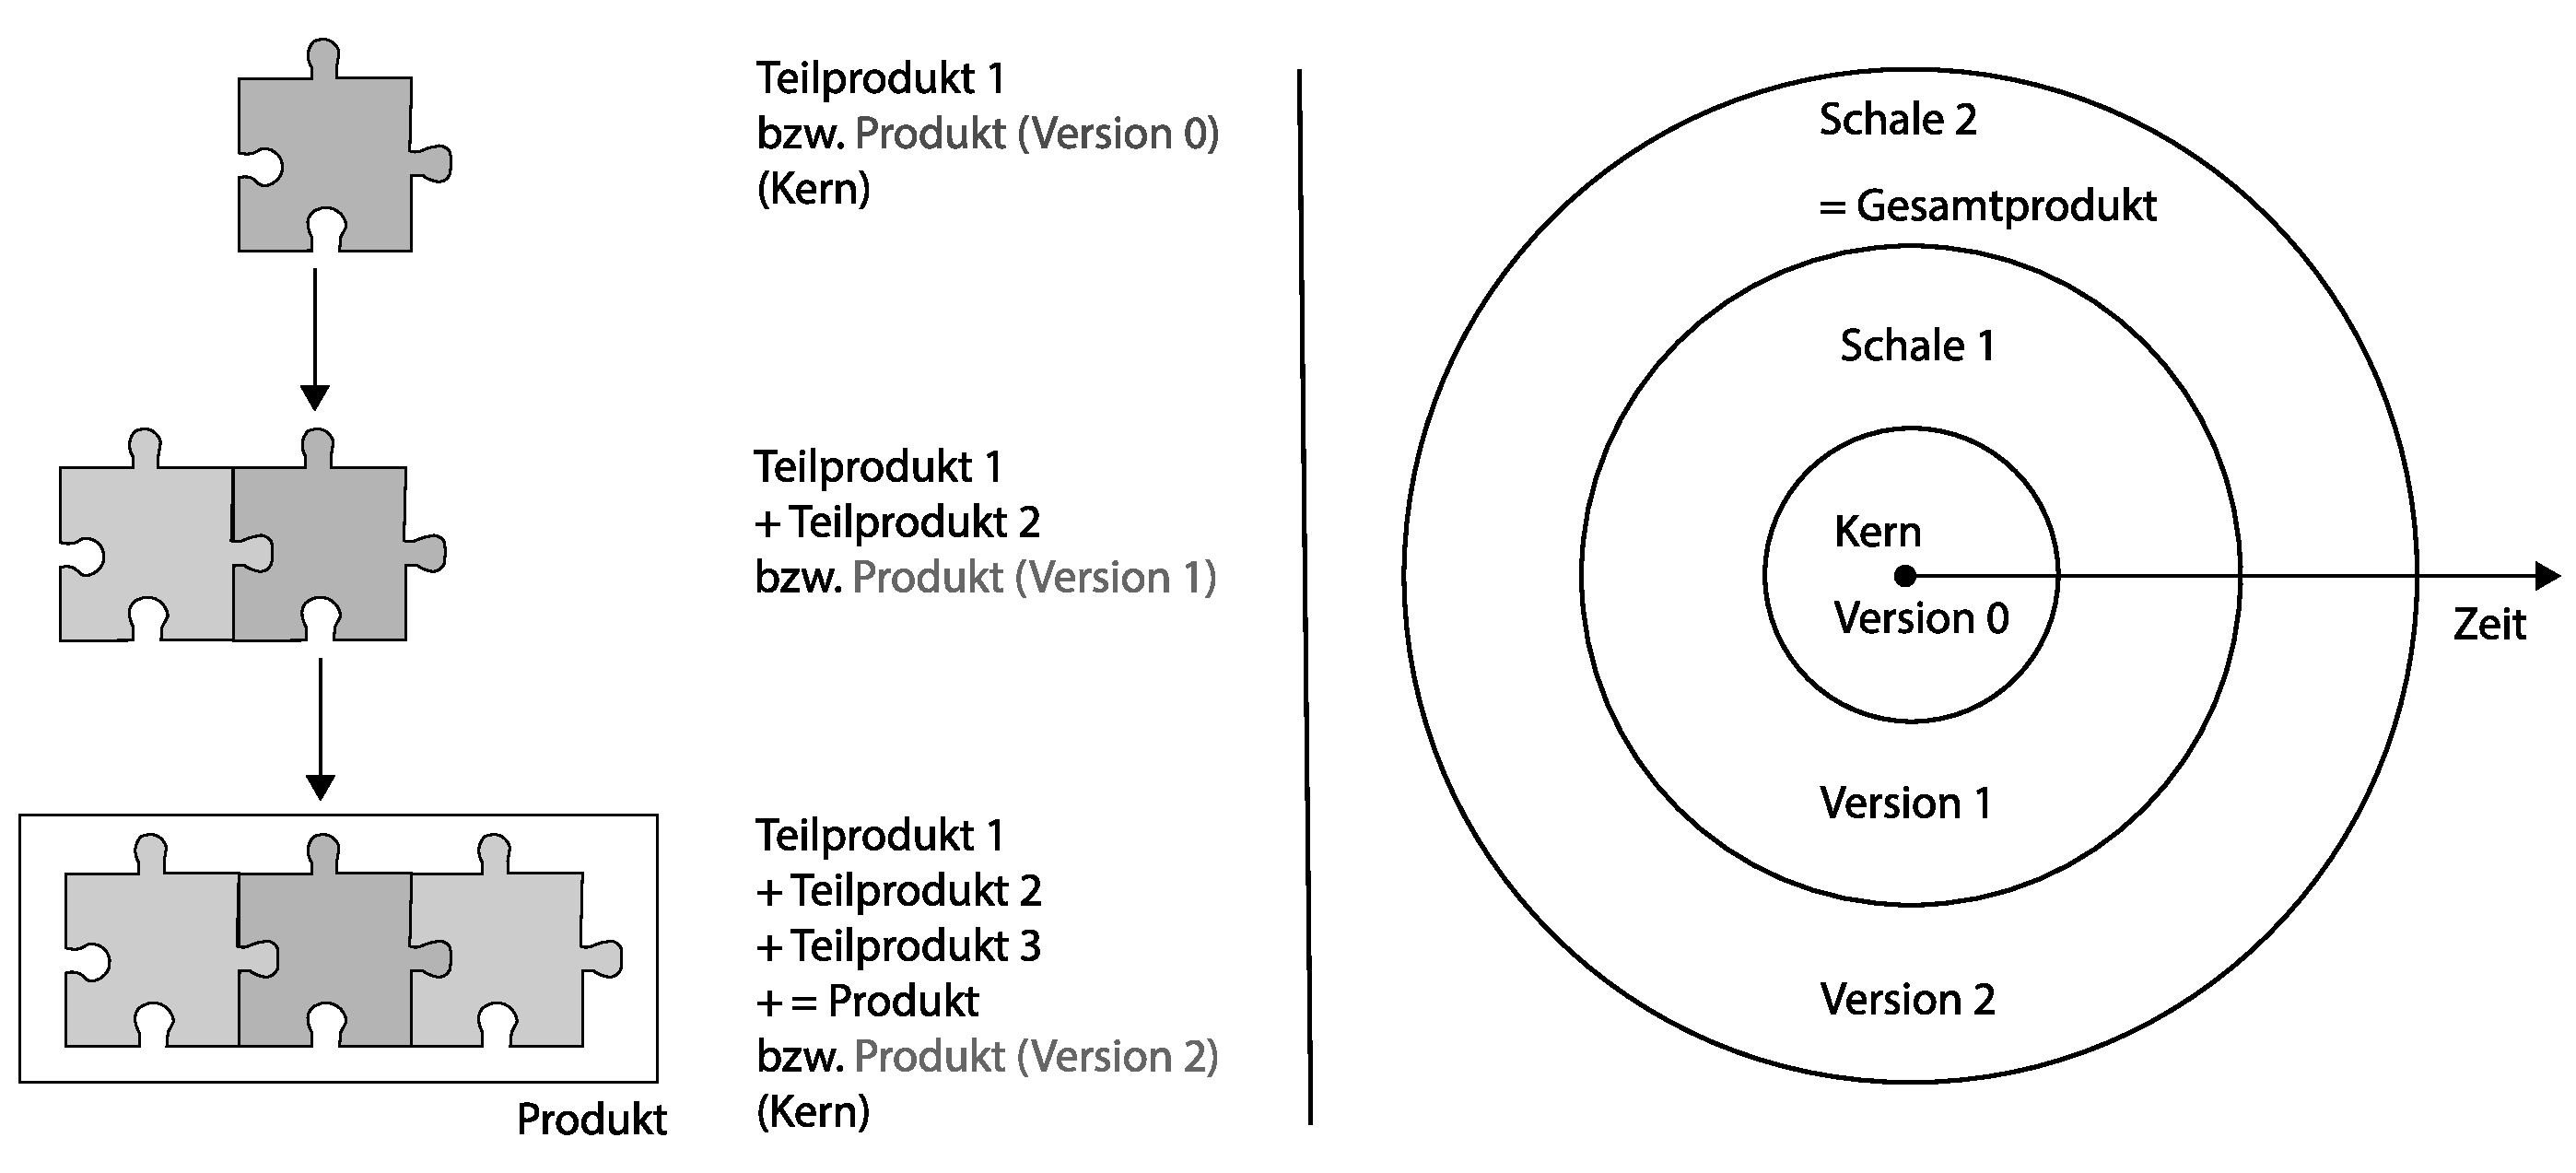
\includegraphics[width=1.2\textwidth]{Bilder/Kapitel-2/PuzzleZwiebel.pdf}
		\caption[Puzzleförmige und zwiebelschalenförmige inkrementelle Entwicklung]{Puzzleförmige (links) und zwiebelschalenförmige (rechts) inkrementelle Entwicklung, nach \cite[527]{bal08}}
		\label{fig:inkrementelle_entwicklung}
	\end{addmargin*}
	\end{addmargin*}
\end{figure}

Welche der beiden Arten 
\marginline{Entwicklungs\-prozess}
für ein konkretes Softwareentwicklungsprojekt eingesetzt werden sollte, hängt in erster Linie davon ab, in welcher Weise sich die Anforderungen an das Gesamtprodukt auf die geplanten Teilprodukte aufteilen lassen. Wenn sich die gewünschten Funktionalitäten annähernd eindeutig bestimmten Teilprodukten (\zb eine Passagierverwaltung und eine Flugzeugverwaltung für ein Flugreservierungssystem) zuordnen lassen, wird eher die puzzleartige Variante der inkrementellen Auslieferung zum Einsatz kommen. Bei der Planung der Inkremente müssen die zukünftigen Schnittstellen zwischen den Teilprodukten (in der Abbildung die Aus- und Einbuchtungen der Puzzleteile) dann so definiert werden, dass es im Ideal\-fall nicht nötig ist ein bestehendes Inkrement zu verändern, sobald ein weiteres Inkrement ergänzt wird.  Wenn dagegen geforderte Funktionalitäten unterschiedlicher Teilprodukte dieselbe Basis benötigen, ist es sinnvoll oder sogar zwingend notwendig, zunächst ein erstes Teilprodukt als Kern des Gesamtsystems zu entwickeln. Jedes weitere Inkrement baut dann so auf der vorherigen Pro\-dukt\-ver\-sion auf, dass es auf Basis der vorherigen Inkremente die Funktionalitäten des Produkts erweitert. Kombinationen beider Varianten der inkrementellen Auslieferung sind auch möglich, zum Beispiel falls alle Teilprodukte nur einen gemeinsamen Kern benötigen, ansonsten aber nicht aufeinander aufbauen müssen.

Die Entwicklung der Teilprodukte – auch bei puzzleförmiger Aufteilung – findet in der Regel nicht parallel, sondern zumindest versetzt statt (\zb Teilprodukt 1 schon im Einsatz, Teilprodukt 2 in der Entwicklung, Teilprodukt 3 in der Planung etc.). Dies dient auch dem Ziel, (positive und negative) Erfahrungen der Nutzer mit einer Produktversion bei der Erstellung der nächsten (erweiterten) Produktversion nach Möglichkeit berücksichtigen zu können. Eine grundlegende Überarbeitung schon ausgelieferter Teilprodukte sehen inkrementelle Modelle nicht vor; schon existierende Funktionalität wird – außerhalb von Fehlerbehebung und Schnittstellenanpassung – nicht verändert.

\sttpHervorhebung{\textbf{Inkrementelle Modelle}}
\marginline{Umgang mit Anforderungen}
\sttpHervorhebung{\textbf{erfordern eine klare Aufteilung der Anforderungen auf die Teilprodukte.}}
Zu Projektbeginn müssen die zentralen Anforderungen an das Gesamtprodukt soweit spezifiziert werden, dass eine Aufteilung in Teilprodukte und die Definition der Schnittstellen zwischen den Teilprodukten möglich sind. Detailliertere Entwurfs- und Implementierungstätigkeiten sind dann zunächst nur für das als erstes auszuliefernde Teilprodukt erforderlich. Der Einsatz inkrementeller Modelle erfordert die gewünschten Funktionalitäten des zukünftigen Softwareprodukts klar voneinander abzugrenzen, um sie den geplanten Inkrementen zuordnen und die Schnittstellen zwischen den Inkrementen definieren zu können. Dafür müssen insbesondere die Abhängigkeiten zwischen einzelnen Anforderungen noch detaillierter analysiert werden als bei Einsatz eines sequentiellen Vorgehensmodells. 

Abhängig vom konkreten inkrementellen Modell muss die (zukünftige) Anzahl der Inkremente zu Beginn des Softwareentwicklungsprojekts festgelegt werden, oder es können im Laufe des Projekts weitere (zukünftige) Inkremente definiert werden. Diese Frage ist eng verknüpft mit der Möglichkeit bzw. Unmöglichkeit im Laufe der Entwicklung neue Anforderungen zu berücksichtigen. Inkrementelle Modelle mit sequentiellem Charakter sehen vor, die vollständigen Anforderungen für alle zukünftigen Teilprodukte schon zu Projektbeginn zu erfassen, noch bevor mit Entwicklungstätigkeiten für das erste Teilprodukt begonnen wird. Andere inkrementelle Modelle sind diesbezüglich flexibler, haben dafür aber ein höheres Risiko, dass die zu Projektbeginn vorgesehene Architektur des Systems für die noch zu berücksichtigenden Anforderungen weniger gut oder im schlimmsten Fall gar nicht geeignet ist. In jedem Fall können neue oder veränderte Anforderungen an das Gesamtprodukt nur dann Berücksichtigung finden, wenn sie sich gut in noch zu entwickelnde Teil\-produkte integrieren lassen bzw. die Möglichkeit besteht zusätzliche Teilprodukte zu definieren. 

\sttpHervorhebung{\textbf{Inkrementelle Modelle}}
\marginline{Einbezug Kunde}
\sttpHervorhebung{\textbf{beziehen den Kunden stärker ein als sequen\-tiel\-le Modelle.}}
Inkrementelle Softwareentwicklung hat im Vergleich zu einem rein sequentiellen Vorgehen den Vorteil, dass der Kunde deutlich schneller eine erste einsetzbare Produktversion bekommt. Diese erste Produktversion kann zum Beispiel den Kern des zukünftigen Gesamtprodukts bilden, oder die für den Kunden wichtigsten Funktionalitäten beinhalten, oder die bezüglich des Entwicklungsaufwands am schwierigsten zu planenden Anforderungen umsetzen. In jedem Fall werden bei Einsatz von inkrementellen Modellen Missverständnisse oder Unklarheiten zwischen dem Entwicklungsteam und dem Kunden (\zb bezüglich der Anforderungen) früher sichtbar als bei sequentiellen Modellen. Das Risiko des kompletten Scheiterns des Softwareentwicklungsprojekts kann so verringert werden. Zudem können zwischen Auftraggeber und Auftragnehmer anstelle eines einzigen Vertrags über die Entwicklung des Gesamtprodukts auch (zeitversetzt abgeschlossene) Verträge für einzelne Teilprodukte vereinbart werden.

Inwieweit der Kunde in den konkreten Entwicklungsprozess der Teilprodukte einbezogen wird, hängt vom konkret eingesetzten inkrementellen Modell ab. Folgt es eher sequentiellen Ansätzen, wird der Kunde nur für Prozesse der Anforderungsermittlung und für die Abnahme der einzelnen Teilprodukte einbezogen. Inkrementelle Modelle, die auch Methoden aus dem agilen Umfeld einsetzen, beinhalten dagegen in der Regel institutionalisiertes und durchgehendes Feedback des Kunden über den gesamten Zeitraum der Entwicklung.

Wie in Abschnitt~\ref{sec:Kap-2.2.1} erwähnt, 
\marginline{Artefakte} 
sind \textbf{sequentielle} Modelle in der Regel dokumentenorientiert. Bezüglich der inkrementellen Modelle finden sich in der Literatur in dieser Hinsicht unterschiedliche Darstellungen. Dies ist wieder der großen Spannweite inkrementeller Modelle geschuldet. Inkrementelle Modelle, die sequentielle \mbox{Methoden} einsetzen, werden eher dokumentenorientiert sein; inkrementelle Modelle mit iterativen oder agilen Methoden eher code- oder testorientiert.


\minisec{Iterative Modelle}

Im Unterschied zu (klassisch) inkrementellen Modellen ist es essentieller Bestandteil von \textit{iterativen Modellen}, dass auch lauffähige (und auch schon ausgelieferte) Produktversionen verändert werden; zum Beispiel weil sich Anforderungen geändert haben bzw. zuvor noch nicht detailliert erfasst waren, neue Anforderungen hinzugekommen sind, Entwurfsentscheidungen revidiert werden, auf neuere Technologien gesetzt werden soll etc. 

Wie bei den inkrementellen Modellen ist die Spannweite an Modellen, die man als iterative Modelle bezeichnen könnte, groß. Am einen Ende stehen sequentielle oder inkrementelle Modelle, wenn sie in größerem Umfang auch iterative Methoden einsetzen. Am anderen Ende stehen die agilen Modelle, die gleichzeitig iterative Modelle sind.

Ziel von iterativen Modellen ist die Verbesserung des Softwareprodukts mit jeder Überarbeitung. Verbessern kann heißen, dass neue Funktionalität hinzugefügt wird, aber auch, dass Aspekte wie die Bedienbarkeit der Software, die Wiederverwendbarkeit einzelner Komponenten, die Schnittstellen zu anderen Systemen oder auch die interne Datenstruktur überarbeitet werden. Dabei ist es möglich, Arbeiten aus vorherigen Iterationen wieder zu verwerfen. Die Dauer einer Iteration hängt stark vom konkreten Softwareentwicklungsprojekt ab. In der Regel liegt sie zwischen einigen Wochen und wenigen Monaten und ist damit deutlich geringer als die Entwicklungszeit eines Inkrements – sprich eines kompletten Teilprodukts – in klassisch inkrementellen Modellen.

\sttpHervorhebung{\textbf{Iterative Modelle}} 
\marginline{Entwicklungs\-prozess}
\sttpHervorhebung{\textbf{durchlaufen die Kernprozesse des Softwareengineering in Zyklen.}} 
In iterativen Vorgehensmodellen wird zunächst anhand einiger Basis\-anforderungen eine erste Kernversion, teilweise auch Nullversion genannt, entwickelt. Kennzeichnend (und namensgebend) für die iterativen Modelle ist, dass die Prozesse des Softwareengineering ausgehend von dieser Kernversion im weiteren Verlauf der Produktentwicklung wiederholt durchlaufen werden und mit jedem Zyklus (jeder Iteration) eine neue, erweiterte oder angepasste Produktversion entsteht, die die vorherige ablöst. Das erinnert auf den ersten Blick an die oben dargestellte zwiebelschalenförmige inkrementelle Entwicklung. Im Gegensatz zu dieser ist die (unter Umständen auch weitreichende) Überarbeitung der aktuellen Version aber ein zentrales Kennzeichen iterativer Modelle. Im Unterschied zu sequentiellen Modellen sind die einzelnen Softwareengineering-Prozesse in iterativen Modellen zudem in der Regel deutlich schwächer voneinander abgegrenzt. So können zum Beispiel Entwurfs- und Implementierungstätigkeiten oder Implementierungs- und Testtätigkeiten eine Einheit bilden und Hand in Hand stattfinden. Und selbst wenn die einzelnen Prozesse innerhalb einer Iteration nacheinander ausgeführt werden, werden sie nicht wie in sequentiellen Modellen durch formale Meilensteine voneinander getrennt. 

\begin{figure}[h!]
	\centering
	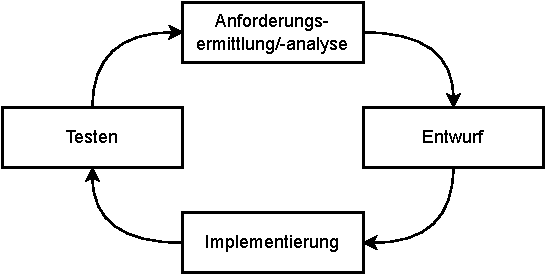
\includegraphics[scale=1.0]{Bilder/Kapitel-2/Abb-2-9.pdf}
	\caption[Iterative Softwareentwicklung]{Iterative Softwareentwicklung. Eine Iteration entspricht einem Zyklus in der Abbildung. Die mögliche zwischenzeitige Auslieferung von lauffähigen Versionen ist hier in der Abbildung nicht berücksichtigt.}
	\label{fig:iterative_softwareentwicklung}
\end{figure}

Durch die Entwicklung des Produkts als Folge von Iterationen kann das Entwicklungsteam von den gesammelten Erfahrungen während einer Iteration profitieren und damit nicht nur das Produkt, sondern auch die Arbeitsprozesse in den folgenden Iterationen optimieren. Im Unterschied zu sequentiellen Modellen, bei \mbox{denen} die verschiedenen Phasen (\zb Entwurf, Implementierung) sehr unter\-schied\-liche Arbeitsprozesse verlangen, sind sich die einzelnen Entwicklungsabschnitte eines iterativen Modells deutlich ähnlicher: die Prozesse des Softwareengineering werden in jeder Iteration erneut durchlaufen – wenn auch in einigen Vorgehensmodellen mit unterschiedlicher Schwerpunktsetzung. Somit können als ungünstig empfundene Arbeitsprozesse einer Iteration direkt in der nächsten Iteration verbessert werden. Ähnliches gilt übrigens auch für die eingesetzten Softwareentwicklungswerkzeuge  (\zb Entwicklungsumgebungen, Modellierungstools, Test-Frameworks). %\sttpgls{CASE_Tools}
Diese können in folgenden Iterationen gewechselt werden, wenn andere Werkzeuge geeigneter erscheinen. In sequentiellen Modellen können positive und negative Erfahrungen mit durchgeführten Arbeitsprozessen oder eingesetzten Werkzeugen dagegen erst im nächsten Softwareentwicklungsprojekt berücksichtigt werden.

\sttpHervorhebung{\textbf{In iterativen Modellen}}
\marginline{Einbezug Kunde}
\sttpHervorhebung{\textbf{wird der Kunde frühzeitig einbezogen.}}
Die Entwicklung in Iterationen erleichtert es, den Kunden in den Entwicklungsprozess einzubinden, zum Beispiel indem nach Abschluss jeder Iteration Rückmeldungen des Kunden eingeholt werden. Dabei besteht die Möglichkeit, anhand der aktuellen Version bzw. des aktuellen Stands Anforderungen für die nächste Version bzw. den nächsten Entwicklungsabschnitt zu verfeinern oder sogar neue Anforderungen zu spezifizieren. Gerade nicht technisch versierten Kunden fällt es sehr viel leichter, auf Grundlage schon funktionierender Software bzw. Prototypen Anforderungen oder Änderungswünsche zu äußern.
%\sttpgls{Prototyp} 

Um  Rückmeldung vom Kunden zu erhalten, kann die aktuelle Produktversion produktiv eingesetzt werden, der Kunde seine Erfahrungen sammeln und für die nächste Version kommunizieren. Rückmeldung kann aber auch heißen, dass die Version nur im Rahmen einer Produktvorstellung vom Kunden kommentiert wird und nicht produktiv eingesetzt wird. Bei letzterer Variante kann es sich dann um lauffähigen Code handeln – die Version somit potentiell produktiv einsetzbar sein – muss es aber nicht (\zb nur animierte Benutzungsschnittstellen). Für produktiv eingesetzte Versionen wird in der Literatur manchmal der Begriff \textit{Release}
\marginline{Release}
verwendet, der auch im Umfeld agiler Modelle verbreitet ist.

\pagebreak %%% für Druck

\sttpHervorhebung{\textbf{Iterative Modelle berücksichtigen Anforderungsänderungen.}} \marginline{Umgang mit Anforderungen}
Iterative Vorgehensmodelle können durch die kürzeren Entwicklungszyklen und die stärkere Einbindung des Kunden besser als inkrementelle Modelle und deutlich besser als sequentielle Modelle mit zusätzlichen oder veränderten Anforderungen während der Projektlaufzeit umgehen. Zudem tragen sie explizit der Tatsache Rechnung, dass es auch bei zu Projektbeginn feststehenden und stabilen Anforderungen aufgrund von Missverständnissen zwischen Kunden und Entwicklungsteam vorkommen kann, dass die Umsetzung nicht den (eigentlichen) Wünschen des Kunden entspricht. 

Iterative  Modelle sind daher gut geeignet, wenn die Funktionalitäten des zukünftigen Produkts zu Beginn der Entwicklung noch nicht komplett feststehen oder auf Änderungen während der Entwicklung reagiert werden soll. Letzteres bezieht sich im Übrigen nicht nur auf Änderungen der Anforderungen, sondern auch auf technologische Änderungen (\zb Verfügbarkeit passenderer Frameworks). Auf der anderen Seite besteht bei iterativen Modellen immer die Gefahr, dass die für die Kernversion gewählte Systemarchitektur sich in späteren Iterationen als zu unflexibel für den Einbau weiterer Funktionalität herausstellt und (aufwändig) überarbeitet werden muss. Diese Gefahr ist umso größer, je weniger klar der Kunde die Funktionalitäten des zukünftigen Softwareprodukts zu Projektbeginn spezifizieren kann. Wenn die fachlichen oder technologischen Unsicherheiten des Produkts zu Projektbeginn sehr groß sind, kann es sinnvoll sein iterative Modelle zusätzlich mit Verfahren aus dem Prototyping 
%\sttpkapitelverweis{Pro\-to\-typen\-ent\-wick\-lung}{Kap.~\ref{sec:Kap-7}}
zu verbinden. 

Aus Managementsicht liegt eine Schwierigkeit von iterativen Modellen in der Kontrolle des Projektfortschritts. Wenn zu Beginn des Entwicklungsprojekts nicht komplett feststeht, über welche Funktionalitäten das zu entwickelnde Produkt bei Fertigstellung verfügen wird, ist es während der Projektlaufzeit schwierig bis unmöglich zu beurteilen, ob der Entwicklungsfortschritt zu einem bestimmten Zeitpunkt im Zeitrahmen liegt oder nicht. Ebenfalls aufgrund der nicht vollständigen Spezifizierung der Anforderungen zu Projektbeginn ist auch die Vertragsgestaltung kompliziert, wenn ein Softwareprodukt nicht für das eigene Unternehmen, sondern für einen Auftraggeber entwickelt werden soll. Dieses Problem wurde in den 2000er Jahren mit dem stärkeren Einsatz agiler Vorgehensmodelle, bei denen die iterative Entwicklung essentieller Bestandteil ist, weithin sichtbar. Lösungsmöglichkeiten sind vorgeschaltete Prototyping-Projekte und neue Arten von Vertragsmodellen.

\sttpHervorhebung{\textbf{Iterative Modelle sind code- oder testorientiert.}} \marginline{Artefakte}
Codeorientiert bedeutet, dass am Abschluss jeder Iteration Programmcode steht. Iterative Modelle können (darüber hinaus) auch testorientiert sein, wenn Iterationen eine Menge zuvor spezifizierter Testfälle zugrunde liegen, die die jeweilige Produktversion der Software erfüllen soll. Basis für solche Testfälle können zum Beispiel typische Arbeitsabläufe sein, die die zukünftige Software unterstützen soll. 
%\sttpkapitelverweis{Use Cases}{Kap.~\ref{sec:Kap-6.2.1.1}}
%\sttpkapitelverweis{User Stories}{Kap.~\ref{sec:Kap-6.2.1.2}}

Anders als bei sequentiellen Modellen entstehen bei iterativen Modellen aufgrund der Verschmelzung der Softwareengineering-Prozesse und der starken Codeorientierung nicht automatisch während des Entwicklungsprozesses (Meilenstein)-Dokumente, wie eine strukturierte Auflistung der Anforderungen, eine Übersicht über alle Komponenten der Software, eine detaillierte Beschreibung einzelner Funktionen oder auch eine Historie getroffener Entwurfsentscheidungen etc. Eine Schwierigkeit iterativer Modelle besteht daher darin, wie das zukünftige Produkt und getroffene Entscheidungen dokumentiert werden. Eine entsprechende Dokumentation müsste parallel zur Implementierung innerhalb einer Iteration erstellt und bei Änderungen in späteren Iterationen immer wieder angepasst werden. Es ist stark abhängig vom konkreten Softwareentwicklungsprojekt, wie weitreichend eine Dokumentation des Systems und der getroffenen Entscheidungen in iterativen Modellen vorgenommen wird. Die minimale Variante ist der weitgehende Verzicht einer externen Dokumentation, indem der Programmcode möglichst „selbsterklärend“ gestaltet wird und nur um absolut notwendige Kommentare sowie um Funktionalitätsbeschreibungen von Schnitt\-stellen ergänzt wird. Weitergehendere Varianten wären die zusätzliche externe (und in späteren Iterationen jeweils anzupassende) Dokumentation der Anforderungen zum Beispiel anhand von User Stories oder die Dokumentation der Systemstruktur zum Beispiel anhand von Komponenten- und Klassendiagrammen. %\sttpkapitelverweis{Komponenten\-diagramme}{Kap.~\ref{sec:Kap-6.1.2}}
%\sttpkapitelverweis{Klassendiagramme}{Kap.~\ref{sec:Kap-3.2.4}} 
Weitreichende externe Dokumentationen dokumentieren darüber hinaus auch getroffene Entscheidungen und ihre Gründe – sei es klassisch in Form von Dokumenten oder agiler über Wikis oder Ticketsysteme –, um validere Folgeabschätzungen zu ermöglichen, falls getroffene Entscheidungen im späteren Projektverlauf revidiert werden müssen.

Das erste Vorgehensmodell, das umfangreichere Iterationen vorsah, war Ende der 1980er Jahre das Spiralmodell von Barry W. Boehm (\cite{boe86} und \cite{boe88}). Aus heutiger Sicht liegt die Bedeutung des Spiralmodells vor allem darin, dass es schon in den 1980er Jahren – und damit zur Hochzeit der phasenorientierten Modelle – ein iteratives Vorgehen und den Einsatz von Prototypen für die Entwicklung eines Softwareprodukts propagierte. Deutlich bekannter geworden ist aber der  im Zuge der objektorientierten Programmierung in den 1990er Jahren groß gewordene (Rational) Unified Process.

\sttpAutorenkasten{Barry W. Boehm}{1935}{2022}{
	\vspace{2mm} %%% für Druck
	US-amerikanischer Software\-ingenieur. Neben seiner Arbeit an Vorgehensmodellen ist er vor allem für das COCOMO-Modell bekannt. COCOMO (Constructive Cost Model) ist ein algorithmisches Modell, mit dem Kosten und Aufwand von geplanten Softwareprojekten geschätzt werden können.
	\vspace{2mm} %%% für Druck
}{Bilder/Autoren/boehm.jpg}{2006}{Improve it, \href{https://creativecommons.org/licenses/by-sa/2.0}{CC BY-SA 2.0}, via \href{https://commons.wikimedia.org/wiki/File:O_lend\%C3\%A1rio_Barry_Boehm.jpg}{Wikimedia Commons}}


\clearpage %%% für Druck

\subsubsection{Unified Process und Rational Unified Process}
\label{sec:Kap-2.2.2.1}

\vspace{\baselineskip} %%% für Druck

\sttpLeserfuehrung{Bilder/Kapitel-2/Leserfuehrung/vorgehensmodelle_iterativ_inkrementell_illustration.pdf}{Bilder/Kapitel-2/Leserfuehrung/vorgehensmodelle_rational_unified_process.pdf}

Ein  Kritikpunkt am Wasserfallmodell (und anderen Modellen der 1980er Jahre) war die starke Fokussierung auf rein softwaretechnische Aspekte und der damit niedrige Stellenwert der fachlichen Belange des Anwendungsbereichs des zu erstellenden Softwareprodukts. Das betraf den Einbezug zukünftiger Nutzer des Softwareprodukts ebenso wie den Umgang mit sich ändernden oder neuen Anforderungen aus der Domäne. Der Ende der 1990er Jahre im Zusammenhang mit der Unified Modelling Language (UML) entstandene und speziell auf objektorientierte Softwareentwicklung ausgerichtete Unified Software Development Process (kurz: Unified Process) \cite{jac99} legte den Fokus erstmals auf die Domäne und die Erfassung der dortigen Geschäftsprozesse. Der Unified Process selber ist ein sehr allgemein gehaltenes Vorgehensmodell, das zwar die Struktur des Vorgehens vorgibt, in den Details aber sehr unterschiedlich ausgestaltet werden kann. Von den verschiedenen Ausgestaltungen des Unified Process ist der Rational Unified Process die bekannteste Version.

Der von der Firma Rational Software (seit 2003 zu IBM gehörig) entwickelte Rational Unified Process (RUP) ist eine stark ausdifferenzierte und werkzeuggestützte Version des Unified Process. Er ist nicht nur ein Vorgehensmodell, sondern auch eine eigenständige Software-Suite, die verschiedene Entwicklungswerkzeuge anbietet, die auf Grundlage des Vorgehensmodells den Entwicklungsprozess eines konkreten Softwareentwicklungsprojekts unterstützen. 

\minisec{Struktur des Softwareentwicklungsprozesses}

Abbildung~\ref{fig:struktur_des_RUP} zeigt die Struktur des RUP. Der RUP unterscheidet die vier in der Abbildung in den Spalten dargestellten Phasen Konzeption (engl. inception), Ausarbeitung (elaboration), Konstruktion (construction) und Übergang in den Betrieb (transition), die nacheinander stattfinden. Jede Phase ist wiederum in Teilphasen (explizit \textit{Iterationen} \marginline{Iterationen}
genannt) aufgeteilt. Die Anzahl der Iterationen pro Phase ist nicht vorgegeben, sondern abhängig vom konkreten Softwareentwicklungsprojekt; die in der Abbildung dargestellte Anzahl der Iterationen daher nur beispielhaft. Im Gegensatz zu den Phasen eines Wasserfallmodells handelt es sich bei den RUP-Phasen nicht um die Prozesse des Softwareengineering, sondern um eine Aufteilung der Entwicklung in vier große Abschnitte, die jeweils mit Meilensteinen abgeschlossen werden und Auskunft über den Stand der Produktenwicklung geben. Die Prozesse des Softwareengineering bildet der RUP in sogenannten Disziplinen (engl. disciplines; in der Abbildung in den Zeilen dargestellt) ab. Hier werden die Prozesse Geschäftsprozessmodellierung (Business Modeling), Anforderungsermittlung (Requirements), Analyse und Entwurf (Analysis and Design), Implementierung (Implementation), Test (Test) und Auslieferung/Inbetriebnahme (Deployment) als sogenannte \textit{Kerndisziplinen}  sowie die \textit{unterstützenden Disziplinen} 
\marginline{Kerndisziplinen, unterstützende Disziplinen}
Konfigurations- und Änderungs\-manage\-ment (Configuration and Change Management), Projekt\-manage\-ment (Project Manage\-ment) und Entwicklungsinfrastruktur (Environment) unterschieden.

\vspace{-2mm} %%% für Druck

\begin{figure}[h!]
	\centering
	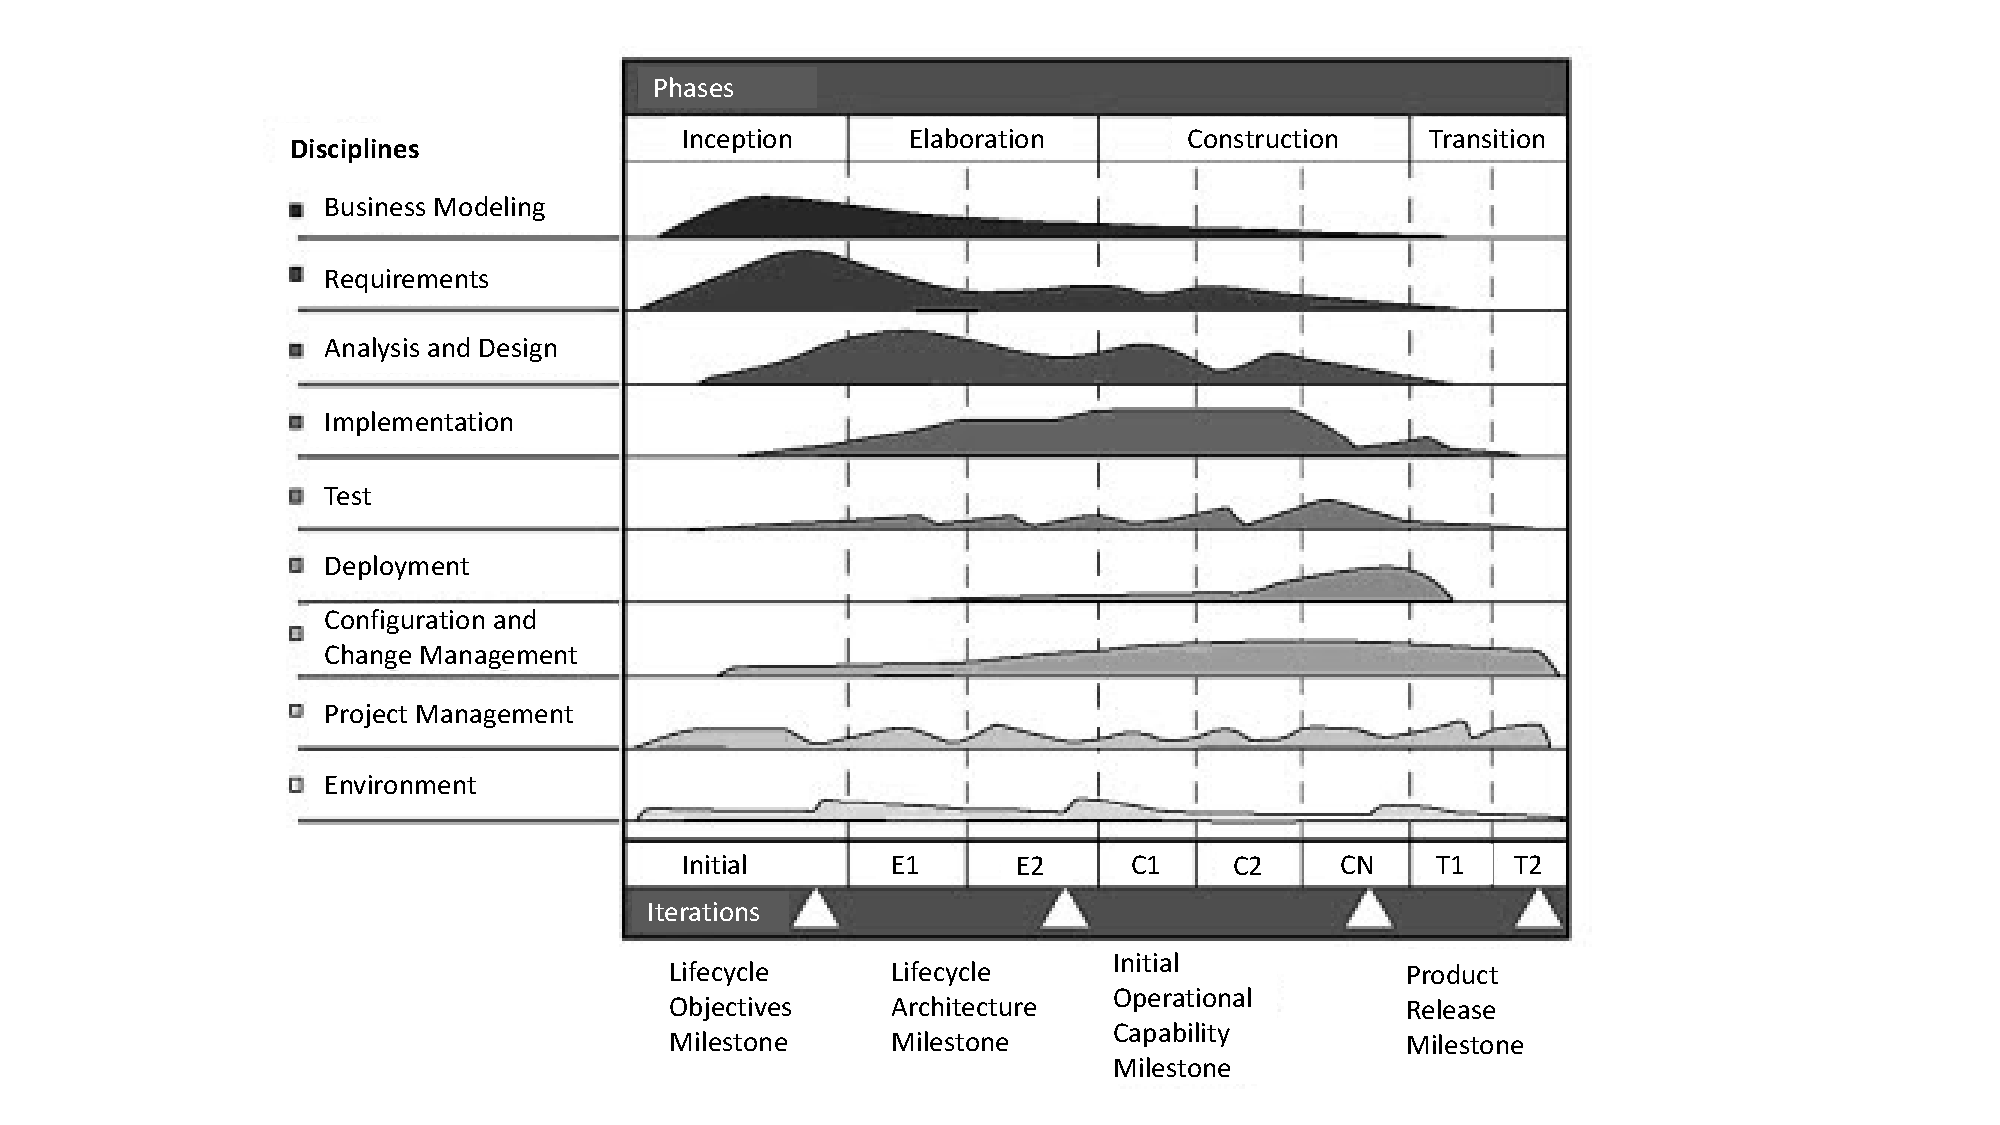
\includegraphics[width=\textwidth]{Bilder/Kapitel-2/StrukturRUP.pdf}
	\caption[Struktur des Rational Unified Process]{Struktur des Rational Unified Process, nach \cite[8]{shu08}}
	\label{fig:struktur_des_RUP}
\end{figure}

\vspace{-2mm} %%% für Druck

Der RUP adressiert mit den drei letztgenannten unterstützenden Disziplinen explizit auch diejenigen Aufgaben, die in einem Softwareentwicklungsprojekt außerhalb der reinen softwaretechnischen Prozesse durchzuführen sind. Innerhalb der Disziplin Projektmanagement nehmen dabei die Durchführung von Machbarkeitsstudien und Wirtschaftlichkeitsprüfungen, aber auch die Verwaltung von Risiko\-management\-plänen einen deutlich höheren Stellenwert ein als bei vielen anderen Vorgehensmodellen. Die Disziplin Entwicklungsinfrastruktur beinhaltet alle Aspekte, die die Bereitstellung von Hardware und Software für das Entwicklungsprojekt betreffen. Die Disziplin Konfigurations- und Änderungsmanagement beinhaltet Aufgaben, die sicherstellen, dass die im Projekt erstellten Dokumente verwaltet und ihre Konsistenz gewährleistet wird. Dazu gehört auch die Pflege einer Versionshistorie. 

In jeder Iteration sollen alle Disziplinen durchlaufen werden, allerdings mit verschiedener Schwerpunktsetzung. Dies verdeutlicht die Abbildung durch die unterschiedlich (und nur idealtypisch) verlaufenden Kurven in den Zeilen der Disziplinen. Je mehr Fläche unterhalb einer Kurve eingezeichnet ist, desto mehr Aufgaben aus dem Bereich der entsprechenden Disziplin werden während der jeweiligen Iteration durchgeführt. So haben zum Beispiel die Disziplinen Geschäftsprozessmodellierung und Anforderungsermittlung ihren Schwerpunkt in der Phase Konzeption, während die Implementierung hauptsächlich zum Ende der Ausarbeitung sowie während der Konstruktionsphase stattfindet. Im Vergleich zu Wasserfallmodellen ist somit nicht jeder Softwareengineering-Prozess fest zugeordnet, sondern wird in jeder Phase (wiederholt) durchlaufen. Insbesondere auch die bei Wasserfallmodellen kritisierte Ver\-ortung von Testaktivitäten löst der RUP dadurch besser. Eine gewisse Ähnlichkeit mit sequentiellen Vorgehensmodellen besteht allerdings doch, da die Schwerpunktsetzung der Kerndisziplinen in den Phasen der aus den sequentiellen Modellen bekannten Reihenfolge Anforderungsermittlung-""Entwurf-""Implementierung-""Testen folgt, auch wenn beim RUP grundsätzlich alle Disziplinen in allen Phasen aktiv sind. Auch Meilensteine am Ende von Phasen sind Charakteristika eines sequen\-tiel\-len Vorgehens, wobei die konkrete Ausgestaltung der Meilensteine im RUP (ausführbarer Architekturprototyp am Ende der zweiten Phase und Beta-Version des Softwareprodukts am Ende der dritten Phase) dann doch eher untypisch sind für sequentielles Vorgehen. 

\vspace{2mm} %%% für Druck

\minisec{Umgang mit Anforderungen}

Im  Vergleich zu vielen anderen Vorgehensmodellen werden im RUP zu Beginn eines Entwicklungsprojekts intensiv die durch das zu entwickelnde Softwareprodukt durchzuführenden oder zu unterstützenden Geschäftsprozesse der Domäne betrachtet. Innerhalb der Disziplin Geschäftsprozessmodellierung werden dafür mithilfe von Anwendungsfall\-mo\-dellen der UML %\sttpkapitelverweis{An\-wen\-dungs\-fall\-mo\-del\-le}{Kap.~\ref{sec:Kap-6.2.1}}
die relevanten Prozesse der Domäne dokumentiert oder auch spezifiziert, falls es sich um zu verändernde oder neu zu schaffende Geschäftsprozesse handelt. Das erfordert eine starke Einbindung der zukünftigen Nutzer des Softwareprodukts, da in der Regel nur diese die vertiefte Kenntnis über die Domäne besitzen. Die erstellten Anwendungsfallmodelle sind eine zentrale Grundlage für die Ermittlung bzw. zum Verständnis der funktionalen Anforderungen 
%\sttpkapitelverweis{funktionale Anforderungen}{Kap.~\ref{sec:Kap-6.1.3.2}}
des zu entwickelnden Softwareprodukts.

Im Rahmen der Disziplin Konfigurations- und Änderungsmanagement werden die Verfahrensweisen für den Umgang mit neuen oder sich ändernden Anforderungen während der Projektlaufzeit festgelegt. Der RUP ist deutlich flexibler bezüglich neuer Anforderungen als sequentielle Modelle, da über das definierte Änderungs\-management auch in späteren Projektphasen grundsätzlich noch Anforderungsänderungen möglich sind. Weitgehende Ergänzungen oder Änderungen der Anforderungen werden aber in der Regel erst in späteren Inkrementen bzw. Entwicklungszyklen berücksichtigt.

\vspace{2mm} %%% für Druck

\minisec{Artefakte des Entwicklungsprozesses}

Der RUP legt sehr detailliert fest, welche Aufgaben im Rahmen der Disziplinen auszuführen sind. Dafür definiert er zahlreiche verschiedene Rollen und Artefakte und spezifiziert detaillierte Prozessbeschreibungen, die Auskunft darüber geben, welche Aktivitäten durch welche Rollen zu welchen Zeitpunkten im Rahmen der Arbeitsabläufe welche Ergebnisse produzieren. Damit ist der RUP ein sehr detaillierendes Vorgehensmodell, das vor Projektstart an die spezifischen Bedürfnisse des konkreten Softwareentwicklungsprojekts angepasst werden muss (Tailoring, von engl. to tailor sth. = etwas maßschneidern). Diese Anpassung wird durch die Werkzeuge der RUP-Software unterstützt.

Den RUP kann man aufgrund des hohen Stellenwerts der geschäftlichen Anwendungsfälle als anwendungsfallorientiert bezeichnen, auch wenn ähnlich wie bei sequentiellen Modellen viele Artefakte des Entwicklungsprozesses Dokumente sind und somit die Bezeichnung dokumentenorientiert auch nicht falsch wäre.

\vspace{2mm} %%% für Druck

\minisec{Einordnung des RUP}

\vspace{1mm} %%% für Druck

Trotz der durchaus vorhandenen sequentiellen Charakteristika kann man den RUP in die Kategorie iterativ-inkrementelles Vorgehensmodell einordnen: Der wiederholte Durchlauf der Prozesse des Softwareengineering entspricht einem iterativen Vorgehen, auch wenn sich die Schwerpunktsetzung der einzelnen Iterationen unterscheidet. Die Bezeichnung iterativ bezieht sich aber auch darauf, dass komplette Entwicklungszyklen, also die Gesamtfolge der Phasen Konzeption-Ausarbeitung-Konstruktion-Übergang in den Betrieb wiederholt werden. Auf die Auslieferung der ersten Produktversion an den Kunden am Ende der Übergangs-Phase kann eine zweite Konzeptionsphase folgen und damit ein zweiter Entwicklungszyklus für die nächste Produktversion beginnen, die die erste Produktversion ersetzt. Der erste Entwicklungszyklus wird im RUP als \textit{Initialzyklus}, 
\marginline{Initialzyklus, Evolutions\-zyklen} 
die weiteren als \textit{Evolutionszyklen} bezeichnet. Diese Form von Iteration ist der Vorstellung von Iteration, wie sie im Rahmen der agilen Modelle verwendet wird, schon sehr nah. Bei der Wiederholung ganzer Entwicklungszyklen kann es sich statt um iterative aber auch um (klassisch) inkrementelle Entwicklung handeln, sofern die Produktversionen der Entwicklungszyklen eigenständige Teilprodukte bilden und durch spätere Inkremente ergänzt, aber nicht abgelöst werden. Im Falle von inkrementeller Entwicklung ist zudem die parallele Durchführung mehrerer Entwicklungszyklen möglich.

Der RUP definiert neben konkreten Arbeitspaketen grundlegende Prinzipien für die geschäftsprozessorientierte Softwareentwicklung, die aus in der Praxis bewährten Vorgehensweisen und Erfahrungswerten (\textit{Best Practices}) 
\marginline{Best Practices}
hervorgegangen sind. Solche prozessübergreifenden Grundsätze sind häufig auch essentieller Bestandteil agiler Vorgehensmodelle. Neben der Betonung der Wichtigkeit eines kontrollierten Anforderungs- und Änderungsmanagements gehört zu den Grundsätzen des RUP die schon erwähnte iterative anstelle der sequentiellen Entwicklung. Ein weiterer Grundsatz lautet, eine komponentenbasierte Architektur zu entwerfen, um so neben dem projektspezifischen Programmcode auch vorhandene Softwarekomponenten in das zu entwickelnde Softwareprodukt einzubinden. Einen hohen Stellenwert bekommen zudem die grafischen UML-Modelle zugeschrieben, und zwar nicht nur für Zwecke innerhalb des Entwicklungsteams, sondern vor allem auch zur Kommunikation mit Auftraggebern und Nutzern. Die starke Einbeziehung von Nutzern und die komponentenbasierte Entwicklung sind ebenfalls Aspekte, die man auch in agilen Vorgehensmodellen findet.

Seiner Entstehungszeit – zwischen vorherrschenden sequentiellen Modellen und aufkommenden agilen Strömungen – ist es vermutlich geschuldet, dass der RUP neben den ihm eigenen iterativen und inkrementellen Elementen einerseits Charakteristika sequentieller Vorgehensmodelle, andererseits aber auch solche späterer agiler Modelle aufweist. Trotz der agilen Elemente bleibt der RUP aber ein eher 
\marginline{schwer\-gewichtiges Modell}
schwergewichtiges Modell, das während des Softwareentwicklungsprozesses die Erstellung und Pflege zahlreicher Dokumente vorsieht, die später nicht direkter Bestandteil des Softwareprodukts werden. Dies ist die Stelle, an der sich der RUP am deutlichsten von agilen Vorgehensmodellen unterscheidet.
\subsection{Agile Modelle}
\label{sec:Kap-2.2.3}

\sttpLeserfuehrung{Bilder/Kapitel-2/Leserfuehrung/vorgehensmodelle_agile_illustration.pdf}{Bilder/Kapitel-2/Leserfuehrung/vorgehensmodelle_agile.pdf}

In den 1990er Jahren entstanden als Gegenbewegung zu den als schwergewichtig empfundenen vorherrschenden Softwareentwicklungsprozessen, die sich durch stark vorgegebene Abläufe und dokumentenorientierte Vorgehensweisen auszeichneten, sogenannte \textit{leichtgewichtige Modelle}. \marginline{leichtgewichtige Modelle}
Die Befürworter leichtgewichtiger Prozesse argumentierten, dass im Mittelpunkt von Softwareentwicklungsprojekten die Erstellung funktionierender Software und nicht die Abarbeitung von Regeln und das Produzieren von Dokumenten stehen müsse. Dementsprechend plädierten sie für eine Verschlankung und Flexibilisierung der Softwareentwicklungsprozesse. Basierend auf dieser Grundidee entwickelten sich Mitte bis Ende der 1990er Jahre die ersten leichtgewichtigen Vorgehensmodelle – wobei in diesem Kontext der Begriff 
\marginline{Entwicklungs\-modell}
\textit{Entwicklungsmodell} üblicher ist als Vorgehensmodell.

Die Bezeichnung \textbf{agil} für die leichtgewichtigen Modelle entstand, als sich im Februar 2001 in Utah, USA siebzehn Vertreter verschiedener leichtgewichtiger Modelle zu einem Gedankenaustausch versammelten, um Gemeinsamkeiten zwischen den verschiedenen Ansätzen zu finden. Alistair Cockburn, einer der Teilnehmer des Treffens, schrieb im Rückblick, dass der Begriff \textbf{leichtgewichtig} für viele Teilnehmer „eher eine Abneigung gegen etwas vermittelte als Vertrauen in etwas“ \cite[281]{coc03} und daher mit \textbf{agil} ein neuer Begriff gewählt wurde. Mit dieser Begriffswahl sollte zudem hervorgehoben werden, dass man im Laufe eines Softwareentwicklungsprojekts auf Veränderungen reagieren können muss. 

\sttpseitenrandzitat{„After a while we settled on Agile Software Development. Of course organizations would want to be agile. You can explain that to your CEO or customer far more easily than proclaiming you are extreme.“ \cite[16]{hun11}}{James Grenning, einer der Autoren des Agilen Manifests über die Wahl des Begriffs agil für Entwicklungsmethoden, die man bis dahin mit dem Extreme Programming verband.}

Auf  dem Treffen in Utah wurde als gemeinsame Erklärung das sogenannte 
\marginline{das Agile Manifest}
\textit{Agile Manifest} (Abb.~\ref{fig:das_agile_manifest}) verabschiedet. Es beinhaltet die grundlegende Philosophie der agilen Softwareentwicklung in Form von vier als \textit{Werte} bezeichneten Gegenüber\-stellungen. Wichtig ist, dass in diesem Manifest zwar eindeutige Präferenzen für die Aspekte in den ersten Satzhälften (\zb „Reagieren auf Veränderung“) zum Ausdruck gebracht werden, den Aspekten der zweiten Satzhälften (\zb „Befolgen eines Plans“), die dem Umfeld der schwergewichtigen Prozesse entstammen, aber ebenfalls Bedeutung beigemessen wird. So bedeutet zum Beispiel die Priorisierung funktionierender Software nicht zwingend den Verzicht auf eine (auch umfassendere) Dokumentation. Zusätzlich zu den Werten des Manifests einigten sich die Teilnehmer auf zwölf sogenannte \textit{Prinzipien}\footnote{\href{https://agilemanifesto.org/iso/de/principles.html}{https://agilemanifesto.org/iso/de/principles.html}.}, \marginline{Werte, Prinzipien}
die in Form von Handlungsanweisungen detaillierter als die Werte die Basis agiler Softwareentwicklung erläutern.

\begin{figure}[h!]
    \centering
    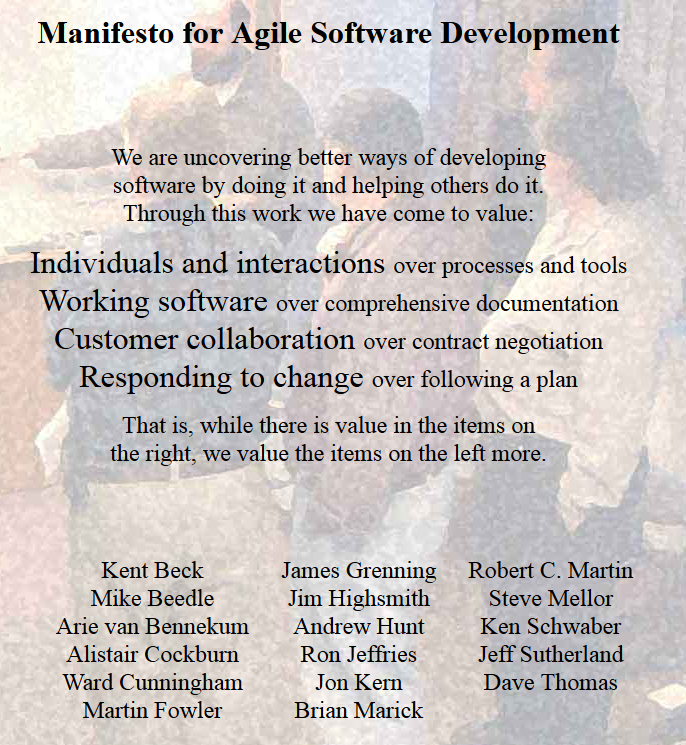
\includegraphics[scale=0.5]{Bilder/Kapitel-2/ScreenshotAgilesManifest.png}
    \caption[Das Agile Manifest]{Das Agile Manifest\\ (Screenshot von \href{https://agilemanifesto.org/iso/en/manifesto.html}{https://agilemanifesto.org/iso/en/manifesto.html})}
    \label{fig:das_agile_manifest}
\end{figure}

Mit der Verabschiedung des Agilen Manifests erfuhren die nun agil genannten Modelle einen – im zustimmenden wie im ablehnenden Sinne – enormen Bedeutungszuwachs. Werte und Prinzipien des Agilen Manifests bilden heute den Rahmen, innerhalb dessen sich – durchaus auch sehr verschiedenartige – Modelle und einzelne Methoden agil nennen. 

Agile Modelle sind immer iterative Modelle – allerdings nicht umgekehrt. Die iterative Entwicklung, in der für jede Produktversion alle Prozesse des Softwareengineering wiederholt durchlaufen werden, ist essentieller Bestandteil agiler Softwareentwicklung. Gleichzeitig sind agile Modelle auch inkrementelle Modelle, da es sich (ab einem gewissen Zeitpunkt im Projekt) zumindest bei Teilen der ausgelieferten Funktionalitäten um fertige Inkremente handelt, die nicht in späteren Versionen überarbeitet werden sollen.

\sttpHervorhebung{\textbf{Agile Modelle}} 
\marginline{Auslieferung}
\sttpHervorhebung{\textbf{liefern kontinuierlich lauffähige Software aus.}} 
Von einer ausgelieferten Produktversion zur nächsten vergehen in der Regel maximal einige Wochen. Aufgrund der kurzen Entwicklungszyklen spielen in agilen Modellen automatisiertes Testen, Verwendung existierender Frameworks und Bibliotheken sowie Einsatz von Entwicklungswerkzeugen eine besonders große Rolle. Erste Ideen und Ansätze, (Teile einer) Software schon während ihres laufenden Entwicklungsprozesses produktiv einzusetzen, hatte es bereits zu den Hochzeiten der Phasenmodelle in den 1980er Jahren gegeben \cite[84-2]{fav14}, aber erst im Kontext der agilen Modelle reiften diese Ideen zu einem grundlegenden Entwicklungsprinzip.

\sttpHervorhebung{\textbf{In agilen Modellen}} 
\marginline{Umgang mit Anforderungen} 
\sttpHervorhebung{\textbf{sind Anforderungsänderungen inhärenter Bestandteil des Softwareentwicklungsprozesses.}} 
Fehlende bzw. stark eingeschränkte Möglichkeiten auf die Änderung von Anforderungen zu reagieren, betrachten die Vertreter agiler Softwareentwicklung als den Hauptgrund für das Scheitern von Softwareentwicklungsprojekten. In agilen Modellen werden zu Beginn eines Softwareentwicklungsprojekts daher in der Regel nur der grobe Produktumfang und die grundlegenden Funktionalitäten (explizit noch in wenig detaillierter Weise) festgelegt. Weitere zu Beginn bekannte Anforderungen werden nur gesammelt (\zb bei Scrum im sogenannten Product Backlog, bei Extreme Programming  in Form von User Stories), ohne Anspruch auf Vollständigkeit der Sammlung und auch ohne Anspruch da\-rauf, dass alle dort gesammelten Anforderungen im Laufe der Produktentwicklung tatsächlich umgesetzt werden. Jegliche Auswahl und detailliertere Spezifikation von umzusetzenden Anforderungen erfolgt erst kurz vor Beginn derjenigen Iteration, in der sie implementiert werden sollen. Dadurch ist es möglich neue Anforderungen, die vom Kunden als prioritär gegenüber schon vorhandenen Anforderungen angesehen werden, vorzuziehen. Die Entscheidung, welche Anforderungen in der jeweiligen Iteration umgesetzt werden, wird in enger Abstimmung zwischen Kunden und Entwicklungsteam getroffen. Diese Flexibilität bezüglich der Anforderungsermittlung und –änderung sehen agile Modelle in der Regel auch für die Softwarearchitektur und eingesetzte Technologien vor (\zb Wechsel der Datenbanktechnologie, Wechsel eingesetzter Frameworks, Änderung der User-Interface-Technologie, Änderung von Server-Client-Zuständigkeiten).

\sttpHervorhebung{\textbf{Agile Modelle}} 
\marginline{Einbezug Kunde}
\sttpHervorhebung{\textbf{binden den Kunden intensiv ein.}} 
Der Kunde wird mindestens immer dann benötigt, wenn die zu realisierenden Anforderungen für die nächste Iteration festgelegt werden oder wenn eine neue Produktversion vorliegt. In vielen agilen Modellen ist der Kunde auch über diese Zeitpunkte hinaus in das Entwicklungsteam eingebunden, zum Beispiel um Rückfragen zu Anforderungen zu beantworten oder um implementierte Funktionalitäten schon während der Iteration zu testen. Agile Modelle sehen zudem die intensive Einbeziehung von Fachexperten vor. Ein Prinzip des Agilen Manifests verlangt sogar: „Fachexperten und Entwickler müssen während des Projektes täglich zusammenarbeiten.“\footnote{\href{https://agilemanifesto.org/iso/de/principles.html}{https://agilemanifesto.org/iso/de/principles.html}}
Die Rolle des Fachexperten kann dabei der Auftraggeber übernehmen; häufig wird aber unterschiedliche Expertise zu verschiedenen Aspekten der Domäne benötigt, sodass zusätzliche Personen ganz oder zeitweise einbezogen werden. Agile Modelle versuchen so, die Trennung zwischen Anwenderwelt und Entwicklerwelt so weit wie möglich aufzuheben. Diese Art der Einbindung von Kunden und Fachexperten in die Produktentwicklung erfordert im Vergleich zu klassischen Vorgehensmodellen die Etablierung spezifischer Kommunikationsstrukturen. Darüber hinaus stellt sie sehr hohe Anforderungen an die Personalressourcen des Auftraggebers, insbesondere wenn die fachliche Expertise von Mitarbeitern aus verschiedenen Abteilungen benötigt wird.

\vspace{1mm} %%% für Druck

\sttpHervorhebung{\textbf{Agile Modelle}} 
\marginline{Artefakte} 
\sttpHervorhebung{\textbf{sind code- oder testorientiert.}} 
Zudem legen sie Wert auf Einfachheit: Funktionalitäten sollen in dem Umfang entworfen und implementiert werden, wie sie aktuell benötigt werden und nicht so umfassend, wie sie zu einem späteren Zeitpunkt benötigt werden könnten. Die Herausforderung besteht darin, den Programmcode trotzdem so flexibel zu halten, dass spätere Erweiterungen der Funktionalität möglich bleiben, ohne die bisher geleisteten Arbeiten komplett verwerfen zu müssen.

\vspace{1mm} %%% für Druck

Ein verbreiteter Irrtum ist, dass in agilen Softwareentwicklungsprojekten aufgrund der Codeorientierung grundsätzlich nicht dokumentiert würde. Richtig ist, dass agile Modelle einen größeren Spielraum bezüglich der Dokumentation als andere Modelle lassen, da sie weitgehend keine verpflichtend zu erstellenden Artefakte vorgeben. Zudem werden für die Dokumentation in agilen Modellen in vielen Fällen andere Formen verwendet als in dokumentenorientierten Vorgehensmodellen. Darüber hinaus hängt es aber vom jeweiligen Projekt ab, in welchem Ausmaß eine Dokumentation erfolgt. Architektur- und Klassendiagramme, die die Struktur eines Systems beschreiben, lassen sich sowohl in agilen als auch in vielen anderen Vorgehensmodellen finden. In agilen Projekten entstehen sie (annähernd) parallel zur Implementierung des Produkts, müssen dafür aber deutlich häufiger angepasst werden. Entwurfsentscheidungen werden in agilen Projekten üblicherweise nicht im Rahmen eines eigenen Entwurfsdokuments beschrieben, sondern verteilen sich auf einzelne Wiki-Einträge, Fotos von am Whiteboard diskutierten Entscheidungen, Ticketsystem-Einträge, Kommentare im Programmcode etc., denen gemeinsam ist, dass sie in der Regel für andere Zwecke als zur Dokumentation entstanden sind – die Dokumentation insofern nur ein Nebeneffekt ist. Beschreibungen von Schnittstellen werden üblicherweise über Javadoc oder Vergleichbares in anderen Programmiersprachen realisiert. Sofern vom Kunden umfangreichere Dokumentationen gewünscht werden, werden diese Dokumentationsanforderungen in der Regel genauso behandelt wie Anforderungen an den Funktionsumfang der Software. Das bedeutet, sie müssen für die Anforderungssammlung erfasst und priorisiert werden.

\vspace{1mm} %%% für Druck

\sttpHervorhebung{\textbf{Agile Modelle stellen das Entwicklungsteam in den Mittelpunkt des Softwareentwicklungsprozesses.}} 
Neben  den Änderungen auf Prozessebene ging es den Befürwortern agiler Softwareentwicklung von Beginn an auch um Veränderungen der Unternehmenskulturen und dabei in erster Linie um die Fokussierung auf den Mitarbeiter als Individuum anstelle auf seine Rolle als Entwickler, Architekt, Tester etc. in vorgegebenen Verfahrensabläufen. Die Tätigkeit des Programmierens wird als Handwerkskunst verstanden, die (den klassischen Modellen unterstellte) Sichtweise der Programmiertätigkeiten als industrieller Prozess abgelehnt. Dementsprechend betont die agile Softwareentwicklung die Notwendigkeit, ein Unternehmens-/Projektumfeld zu schaffen, in dem Entwicklungsteams selbstorganisiert, flexibel und kreativ agieren können. Einen hohen Stellenwert nimmt dabei die Kommunikation und Zusammenarbeit innerhalb des Teams ein. Agile Modelle gehen meist davon aus, dass das Team an einem Ort – im Idealfall sogar im selben Büro – versammelt ist, und so intensiv von informeller Kommunikation während des Entwicklungsprozesses profitiert werden kann. Viele agile Modelle definieren darüber hinaus feste Kommunikationsformate für den Austausch über fachliche, aber auch über arbeitsatmosphärische, Aspekte. 

Im Vergleich zu sequentieller Softwareentwicklung unterscheidet sich die Zusammensetzung des Entwicklungsteams: Die starke Trennung verschiedener Rollen (\zb Architekt, Tester) entfällt, was für die einzelnen Teammitglieder in der Regel bedeutet, dass sie grundsätzlich – gegebenenfalls mit interner oder externer Unterstützung – alle anfallenden Arbeiten während des Softwareentwicklungsprozesses übernehmen können müssen. Die englischsprachige Literatur zu agilen Vorgehensweisen spricht in diesem Zusammenhang von „generalizing specialists“ \cite[35]{amb11} und bezeichnet damit Personen, die in wenigen Bereichen (\zb Datenbankentwurf, Backend-Programmierung) Spezialisten sind und in allen anderen Bereichen der Softwareentwicklung, inklusive der relevanten domänenspezifischen und technologischen Aspekte, über ausreichend Grundlagenwissen und Lernbereitschaft verfügen, dass sie nach Schulung oder Einarbeitung entsprechende Arbeiten übernehmen können.

\minisec{Einordnung agiler Modelle}

Aus klassischer Managementsicht fehlt agiler Softwareentwicklung die Möglichkeit, den Fortschritt eines Projekts zu kontrollieren. Die Befürworter agiler Modelle entgegnen, dass die einzig vertrauenswürdige Fortschrittsanzeige eines Softwareentwicklungsprojekts funktionierende Software sein könne. Diese verkörpere die Gesamtheit der Ergebnisse der Anforderungsanalysen, Entwurfs- und Implementierungstätigkeiten und sei damit die einzige relevante Größe. Für die Anwendung klassischer Managementprozesse sind die Nicht-Definition des endgültigen Produktumfangs zu Projektbeginn, fehlende Meilensteine zur Einschätzung eines eventuellen Zeitverzugs und fehlende längerfristige Entwicklungspläne allerdings ein Problem. Letztendlich muss die Managementebene darauf vertrauen, dass das Entwicklungsteam seine Arbeit innerhalb des Zeit- und Kostenbudgets erfolgreich abschließen wird. Auf das Team bezogen erfordert agile Softwareentwicklung die Fähigkeit zur Selbstorganisation, inklusive der eigenständigen Arbeitsverteilung und Einschätzung, an welchen Stellen die Einbindung externer Experten benötigt wird. 

\sttpseitenrandzitat{„Errichte Projekte rund um motivierte Individuen. Gib ihnen das Umfeld und die Unterstützung, die sie benötigen und vertraue darauf, dass sie die Aufgabe erledigen.“}{Eines der zwölf Prinzipien des Agilen Manifests \mbox{[\href{https://agilemanifesto.org/iso/de/principles.html}{https://agilemanifesto.org/iso/de/principles.html}]}}

Noch schwieriger als Controllingprozesse sind bei agiler Softwareentwicklung die Gestaltung der Verträge mit den Auftraggebern. Eingesetzt werden zum Beispiel vorgeschaltete Prototyping-Projekte, vorgeschaltete Projekte zur Erhebung von Geschäftsprozessen oder zentraler Anforderungen, die Auftragsvergabe anhand von Tagessätzen anstelle fest definierter Produktfunktionalität und spezifisch auf agile Projekte ausgerichtete Vertragsmodelle wie der „agile Festpreis“ \cite{ope18}, ein Vertragsmodell, bei dem zunächst nur ein Festpreisrahmen zwischen Auftraggeber und Auftragnehmer vereinbart wird.

Trotz Aspekten wie Selbstorganisation und Flexibilisierung von Prozessen sind agile Modelle keineswegs regellos. Die Vorgaben zur Sicherstellung qualitativ hochwertiger Entwicklung betreffen nur andere Ebenen als in anderen Vorgehensmodellen. So enthalten agile Modelle kaum bis gar keine Regeln zu Prozessabläufen oder zu produzierenden Artefakten, dafür aber durchaus nicht wenige Regeln zu Kommunikationsflüssen und arbeitsbezogenem Verhalten (\zb „keinen Code einchecken, der nicht getestet ist“, „keine Funktionalität implementieren, die nicht Bestandteil der aktuellen Iteration ist“). 

Der Einsatz agiler Modelle eignet sich insbesondere dann, wenn:

\begin{itemize}
	\item es schwierig bis unmöglich ist, Anforderungen an das zu erstellende Softwareprodukt zu Beginn des Projekts zu ermitteln, 
	\item zu erwarten ist, dass sich (Prioritäten von) Anforderungen im Laufe der Projektlaufzeit verändern werden,
	\item für ein dem Entwicklungsteam weniger bekanntes oder sich schnell änderndes technologisches Umfeld entwickelt werden soll,
	\item bestimmte Funktionalitäten vom Kunden sehr schnell benötigt werden, während andere deutlich weniger zeitkritisch sind.
\end{itemize}

Die unterschiedlichen agilen Modelle setzen die Werte und Prinzipien des Agilen Manifests in verschiedener Art und Weise um. 
   
\sttpseitenrandzitat{„Wir waren uns darüber einig, dass wir über diese Punkte [die vier Werte und die zwölf Prinzipien] hinaus nicht weiter übereinstimmten.“ \cite[281]{coc03}}{Alistair Cockburn, einer der Autoren des Agilen Manifests, über dessen Entstehung.}
Eines der ersten agilen Vorgehensmodelle war Extreme Programming, das Ende der 1990er Jahre vorgestellt wurde und das nach der Veröffentlichung des Agilen Manifests einen noch größeren Bekanntheitsgrad erreichte. Zu den heute bekanntesten und in zahlreicher Literatur zitierten agilen Modelle gehört Scrum, das Mitte der 1990er Jahre entstanden ist.
\subsubsection{Extreme Programming (XP)}
\label{sec:Kap-2.2.3.1}

\sttpLeserfuehrung{Bilder/Kapitel-2/Leserfuehrung/vorgehensmodelle_agile_illustration.pdf}{Bilder/Kapitel-2/Leserfuehrung/vorgehensmodelle_extreme_programming.pdf}

Das von Kent  Beck, Ward Cunningham und Ron Jeffries entwickelte Extreme Programming (Abkürzung XP) war Ende der 1990er und Anfang der 2000er Jahre das einzige leichtgewichtige Modell mit einem größeren Bekanntheitsgrad. XP verzichtet vollständig auf langfristige Entwicklungspläne und weitgehend auf die Produktion von Artefakten, die nicht Programmcode sind. Stattdessen kombiniert es verschiedene von den Urhebern und anderen Entwicklern eingesetzte und für sinnvoll befundene (Programmier)Verfahren zu einem kleinen Satz von Techniken, die 
\marginline{Praktiken} 
\textit{Praktiken} genannt werden. Im Unterschied zu den Praktiken des Agilen Manifests, die teilweise etwas philosophisch gehalten sind, handelt es sich bei den XP-Praktiken um sehr konkrete Vorgaben, welche Techniken und Methoden das Entwicklungsteam einsetzen und wie es Arbeitsprozesse gestalten soll. 

\minisec{Struktur des Softwareentwicklungsprozesses}

Das oberste Ziel von XP ist die Produktion von lauffähigem Programmcode in kurzen Zeitintervallen. Ein Entwicklungszyklus, dessen Dauer maximal wenige Monate beträgt und an dessen Ende eine an den Kunden ausgelieferte Produktversion (in XP \textit{Release}
\marginline{Release, Iteration, Task}
genannt) steht, setzt sich aus mehreren \textit{Iterationen} mit einer Dauer zwischen ein und vier Wochen zusammen. Die kleinste Einheit innerhalb einer Iteration ist eine Programmieraufgabe (\textit{Task}), die in der Regel ein bis drei Tage, manchmal aber auch nur einige Stunden Arbeitszeit erfordert. Beim ersten Release eines Softwareentwicklungsprojekts nach XP-Vorgehen handelt es sich um das Kernsystem, das durch die folgenden Releases jeweils inkrementell erweitert wird.

XP fordert die ständige Anwesenheit mindestens eines Kundenvertreters, um mit dem Entwicklungsteam unmittelbar kommunizieren zu können. Zu Beginn jeder Iteration werden in enger Zusammenarbeit zwischen Entwicklungsteam und Kundenvertretern im sogenannten Planungsspiel (s.u.) die Anforderungen bestimmt, die in der jeweiligen Iteration umgesetzt werden sollen sowie die Programmieraufgaben festgelegt, die sich daraus ergeben, und auf sogenannten \textit{Taskcards} \marginline{Taskcard}
festgehalten. Eine Taskcard ist eine Art logische Karteikarte, die eine reale Karteikarte, aber zum Beispiel auch Notizen am Whiteboard, Einträge im Wiki oder Tickets in einem Ticketsystem sein kann. Im Laufe der Iteration werden die Taskcards von den Programmierern abgearbeitet. XP gibt vor, dass immer zuerst die Anforderungen umgesetzt werden müssen, die der Kunde mit höchster Priorität gewichtet hat, damit die zum geplanten Releasetermin eventuell nicht fertiggestellten Funktionalitäten von geringerer Bedeutung sind. 

\sttpKasten{\textbf{Die XP-Philosophie}

Kent Beck beschreibt die Idee hinter seinem Vorgehensmodell und das \mbox{„Extreme“} in Extreme Programming folgendermaßen \cite[XV]{bec03}:

\textit{„Wenn Code Reviews gut sind, dann begutachten wir den Code andauernd [...]\\
Wenn Testen gut ist, dann testet jeder andauernd [...], auch der Kunde [...]\\ 
%~[...]\\ % Hinweis: die Tilde ~ wird gebraucht, da die eckigen Klammern am Zeilenanfang sonst nicht korrekt dargestellt werden
Wenn kurze Iterationszeiten gut sind, dann machen wir sie wirklich kurz – Sekunden, Minuten und Stunden statt Wochen, Monate und Jahre [...]\\
Als ich XP zum ersten Mal formulierte, hatte ich das Bild von Reglern auf einem Steuerpult im Kopf. Jeder Regler war ein Verfahren, von dem ich aus Erfahrung wusste, dass es gut funktioniert. Ich wollte alle Regler auf 10 aufdrehen und sehen, was dann passieren würde. Überraschenderweise erwies sich dieses Paket von Verfahren als stabil, vorhersehbar und flexibel.“
}}

\minisec{XP-Praktiken}
Ein Grundkonzept von XP ist die Methode der \textit{testgetriebenen Entwicklung} 
\marginline{Test-Driven Development}
(Test-Driven Development), die heute auch in viele andere (und durchaus nicht nur agile) Vorgehensmodelle Einzug gehalten hat – allerdings häufiger als Test-\textbf{First} statt Test-\textbf{Driven} Entwicklung.
%\sttpkapitelverweis{testgetriebene Entwicklung}{Kap.~\ref{sec:Kap-x.y}}
Bei der testgetriebenen Entwicklung  werden zunächst Testfälle für den zukünftigen Programmcode erstellt, bevor mit der Implementierung des Moduls begonnen wird. Im Rahmen von XP bezieht sich die testgetriebene Entwicklung nur auf die Ebene von Komponententests (engl. unit test; in Deutsch auch Modultest). 
%\sttpgls{Softwaretests} 
Die Komponententests können Fehler im Programmcode des entsprechenden Moduls finden, prüfen aber nicht, ob die Software die vom Kunden gewünschte Funktionalität aufweist. Dafür sieht XP Funktionstests (auch Akzeptanztests genannt) vor, die von den Kundenvertretern mit Unterstützung des Entwicklungsteams spezifiziert werden.

Die bekannteste mit XP in Verbindung gebrachte Praktik ist das Programmieren in Paaren (\textit{Pair Programming}). \marginline{Pair Programming}
%\sttpkapitelverweis{Pair Programming}{Kap.~\ref{sec:Kap-x.y}}
Dabei sitzen zwei Programmierer zusammen an einem Computer. Während einer programmiert, begutachtet der andere den Code und merkt direkt an, wenn ihm Probleme auffallen. Die Rollenaufteilung zwischen beiden Partnern kann flexibel wechseln. Pair  Programming umfasst nicht nur das reine Implementieren, sondern zum Beispiel auch die gemeinsame Arbeit an der Festlegung und Erstellung von Komponententests und die Diskussion über Lösungswege einer Programmieraufgabe. XP sieht vor, dass die Paarzusammensetzung häufig wechselt, durchaus auch mehrfach am Tag. 

Eng mit Pair Programming verknüpft ist in XP die Vorstellung eines 
\marginline{gemeinsames Codeeigentum}
gemeinsamen Codeeigentums: Jeder im Projekt erstellte Code „gehört“ allen Teammitgliedern und kann deshalb auch von jedem jederzeit verändert werden, wobei diejenigen, die Code ändern, dafür verantwortlich sind, dass dieser weiterhin die Testfälle erfüllt. Erforderlich dafür ist ein hohes Maß an Kommunikation zwischen den Programmierern und vor allem auch ein sehr ausgereiftes automatisiertes Versionsmanagement.
%\sttpkapitelverweis{Ver\-si\-ons\-ver\-wal\-tungs\-sys\-te\-me}{Kap.~\ref{sec:Kap-x.y}}
XP fordert zudem die Konzentration auf Einfachheit in der Implementierung: Jede Funktion soll nur genau so komplex implementiert werden, wie sie aktuell benötigt wird und nicht schon im Hinblick auf mögliche Erweiterungen ausgestaltet werden.

\sttpseitenrandzitat{„XP gleicht einer Wette. Man wettet darauf, dass es besser ist, heute etwas Einfaches zu tun und morgen etwas mehr zu zahlen, wenn man es ändern muss, statt heute etwas Kompliziertes zu tun, das vielleicht niemals eingesetzt wird.“ \cite[31]{bec03}}{Kent Beck}

Fertiggestellter Programmcode soll möglichst schnell in das Gesamtsystem integriert werden. Mindestens einmal am Tag, im Idealfall häufiger, soll daher jedes Programmierteam Code von seinem lokalen Computer in das System übernehmen. Dabei muss sichergestellt werden, dass definierte Integrationstests auch nach der Übernahme des eigenen Codes weiter fehlerfrei durchlaufen. Diese Vorgehensweise der kontinuierlichen Code\-inte\-gra\-tion (\textit{Continuous Integration}) \marginline{Continuous Integration}
%\sttpkapitelverweis{Continuous Integration}{Kap.~\ref{sec:Kap-x.y}}
ist wie Test-First Devel\-op\-ment eine Methode, die heute in vielen Softwareprojekten verwendet wird, unabhängig davon, ob sie mit XP als Entwicklungsmodell arbeiten oder nicht. 

Eine weitere zentrale Praktik in XP ist das sogenannte \textit{Refactoring}, \marginline{Refactoring}
%\sttpkapitelverweis{Refactoring}{Kap.~\ref{sec:Kap-x.y}} 
bei dem Änderungen am Programmcode vorgenommen werden, ohne dass sich das Verhalten (also die Funktionalität der Software) verändern soll. Refactoring zielt darauf ab, Aspekte wie Strukturiertheit, Verständlichkeit, aber auch Flexibilität des Programmcodes zu verbessern und damit die Qualität der Software zu erhöhen. Refactoring-Maßnahmen sind in XP explizite Arbeitsaufgaben in jeder Iteration. 

\vspace{1mm} %%% für Druck

\minisec{Umgang mit Anforderungen}

Die  Anforderungen an das zu entwickelnde Softwareprodukt werden in XP in Form sogenannter \textit{User Stories} \marginline{User Stories} spezifiziert, die die Kundenvertreter erstellen. User \mbox{Stories} beschreiben die Anforderungen an das zu erstellende System aus Sicht einer bestimmten Nutzergruppe, zum Beispiel über die Darstellung von Arbeitsprozessen, die die Software unterstützen soll (\zb „In meiner Rolle als Sachbearbeiter in der Personalverwaltung möchte ich die Gehaltsabrechnungen der Mitarbeiter verwalten“). Die User Stories sind Ausgangspunkt für das \textit{Planungsspiel}, \marginline{Planungsspiel} das zu Beginn jeder Iteration stattfindet und in dem versucht wird, die Kundenwünsche und die vorhandenen Entwicklungsressourcen einer Iteration in Einklang zu bringen. Dafür priorisieren die Kundenvertreter die User Stories und erläutern sie, sodass das Entwicklungsteam den Implementierungsaufwand abschätzen kann. Die Prioritäten kann der Kundenvertreter zu Beginn jeder Iteration (also auch noch innerhalb desselben Release-Zyklus) anpassen und auch neue Anforderungen hinzufügen. Gemeinsam wird anschließend die Dauer und der Umfang der Iteration festgelegt. Die vorgenommenen Aufwandsabschätzungen werden am Ende der Iteration mit den real investierten Aufwänden verglichen, um die Qualität der vorgenommenen Aufwandsabschätzungen im Projektverlauf stetig zu verbessern.

\vspace{1mm} %%% für Druck

\minisec{Artefakte des Entwicklungsprozesses}
XP gehört zu den agilen Modellen, in denen sehr wenig dokumentiert wird. Es setzt darauf, „dass mündliche Kommunikation, Tests und Quellcode die Struktur und den Zweck des Systems zum Ausdruck bringen.“ \cite[XVII]{bec03}. Dies betrifft auch die User Stories. Diese werden auf sogenannten Storycards nur sehr rudimentär beschrieben. XP gewichtet die direkte mündliche Kommunikation über die User Stories deutlich höher als deren schriftliche Fixierung. Durch die ständige Anwesenheit des Kundenvertreters kann das Entwicklungsteam auch jederzeit nach dem Planungsspiel Unklarheiten zur Umsetzung der User Stories mit diesem diskutieren. 

\vspace{1mm} %%% für Druck

\minisec{Einordnung von XP}
Eine entscheidende Rolle spielt bei XP die direkte (informelle) Kommunikation innerhalb des Entwicklungsteams. Dementsprechend eignet sich XP vor allem für kleine bis mittelgroße Teams („zwei bis zehn Programmierer“ \cite[XVIII]{bec03}), die eng zusammensitzen – im Idealfall im selben Büro – und gleiche Arbeitszeiten haben. 

Der geringe Grad an schriftlicher Dokumentation wird von XP-Kritikern als problematisch angesehen. Schwierig wird es vor allem dann, wenn mehrere Mitarbeiter das Softwareentwicklungsprojekt verlassen und damit zu viel Wissen über die Software verloren geht, das nicht dokumentiert ist. Das kann Gründe für Entwurfsentscheidungen betreffen, die neue Mitarbeiter nicht kennen, aber auch Priorisierungs\-entscheidungen zu noch umzusetzenden Anforderungen, die bei einem Wechsel des Kundenvertreters eventuell nicht mehr rekonstruierbar sind. Kompliziert kann es auch werden, wenn ein anderes Team die Wartung der Software übernehmen soll als das Team, das sie entwickelt hat. 

Ein weiterer Kritikpunkt an XP ist die unklare Beschreibung, wie der Aufbau einer Systemarchitektur gelingen soll. Einen expliziten Architekturentwurf sieht XP nicht vor. Letztendlich ist in einem konkreten Softwareentwicklungsprojekt entscheidend, dass das Entwicklungsteam genug Erfahrung im Aufbau von Softwarearchitekturen hat, um anhand einer Produktvision %\sttpkapitelverweis{Produktvision}{Kap.~\ref{sec:Kap-x.y}} 
die relevanten Leistungsmerkmale für die Erstellung der initialen Produktversion (erstes Release) bestimmen zu können.

Wie bei anderen agilen Modellen auch, lässt sich bei XP für Auftragsarbeiten die klassische Festpreis-Vertragsgestaltung zwischen Auftraggeber und Auftragnehmer nicht ohne Weiteres anwenden. Beck schlägt eine Art Abonnementmodell vor – wobei er allerdings nicht ins Detail geht –, bei dem Verträge über Laufzeiten und Kosten, aber nicht über feste Funktionalitäten geschlossen werden, die für den Auftraggeber auch wieder kündbar sind \cite[160]{bec03}. 

Ein Softwareentwicklungsprojekt, das nach dem XP-Entwicklungsmodell arbeiten möchte, muss nach Ansicht der XP-Urheber alle vorgesehenen XP-Praktiken anwenden, da diese sich gegenseitig stützen und in ihrem Zusammenspiel am gewinnbringendsten angewendet werden könnten. Das bedeutet aber nicht, dass man nicht einzelne Methoden auch gesondert einsetzen kann – nur entwickelt man dann halt nicht nach XP. Die Autoren von XP haben Praktiken wie Continuous Integration und Test-First Development, die man heute zu den grundlegenden Bestandteilen agiler Softwareentwicklung zählt, nicht erfunden; ihnen kommt aber sicherlich das Verdienst zu, sie weithin bekannt gemacht zu haben.

XP gibt, wie vorgestellt, viele Richtlinien für die konkreten Entwicklungsarbeiten vor, die vom Entwicklungsteam diszipliniert eingehalten werden müssen. Abgesehen von der Forderung, im Entwicklungsprojekt keine Überstunden notwendig werden zu lassen, legt XP aber nur wenige organisatorische Rahmenbedingungen fest. Das ebenfalls agile Vorgehensmodell Scrum geht den umgekehrten Weg.

\vspace{\baselineskip} %%% für Druck

\sttpseitenrandzitat{„Where XP has been responsible for much of the success of agile approaches within the IT \textbf{development} community, Scrum may be seen as being responsible for much of the success of agile approaches within the IT \textbf{management} community.“ \cite[84-10]{fav14}}{}

\clearpage %%% für Druck

\subsubsection{Scrum}
\label{sec:Kap-2.2.3.2}

\sttpLeserfuehrung{Bilder/Kapitel-2/Leserfuehrung/vorgehensmodelle_agile_illustration.pdf}{Bilder/Kapitel-2/Leserfuehrung/vorgehensmodelle_scrum.pdf}

Scrum ist ursprünglich für Managementprozesse in der Automobilindustrieproduktion entwickelt worden. Ken Schwaber und Jeff Sutherland  stellten es Mitte der 1990er Jahre erstmals für die Verwendung in der Softwareentwicklung vor. Zunächst war Scrum nur ein leichtgewichtiges Modell unter einigen anderen leichtgewichtigen Modellen. Seit Mitte der 2000er Jahre erhielt Scrum dann im breiten Bewusstsein immer mehr die Rolle als wichtigstes agiles Vorgehensmodell. Das hat vermutlich auch damit zu tun, dass man sich seit 2002 offiziell als Scrum Master (eine Rolle im Scrum Team) zertifizieren lassen kann. 

Scrum ist für kleine Teams mit üblicherweise weniger als 10 Personen \cite[5]{sch20} vorgesehen, für größere Projekte können mehrere Scrum-Teams gebildet werden. Scrum berücksichtigt deutlich stärker als XP die Projektmanagementsicht, indem es einen strikten organisatorischen Rahmen mit festen Kommunikationsformaten, Rollenzuständigkeiten und Kontrollmöglichkeiten des Projektfortschritts vorgibt. In Bezug auf konkrete Entwicklungsmethoden ist Scrum dagegen sehr viel flexibler als XP. Die Philosophie hinter Scrum lautet, dass das Entwicklungsteam selbstständig entscheidet, welche Entwicklungsmethoden und -werkzeuge es zur Erreichung seiner Ziele einsetzt. Eine Verbindung von Scrum mit XP-Methoden ist daher sehr gut möglich. 

\minisec{Struktur des Softwareentwicklungsprozesses}
Im  Vergleich mit XP verschwimmen bei Scrum die Grenzen zwischen iterativer und klassisch inkrementeller Entwicklung noch stärker. Während bei XP ein ausgeliefertes Inkrement (Release) in mehreren Iterationen entsteht, wird bei Scrum in jeder Iteration (in Scrum \textit{Sprint} genannt) \marginline{Sprint, Release}
eine lauffähige und (potenziell) vom Kunden einsetzbare Produktversion (ebenfalls \textit{Release} genannt) erzeugt, wobei bereits implementierte Funktionalität in folgenden Sprints wieder überarbeitet werden kann. Ein Sprint in Scrum sollte maximal einen Monat lang sein, in der Praxis üblich ist auch ein Zwei-Wochen-Rhythmus \cite[104]{kom17}. Die Sprint-Dauer für ein Projekt legt das Entwicklungsteam in Absprache mit dem Kunden fest. Wichtig ist dabei, dass alle Sprints des Entwicklungsprojekts gleich lang sein sollen und es somit nicht wie bei XP variable Zeitspannen für eine Iteration gibt. 

Scrum unterscheidet neben dem Entwicklungsteam nur die Rollen 
\marginline{Scrum Master}
\textit{Scrum Master} und Product Owner (s.u.). Der Scrum Master ist dafür zuständig, dass der Scrum-Prozess (insbesondere die vorgegebenen Kommunikations- und Kontrollformate) eingehalten wird. Zudem ist es seine Aufgabe, das Entwicklungsteam von äußeren Einflüssen (\zb Wünsche anderer Projekte oder der Managementebene der Firma) \mbox{abzuschirmen}, sodass das Team in seiner Produktivität nicht unnötig beeinträchtigt wird. Scrum kennt explizit keine Hierarchien im Scrum-Team. So soll insbesondere der Scrum Master nicht mit einem Entwicklungsleiter gleichgesetzt werden. Scrum schließt nicht aus, dass außerhalb der drei genannten Rollen noch weitere Personen am Entwicklungsprojekt beteiligt sein können, wie zum Beispiel Domänenexperten oder externe Berater. Diese gehören dann aber streng genommen nicht zum Scrum-Team.

Scrum  definiert vier feste Kommunikationsformate, die in jedem Sprint zwingend einzuhalten sind: Das Daily Scrum, das Sprint Planning und das Sprint Review (s.u.) sowie die Retrospektive. Das maximal 15-minütige \textit{Daily Scrum} \marginline{Daily Scrum} 
findet jeden Tag zur gleichen Zeit und am gleichen Ort statt. Dabei handelt es sich um ein Treffen des gesamten Teams, das im Stehen ausgeführt wird – eine Maßnahme, die helfen soll die veranschlagte Zeit einzuhalten – und in dem jedes Teammitglied die anderen über den aktuellen Stand seiner Arbeit, die Arbeitsplanung für den kommenden Tag und aufgetretene Probleme informiert. Auf diese Weise kann das Entwicklungsteam täglich seinen Projektfortschritt im Blick behalten.

Die Sprint \textit{Retrospektive} \marginline{Retrospektive}
findet am Ende eines Sprints statt. Die Retrospektive soll für das Scrum-Team die Gelegenheit bieten, „Wege zur Steigerung von Qualität und Effektivität zu planen.“ \cite[10]{sch20}. Hier geht es neben inhaltlichen und organisatorischen Aspekten der Prozessverbesserung vor allem auch um arbeitsatmosphärische (Un)Zufriedenheiten im vergangenen Sprint.

\vspace{-\baselineskip} %%% für Druck

\begin{figure}[h!]
	\centering
	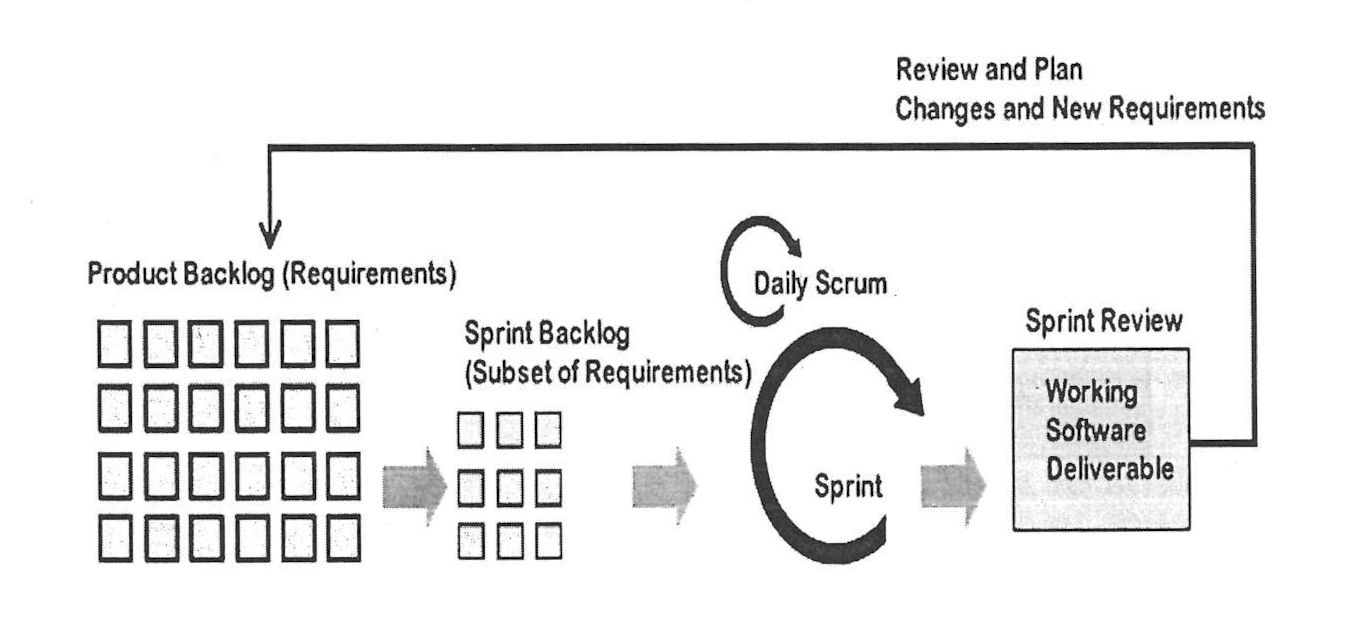
\includegraphics[scale=0.7]{Bilder/Kapitel-2/ScrumProzess.png}
	\caption[Der Scrum-Prozess]{Der Scrum-Prozess \cite[7312]{gut15}}
	\label{fig:scrum_prozess}
\end{figure}

\minisec{Einbezug des Kunden}

Die \textit{Product Owner}-Rolle \marginline{Product Owner}
bei Scrum entspricht im Prinzip der Rolle des Kunden\-vertreters bei XP. Sofern mehrere Kundenvertreter ins Entwicklungsprojekt einbezogen sind, übernimmt einer von ihnen die Product Owner-Rolle. Der Product \mbox{Owner} spezifiziert und priorisiert die Anforderungen an das zu entwickelnde Software\-produkt sowie die zugehörigen Akzeptanztests.

\minisec{Umgang mit Anforderungen}

An Artefakten definiert Scrum neben dem Release nur das sogenannte 
\marginline{Product Backlog, Sprint Backlog}
\textit{Product Backlog} und das \textit{Sprint Backlog}. Das Product Backlog enthält die Anforderungen an das zu erstellende Softwareprodukt. Es wird vom Product Owner erstellt und kontinuierlich ergänzt, verändert und verfeinert, wobei der Product Owner gegebenenfalls von weiteren Domänenexperten oder vom Entwicklungsteam unterstützt wird. Die Verantwortung für das Product Backlog und die Priorisierung der darin enthaltenen Anforderungen (Product Backlog Items genannt) liegt immer beim Product Owner. Über das Product Backlog kann der Product Owner neue Anforderungen jederzeit einbringen, bestehende streichen oder verändern und somit im gesamten Verlauf des Entwicklungsprojekts flexibel Einfluss auf die Entwicklungsrichtung nehmen. 

Das Sprint Backlog enthält diejenigen Anforderungen des Product Backlog, die im aktuellen Sprint umgesetzt werden sollen. Spätestens wenn ein Backlog Item (eine definierte Anforderung) des Product Backlog in das Sprint Backlog aufgenommen wird, müssen Product Owner und Entwicklungsteam eine sogenannte \marginline{Definition of Done}
\textit{Definition of Done (DoD)}  
%\sttpkapitelverweis{Definition of Done}{Kap.~\ref{sec:Kap-x.y}}
für dieses Item erstellen. Eine DoD legt fest, welche Merkmale die Umsetzung einer Anforderung aufweisen muss, damit die Umsetzung als „fertig“ (heißt auslieferbar) gilt. Scrum macht keinerlei Vorgaben, wie eine DoD aussehen muss. Möglich wäre es zum Beispiel, die Erfüllung von bestimmten Akzeptanztests als Kriterium einer DoD anzusetzen.

Zu Beginn jedes Sprints legen Entwicklungsteam und Product Owner im 
\marginline{Sprint Planning} 
\textit{Sprint Planning} gemeinsam fest, welche der vom Product Owner mit höchster Priorität versehenen Product Backlog Items umgesetzt werden können. Spätestens dann müssen die einzelnen Items so detailliert spezifiziert sein (unter anderem durch die DoD), dass eine Aufwandsschätzung möglich ist. Es ist Aufgabe des Scrum Masters während des Sprints diese Aufwandsschätzung kontinuierlich mit dem real geleisteten Aufwand abzugleichen und zu kontrollieren, ob das Sprint-Ziel erreicht werden kann. Unter Umständen muss das Team in Absprache mit dem Product Owner den Leistungsumfang des Sprints reduzieren, indem bestimmte vorgesehene Items nicht umgesetzt werden. Ansonsten sind während eines Sprints keine Änderungen erlaubt. Auch neue Anforderungen, denen der Product Owner eine höhere Priorität zuteilt als den aktuell in der Umsetzung befindlichen, müssen bis zum nächsten Sprint warten, ein Tausch von Items ist nicht möglich. 

Dieses Einfrieren von Anforderungen während eines Sprints ist Scrums Lösung für den Spagat zwischen der Möglichkeit von Anforderungsänderungen und der Notwendigkeit von Planungssicherheit. Für Bertrand Meyer, der für sein 2014 erschienenes Buch „Agile! The Good, the Hype and the Ugly“ \cite{mey14} verschiedene agile Mo\-delle und Methoden analysiert hat, ist diese Scrum-Lösung die bedeutendste Idee des agilen Umfelds.

\vspace{3mm} %%% für Druck

\sttpzitat{„If out of my long immersion in agile methods for the preparation of this book I had to retain just one idea, that would be it. The principle is innovative, applicable, and effective.“ \cite[140]{mey14}}{Betrand Meyer über das Einfrieren von Anforderungen während eines Sprints}

\vspace{3mm} %%% für Druck

Im Kommunikationsformat des \textit{Sprint Review} \marginline{Sprint Review} begutachten und diskutieren Entwicklungsteam, Product Owner und eventuelle weitere Domänenexperten die Ergebnisse des Sprints (Umsetzung der Anforderungen). Daraus resultierende notwendige Änderungen oder neue Anforderungen werden ins Product Backlog eingetragen.

\minisec{Einordnung von Scrum}

Die von Scrum vorgegebenen Elemente sind fast ausschließlich auf der organisatorischen Ebene des Softwarenentwicklungsprojekts angesiedelt. Mit welchen Techniken die Ziele des Sprints erfüllt werden, wie die Aufgabenverteilung im Team aussieht, aber auch, in welcher Art und Weise die vorgegebenen Kommunikationsformate ausgestaltet werden, bleibt dem konkreten Team überlassen. Dieses ist damit in höchstem Maße (im positiven wie im negativen Sinne) eigenverantwortlich. In der Praxis werden insbesondere Teammitglieder, die schon in Scrum-Projekten gearbeitet haben, Ideen zu Prozessabläufen, Entwicklungsmethoden und -werkzeugen beisteuern können.

Wie für XP gilt auch für Scrum, dass es sich erst dann um einen Scrum-Prozess handelt, wenn \textbf{alle} Scrum-Regeln eingehalten werden. Nichtsdestotrotz lassen sich einzelne Scrum-Elemente auch in anderen Modellen verwenden. 

Im Gegensatz zu anderen agilen Modellen gibt es gegenüber Scrum wenige kritische Stimmen. Das hat sicher damit zu tun, dass Scrum keinerlei Vorgaben zu Entwicklungsmethoden macht und insofern, auch im Vergleich zu XP, deutlich weniger radikal wirkt. Theoretisch wäre es sogar möglich, innerhalb eines Sprints in einem wasserfallartigen Vorgehen zu arbeiten oder die einzelnen Product Backlog Items so detailliert schriftlich zu fixieren, dass eine umfassende Dokumentation der Anforderungen inklusive getroffener Entwurfsentscheidungen entsteht. In der Regel wird Scrum aber in Kombination mit agilen Methoden wie Test-First Development und Continuous Integration eingesetzt. Die Herausforderungen bezüglich der Vertragsgestaltung für Auftragsarbeiten und bezüglich vorhandener Unternehmensstrukturen (\zb Controllingabläufe, Berichtspflichten), die auf sequentielle Modelle ausgerichtet sind, teilt Scrum mit anderen agilen Modellen. 

% 2.3
\clearpage
\section{Vorgehensmodelle – Vergangenheit, Gegenwart und Zukunft}
\label{sec:Kap-2.3}

Wir haben uns 
\marginline{(Vor)Urteile}
in diesem Kapitel ausführlich mit Vorgehensmodellen im Softwareengineering befasst. Der eine oder die andere mag irritiert gewesen sein, dass auch die rückständigen sequentiellen Modelle Thema waren, die längst nicht mehr State of the Art sind, bei denen Menschen weniger zählen als Verfahrensabläufe und mit denen der Großteil der Softwareentwicklungsprojekte scheitert. Die eine oder der andere mag dagegen irritiert gewesen sein, dass auch die neumodischen agilen Modelle Thema waren, in denen chaotisch und ohne jegliche Rücksicht auf Budgets wild programmiert wird, die weder Anforderungen erheben noch Software dokumentieren und mit denen Softwareentwicklungsprojekte nie fertig werden.

\vspace{1mm} %%% für Druck

Solche und ähnliche (Vor)Urteile gegenüber der jeweils anderen Art von Vorgehensmodellen führten und führen seit dem Aufkommen der agilen Modelle Ende der 1990er Jahre zu heftigen ideologischen Verwerfungen zwischen Befürwortern und Gegnern agiler Softwareentwicklung. 

%%% Absatz hier für Druck
\vspace{1mm} %%% für Druck

Viele der frühen Verfechter agiler Modelle waren „Enthusiasten“ \cite[108]{som18}, die es als zwingend notwendig erachteten die bestehenden Software\-entwick\-lungs\-verfahren zu verwerfen und im gleichen Atemzug die gesamte Kultur der Soft\-ware\-entwick\-lung zu revolutionieren. Sie waren dementsprechend in keinerlei Hinsicht bereit, ihre agile Version auf bestehende Management\-verfahren und Unternehmens\-kulturen anzupassen oder gar einzuschränken. Die dadurch stark ideologisch geprägte Fundamentalkritik an den bestehenden Vorgehensmodellen erzeugte von deren Befürwortern als Gegenreaktion eine gleicherweise ideologisch geprägte Fundamentalkritik an sämtlichen Verfahrensweisen, die auch nur ansatzweise dem agilen Umfeld zugeordnet werden können. Insbesondere für die Vertreter eines sehr theoretisch orientierten Softwareengineering in Teilen der akademischen Welt (s. S.~\pageref{text:theoVertreter}) waren die agilen Methoden zudem ein ziemlicher Schock, denn sie negierten so ziemlich alles, was zur reinen Lehre der „guten“ Software\-entwicklung gehörte.

\vspace{1mm} %%% für Druck

Von den agilen Vorgehensmodellen war es vor allem XP, das kaum in bestehende Managementverfahren und Unternehmenskulturen passte – auch nicht passen wollte – und dementsprechend Gegenstand heftiger Diskussionen zwischen Befürwortern und Gegnern war. Besonders umstritten war die im Rahmen von XP vorgestellte Methode des Pair Programming, nicht nur aufgrund der offensichtlichen Frage, ob mit Pair Programming mehr oder weniger effizient Programmcode produziert werden kann als mit Einzelprogrammierung, sondern auch wegen der daraus folgenden kollektiven Verantwortung des Entwicklerteams für die Erstellung der Software und die Gewährleistung der Codequalität. Dieser Aspekt war mit den klassischen Vorstellungen von festen Zuständigkeiten und Verantwortlichkeiten einzelner Teammitglieder – insbesondere auch die Übernahme von Verantwortung für begangene Fehler – kaum vereinbar. 

%%% Absatz hier für Druck
\vspace{1mm} %%% für Druck

Es entstand eine Vielzahl von (teilweise wissenschaftlichen, nicht selten aber auch ideologisch angehauchten) Studien zum Pair Programming, allerdings mit so differierenden Ergebnissen, dass sich kein wirklich klares Bild über die Eignung oder Nicht-Eignung bzw. über messbare Vorteile des Pair Programming für die Softwareentwicklung erkennen lässt.\footnote{Wer dieses Thema vertiefen möchte, startet am besten mit den bei \cite[99]{som18} und \cite[232]{boe04} besprochenen Studien zum Pair Programming und nutzt dann deren Literaturangaben für die weitere Studiensuche.} 

\minisec{Bewertungen jenseits von Ideologien}
Es hat seit dem Aufkommen der agilen Modelle und Methoden relativ lange gedauert, bis man begann sich jenseits von ideologischen Betrachtungen der agilen Softwareentwicklung als Heiligem Gral oder achter Todsünde, auch differenzierter mit dem Sinn und Unsinn agiler Softwareentwicklung zu beschäftigen. Eine der ersten Gegenüberstellung von klassischer und agiler Softwareentwicklung lieferten im Jahr 2004 Barry Boehm und Richard Turner mit ihren Buch „Balancing Agility and Disci\-pline“ \cite{boe04}. Der Untertitel „A Guide for the Perplexed“ beschreibt den Fokus des Buchs: die Autoren stellen Kriterien auf, anhand derer konkrete Software\-entwicklungs\-projekte einen für sie gewinnbringenden Mix aus agilem und plangesteuertem – so der im Buch verwendete Begriff für die klassischen Vorgehensweisen – Vorgehen bestimmen können sollen. Anhand verschiedener organisatorischer, struktureller, personeller und technologischer Charakteristika von Softwareprojekten sowie deren Einsatzgebieten identifizieren die Autoren den jeweiligen „Home Ground“ der agilen und der plangesteuerten Softwareentwicklung. Der Begriff \textit{Home Ground} \marginline{Home Ground}
beschreibt dabei die Menge derjenigen Konstellationen von Projektcharakteristika, bei denen der Einsatz des entsprechenden Entwicklungsansatzes im Vergleich zum anderen Ansatz geeigneter ist. Insgesamt plädieren die Autoren aber dafür, nicht im Zustand des „single-method true believers“ \cite[22]{boe04} zu verharren, sondern sich pragmatisch derjenigen plangesteuerten und agilen Methoden zu bedienen, die für das konkrete Softwareentwicklungsprojekt passend erscheinen.

\vspace{3mm} %%% für Druck

\sttpzitat{„For plan-driven methods, that ground is generally large, complex systems, often with safety-critical or other high-reliability attributes. Requirements should be fairly \mbox{stable} and the environment somewhat predictable. Agile methods are more comfortable where the systems and development teams are smaller, the customer and users are readily available, and the requirements and environment are volatile.“ \cite[22]{boe04}}{}

\vspace{3mm} %%% für Druck

Eine analytische Darstellung und Bewertung von konkreten agilen Prinzipien, Rollen und Methoden der wichtigsten agilen Vorgehensmodelle (unter anderem XP und Scrum) lieferte 2014 das von Bertrand Meyer verfasste „Agile! The Good, the \mbox{Hype} and the Ugly“ \cite{mey14}. Sehr offen gegenüber innovativen agilen Konzepten und gleichzeitig sehr kritisch – und teilweise verbal schonungslos – gegenüber manchem Heilsversprechen der agilen Literatur ist dieses Buch die erste systematische wissenschaftliche Darstellung und Bewertung zentraler agiler Methoden und Vorgehensmodelle.

Heutige Lehrbücher zum Softwareengineering gehen recht unterschiedlich mit dem Thema agiler Softwareentwicklung um. Thematisiert wird sie mittlerweile eigentlich immer, aber die Spanne reicht von "`ja, das gibt es auch"' bis zu "`es hat bzw. wird die Softwareentwicklung revolutionieren"'. Ian Sommerville ist einen interessanten Weg gegangen, der auf die Home Ground-Vorstellung von Boehm und Turner passt. Sein Standardlehrbuch \cite{som18} zum Softwareengineering war erstmals 1980 erschienen und dementsprechend auf plangesteuerte Entwicklung ausgerichtet. Im Laufe der mittlerweile zehn Aktualisierungen des Lehrbuchs haben zwar auch agile Methoden ihren Stellenwert im Lehrbuch bekommen. Der rote Faden blieb aber die grundlegende Vorstellung eines von Beginn an systematisch vorgeplanten Softwareentwicklungsprozesses -- auch wenn in der neuesten Auflage die Prozesse des Entwurfs und der Implementierung an vielen Stellen (im Sinne der Vorstellung agiler Entwicklung) als deutlich verzahnte Prozesse dargestellt werden. Parallel erschien aber 2020 Sommervilles weiteres Lehrbuch "`Modernes Software-Engineering"' \cite{som20}, das den Fokus auf die Entwicklung kleinerer und mittlerer (nicht-sicherheitskritischer) Softwareprodukte für den freien Markt setzt. "`Schnelle Entwicklung und Lieferung sowie die Flexibilität, Änderungen schnell vorzunehmen, sind grundlegende Anforderungen an die Produktentwicklung."' \cite[34]{som20} Dementsprechend werden auch viele (ursprünglich) dem agilen Umfeld zugeschriebene Methoden in diesem Lehrbuch vorgestellt. 

\vspace{1mm} %%% für Druck

Die Diskussion, ob agile Softwareentwicklung grundsätzlich sinnvoll ist oder nicht, wird heute nicht mehr ganz so heftig geführt wie in den 1990er und 2000er Jahren, beendet ist sie jedoch nicht. Das hat sicher auch damit zu tun, dass verschiedene Menschen die Agilität oder Nicht-Agilität eines konkreten Software\-entwicklungs\-projekts sehr unterschiedlich bewerten würden. Die Prinzipien des Agilen Manifests sind eben Prinzipien und keine operationalisierbaren Kriterien, anhand derer man den Agilitätsgrad eines konkreten Softwareentwicklungsprojekts eindeutig bestimmen könnte. Andrew Hunt, einer der Autoren des Agilen Manifests hatte zum zehnjährigen Geburtstag des Manifests beschrieben, was Agilität für ihn bedeutet:

\vspace{3mm} %%% für Druck

\sttpzitat{„it’s not about doing pair programming, or having stand-up Scrum meetings. \mbox{Anyone} can dogmatically follow the practices prescribed by others. But true agility goes beyond the dogma, beyond the practices. Agility is about adapting; adapting your process, your language, your tools, your team, and yourself to respond to the situation at hand.” \cite[12]{hun11}}{}

\vspace{4mm} %%% für Druck

\minisec{Eingesetzte Vorgehensmodelle}
\phantomsection
\label{sec:Kap-2.3:heutigeVM}

\vspace{1mm} %%% für Druck

Zahlen zum Einsatz bestimmter (Kategorien von) Vorgehensmodelle(n) sind etwas mit Vorsicht zu behandeln. Manchmal sollen sie zeigen, dass sich ein bestimmtes Vorgehensmodell durchsetzt bzw. nicht durchsetzt. Manchmal wird versucht, ein realistisches Bild zu zeigen, doch ist die vorhandene Datengrundlage so klein, dass sich maximal für genau die befragten Projekte bestimmen lässt, welche Vorgehensmodelle eingesetzt werden. Hinzu kommt, dass auch mit methodischer Sorgfalt bei der Erhebung nicht verhindert werden kann, dass befragte Projekte eine abweichende Vorstellung von der Agilität bzw. Nicht-Agilität ihrer eingesetzten Methoden oder Modelle haben als die befragenden Wissenschaftler. Trotz dieser Einschränkungen möchten wir hier auf die Vorstellung von Zahlen zur Verbreitung von Vorgehens\-modellen nicht komplett verzichten.

Im Rahmen der zweiten Phase der internationalen HELENA\footnote{HELENA: Hybrid dEveLopmENt Approaches in software systems development. Im HELENA-Projekt untersuchen etwa 75 internationale Wissenschaftlerinnen und Wissenschaftler den Einsatz hybrider Methoden in der Softwareentwicklung. Zum Projekt und zugehörigen Publikationen \mbox{s.~\href{https://helenastudy.wordpress.com/}{https://helenastudy.wordpress.com/}}}-Studie \cite{kuh18} wurden Unternehmen gefragt, welche Softwareentwicklungsmodelle und -methoden sie einsetzen (s. Abb.~\ref{fig:softwareentwicklungsmodelle_und_methoden}). Bei den Antworten auf diese Frage finden sich im Jahr 2017 sowohl die agilen Modelle Scrum und XP als auch Wasserfallmodelle und andere Phasenmodelle.

\begin{figure}[h!]
    \centering
    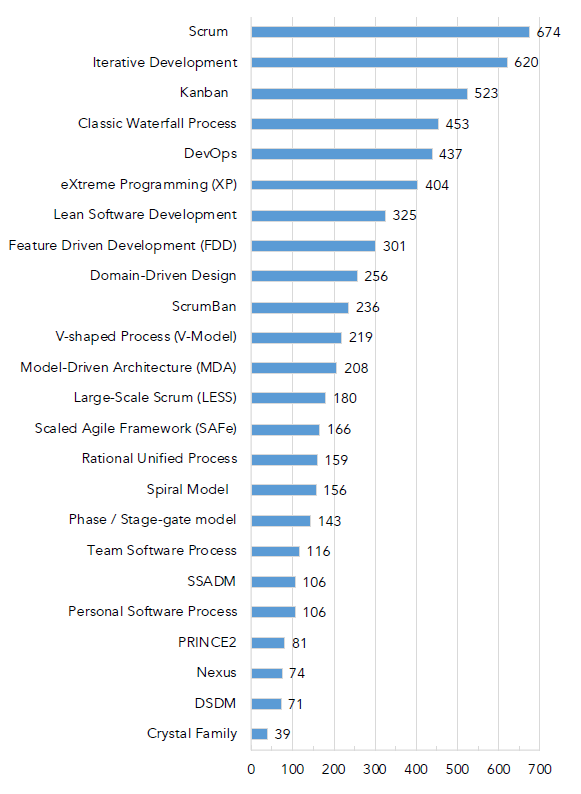
\includegraphics[width=0.7\textwidth]{Bilder/Kapitel-2/VerteilungModelleMethoden.png}
    \caption[Eingesetzte Vorgehensmodelle und Methoden]{Eingesetzte Modelle und Methoden. Mehrfachnennung war möglich. \cite[10]{kuh18}}
    \label{fig:softwareentwicklungsmodelle_und_methoden}
\end{figure}

Die Studienreihe „Status Quo Agile“ der Hochschule Koblenz untersucht regelmäßig den Status Quo der Nutzung agiler Methoden. Für die Studie „Status Quo Agile – 3.~Studie zu Verbreitung und Nutzen agiler Methoden 2016/2017“ \cite{kom17} wurden etwa 1000 Unternehmen aus über 30~Ländern befragt, wobei aber 73\,\% der teilgenommenen Befragten aus Deutschland stammen. 

\pagebreak %%% für Druck

20\,\% der Befragten gaben an nur mit agilen Methoden zu arbeiten (s. Abb.~\ref{fig:einsatz_agiler_methoden}), während 12\,\% nur mit klassischen Methoden arbeiten. Das bedeutet, dass mehr als zwei Drittel der befragten Unternehmen entweder klassische und agile Methoden mixen (Kategorie Hybrid) oder bei einzelnen ausgewählten Prozessen agile Methoden einsetzen (Kategorie Selektiv). In der 4.~Studie der Reihe „Status Quo (Scaled) Agile 2019/20. 4.~Internationale Studie zu Nutzen und Erfolgsfaktoren (skalierter) agiler Ansätze“ \cite{kom20} hat sich im Jahr 2019 an diesem Befund nur wenig verändert. Der Anteil rein klassischer Methoden ist mit 9\,\% der Projekte etwas gesunken, der Anteil der durchgängig agilen Projekte liegt weiterhin bei 20\,\%, die hybriden Projekte konnten mit 43\,\% gegenüber dem nur selektiven Einsatz (28\,\%) etwas zulegen \cite[13]{kom20}.

\begin{figure}[h!]
    \centering
    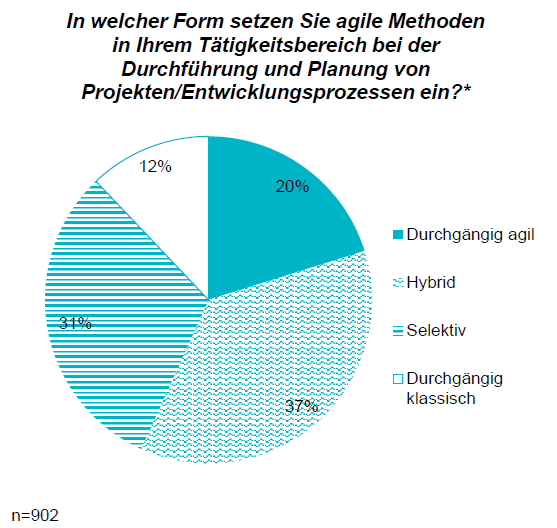
\includegraphics[width=0.7\textwidth]{Bilder/Kapitel-2/EinsatzAgileMethoden.png}
    \caption[Einsatz agiler Methoden bei der Durchführung von Projekten]{Einsatz agiler Methoden bei der Durchführung und Planung von Projekten/Entwicklungsprozessen \cite[15]{kom17}}
    \label{fig:einsatz_agiler_methoden}
\end{figure}

Die Status Quo Agile-Studienreihe hat die Verbreitung agiler Methoden im Blick und fragte daher 2017 auch nach den Gründen, aus denen selektive bzw. hybride Formen – wie aus den vorgegebenen Antwortkategorien hervorgeht: an Stelle komplett agiler Formen – gewählt wurden (Abb.~\ref{fig:gruende_hybrid}). 

%%% Hier kommt Abbildung "fig:gruende_hybrid" eigentlich hin.

Auffällig ist hier, dass anscheinend häufig organisatorische Rahmenbedingungen und institutionelle Zwänge dem reinen agilen Vorgehen im Weg stehen. Vor diesem Hintergrund ist es nicht verwunderlich, dass ein agiles Modell wie Scrum, das deutlich managementfreundlicher als andere agile Modelle ist, sich gegenüber anderen agilen Modellen durchsetzen konnte. In der 4. Studie der Reihe wurde die Frage erneut – allerdings mit etwas abweichenden Antwortkategorien – gestellt \cite[24]{kom20}: Hauptgrund für die Nicht-Wahl eines reinen agilen Ansatzes bleiben die Rahmen\-bedin\-gungen (74\,\%). 

\pagebreak %%% für Druck

\begin{figure}[h!]
	\begin{addmargin*}[0cm]{-\marginparwidth}
		\begin{addmargin*}[0cm]{-\marginparsep}
			\centering
			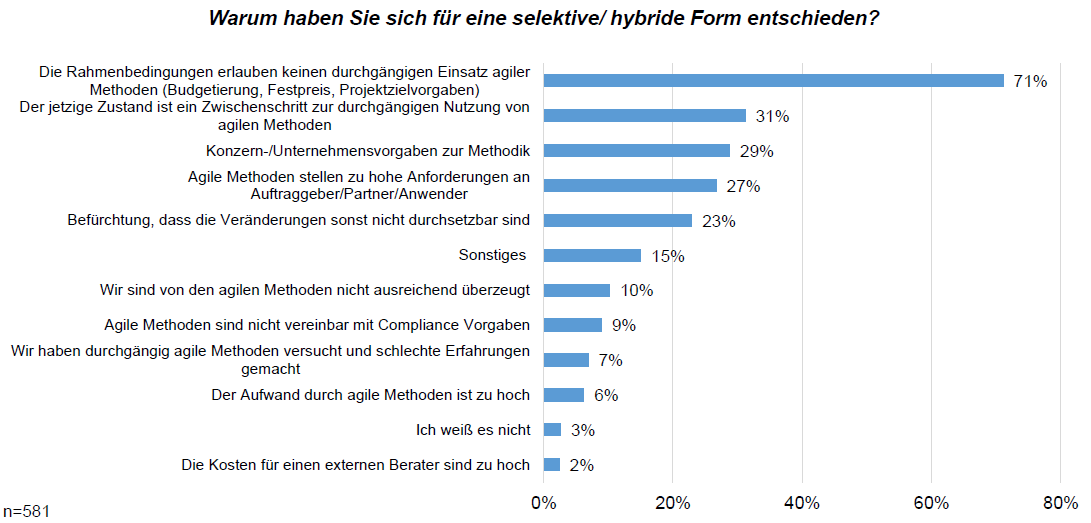
\includegraphics[width=1.25\textwidth]{Bilder/Kapitel-2/GruendeHybrid.png}
			\caption[Gründe für eine selektive/hybride Form]{Gründe für eine selektive/hybride Form. Mehrfachnennung war möglich. \cite[29]{kom17}}
			\label{fig:gruende_hybrid}
		\end{addmargin*}
	\end{addmargin*}
\end{figure}

\begin{figure}[h!]
	\begin{addmargin*}[0cm]{-\marginparwidth}
		\begin{addmargin*}[0cm]{-\marginparsep}
			\centering
			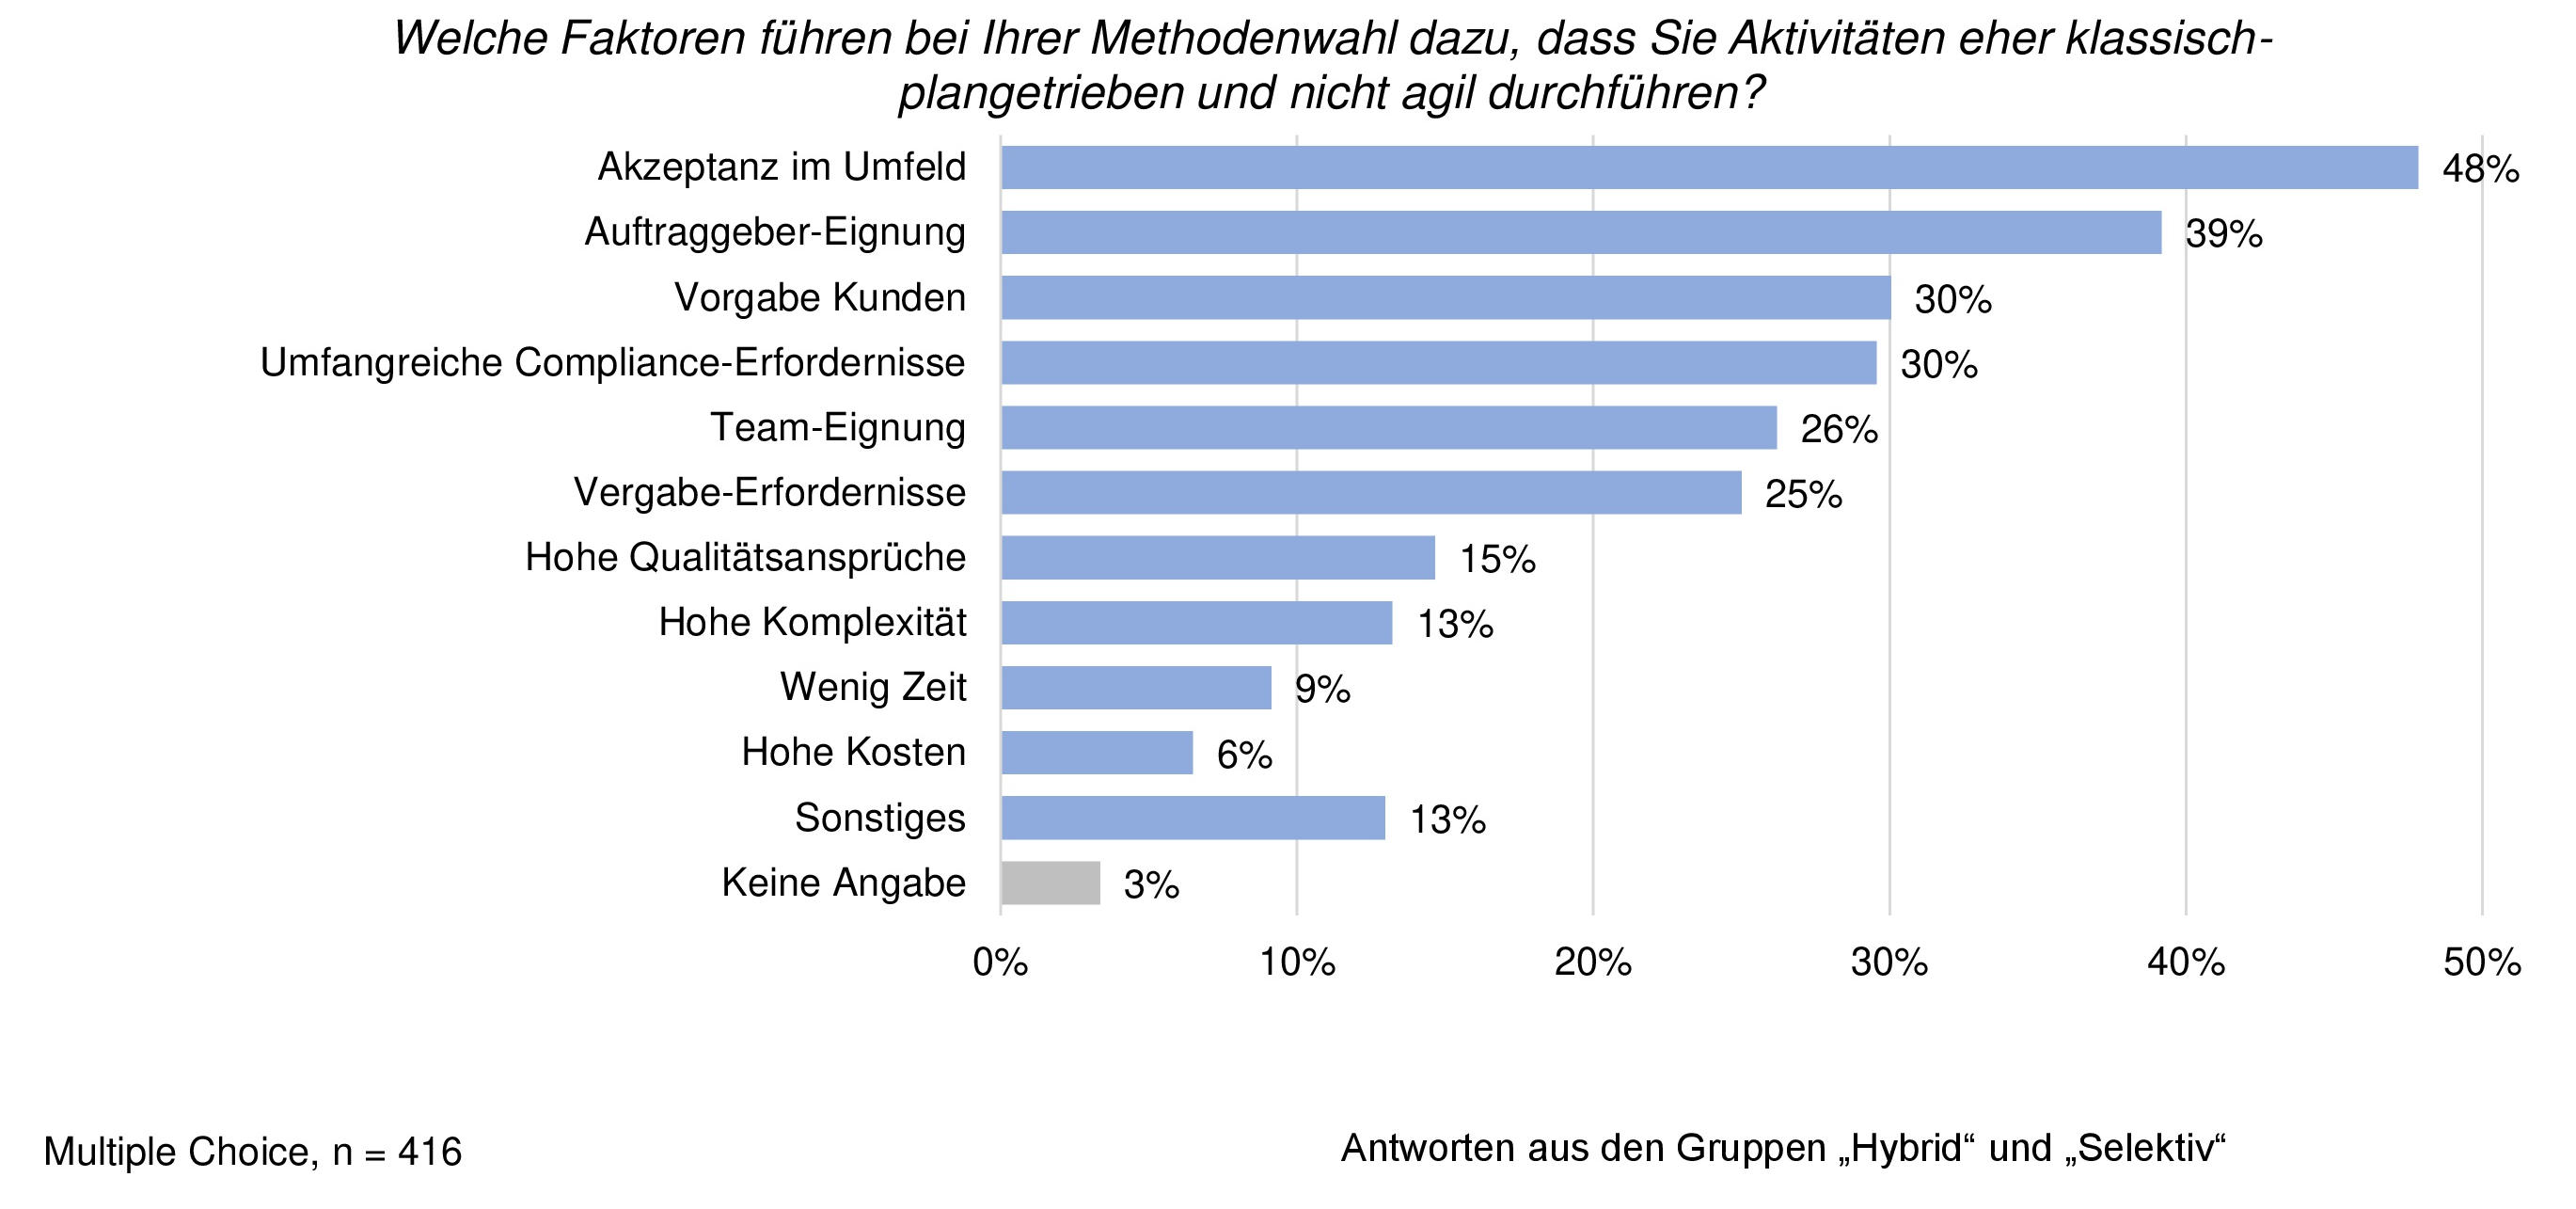
\includegraphics[width=1.25\textwidth]{Bilder/Kapitel-2/GruendeKlassisch.png}
			\caption[Faktoren für die Wahl klassisch-plangetriebener Methoden]{Faktoren für die Wahl klassisch-plangetriebener Methoden. Mehrfachnennung war möglich. \cite[30]{kom20}}
			\label{fig:gruende_klassisch}
		\end{addmargin*}
	\end{addmargin*}
\end{figure}

\pagebreak %%% für Druck

Die 2019er-Studie fragt bei Projekten, die in die Kategorien Hybrid oder Selektiv fallen, außerdem nach den Gründen für die Wahl klassisch-plangetriebener statt agiler Methoden (Abb.~\ref{fig:gruende_klassisch}). Auch hier zeigt sich, dass für die Entscheidung zwischen agilen und plangetriebenen Methoden oft weniger einzelnen Methoden innewohnende Vor- oder Nachteile, sondern vielmehr die verschiedenen Umfeldfaktoren des Softwareentwicklungsprojekts eine Rolle spielen. 

%%% Hier kommt Abbildung "fig:gruende_klassisch" eigentlich hin.

Über Scrum sagen in der 2017er-Studie etwa 55\,\% derjenigen Befragten, die agile Methoden einsetzen, dass es eine zentrale Bedeutung in ihrem Tätigkeitsbereich habe und weitere etwa 25\,\%, dass es neben anderen Methoden in ihrem Tätigkeitsbereich genutzt werde \cite[50]{kom17}\footnote{die Frage lautete: „Welche Bedeutung haben die jeweiligen Methoden für Ihren Bereich?“. Die anderen beiden Antwortkategorien waren „geringe Bedeutung in meinem Tätigkeitsbereich“ und „keine Bedeutung für meinen Tätigkeitsbereich“, siehe \cite[50]{kom17}}. Damit führt Scrum eine Liste von 14 agilen Methoden an, für die die Studie die Bedeutung abfragt. XP liegt mit etwa 10\,\% für „zentrale Bedeutung“ und weiteren 20\,\% für „neben anderen Methoden genutzt“ in dieser Liste auf Platz~6.

Heute werden sie alle irgendwo eingesetzt – die sequentiellen Vorgehensmodelle, die agilen Vorgehensmodelle und vor allem die diversen Ausprägungen dazwischen! Manche Unternehmen versuchen eine gewisse Standardisierung zu erreichen und Projekte nach unternehmenseinheitlichen Vorgehensmodellen durchzuführen. Andere setzen je nach Projekt unterschiedliche Modelle ein. Es ist dabei sehr üblich die Grundform eines Vorgehensmodells spezifisch an das konkrete Projekt oder an übergeordnete Regeln des Unternehmens anzupassen. Die Status Quo Agile-Studie 2017 hat bei Projekten, die Scrum einsetzen, erhoben, inwieweit sich diese von den Vorgaben von Scrum entfernen und auf Grundlage von Scrum ihr eigenes unternehmens\-spezifisches Vorgehensmodell entwickeln: So setzen 11\,\% der Befragten Scrum ohne die Rolle des Scrum Master ein, in weiteren 19\,\% der Projekte agiert der Scrum Master eher wie ein (klassischer) Projektleiter, und 20\,\% der Projekte setzen einen Scrum Master und einen Projektleiter gleichzeitig ein \cite[99]{kom17}. Insofern halten sich nur die Hälfte der befragten Projekte an die in Scrum definierte Rollenausgestaltung des Scrum Master. Ein ähnliches Abweichen vom Grundmodell ist bei der Rolle des Product Owner zu beobachten: 13\,\% der Projekte haben gar keinen Product Owner bzw. lassen die Rolle von einem Mitglied des Entwicklungsteams übernehmen, und in 35\,\% der Projekte definiert der Product Owner die Sprint-Ziele \cite[100]{kom17}, obwohl Scrum hier explizit die gemeinsame Abstimmung zwischen Product Owner und Entwicklungsteam fordert.

\minisec{Fazit}

Sie haben im Laufe des Kapitels verschiedene Kriterien kennengelernt, anhand derer man Vorgehensmodelle unterscheiden kann. Die größten Unterschiede bestehen in den Strategien der Vorgehensmodelle mit neuen oder veränderten Anforderungen umzugehen. Warum ist das so? In einer idealen Welt, in der man für die Entwicklung eines Softwareprodukts unendlich viel Zeit und Geld hätte, alle Anforderungen unmissverständlich benennen könnte und wüsste, dass sich diese Anforderungen niemals ändern würden; in dieser Welt würde man zu Beginn eines Projekts alle Anforderungen detailliert aufschreiben, denn je umfänglicher man zu Beginn über die gewünschte Funktionalität Bescheid weiß, desto zielgerichteter und effizienter kann die Software entwickelt werden. Nur ist das leider unrealistisch. Daher muss jedes konkrete Softwareentwicklungsprojekt in irgendeiner Weise den Spagat schaffen notwendige Änderungen – im Übrigen nicht nur bezogen auf die Anforderungen – im Laufe des Projekts vornehmen zu können und gleichzeitig in der Lage sein das Zeit- und Kostenbudget möglichst einzuhalten, wofür in der Regel die Kontrolle des Projektfortschritts notwendig ist. Die verschiedenen Vorgehensmodelle verfolgen dafür unterschiedliche Strategien. Mit dem flexiblen Reagieren auf Änderungen haben sequentiell orientierte Entwicklungsprojekte die meisten Schwierigkeiten. Die Messung des Projektfortschritts stellt am häufigsten agile Projekte vor Probleme. Es ist daher nicht erstaunlich, dass verschiedene hybride Vorgehensmodelle publiziert werden, die versuchen – und in der Regel auch für sich in Anspruch nehmen es geschafft zu haben – die als sinnvoll erachteten Methoden aus klassischen und agilen Modellen optimal zu vereinen. Mit diesen hybriden Modellen werden wir uns nicht beschäftigen, da uns keines bekannt ist, das aktuell einen größeren Verbreitungsgrad erreicht hätte. Wie auch aus den oben gezeigten Grafiken deutlich wird, gestalten sich Unternehmen oder Projekte sowieso häufig ihre eigenen hybriden Modelle, indem sie zum Beispiel eigentlich agile Modelle um klassische Methoden zum Beispiel zu Projektplanung, Controlling oder Dokumentation erweitern oder in eigentlich sequentielle Modelle agile Elemente zum Beispiel für den Umgang mit Änderungen oder eine andere Art des Testens einbauen.\footnote{\cite{kuh19} werten auf Grundlage der HELENA-Daten \cite{kuh18} hybrides Vorgehen in europäischen Softwareentwicklungsprojekten aus. Der Artikel enthält eine Übersichtstabelle (S.~24~f.) mit Informationen, welche klassischen und welche agilen Methoden von den befragten Projekten kombiniert wurden.}

Ein noch immer heftig diskutiertes Thema im Kontext der Vorgehensmodelle ist die Skalierung von agilen Modellen. Agile Ansätze sind ursprünglich für kleine bis mittlere Teamgrößen gedacht, bei denen die Teammitglieder am selben Ort arbeiten. Diskutiert wird, ob und wie agile Ansätze auch für große und sehr große Entwicklungsteams oder regional verteilt arbeitende Teams sinnvoll eingesetzt werden können. Zu diesem Zweck wurden verschiedene Modelle publiziert. Drei der bekannteren sind das Scaled Agile Framework (SAFe) von Dean Leffingwell, das Agile Scaling Model (ASM) von Scott Ambler und Large-Scale Scrum (LeSS) von Bas Vodde and Craig Larman.\footnote{Weiterführende Informationen zur Skalierung agiler Ansätze und den genannten Modellen bei \cite[104 \psqq]{som18}, \cite[95 \psqq]{kom20} und \cite[41 \psqq]{amb11}.}

Im Umfeld der Vorgehensmodelle auch eher neu (etwa seit den 2010er Jahren) und doch gleichzeitig in gewisser Weise auch sehr alt – weil unter dem Aspekt Wartung schon in manchen sequentiellen Modellen vorhanden – ist die Ausweitung des Blickfelds der Softwareentwicklung in Richtung Softwarebetrieb. Dies ist insbesondere im Rahmen agiler Softwareentwicklung relevant, da Versionen der Software sehr häufig schon produktiv eingesetzt werden, während das Entwicklungsprojekt noch läuft und das Softwareprodukt kontinuierlich weiterentwickelt. Ansätze wie DevOps  
%\sttpkapitelverweis{DevOps}{Kap.~\ref{sec:Kap-x.y}}
betonen daher die Notwendigkeit, Prozesse der Softwareentwicklung und Prozesse des Softwarebetriebs viel enger miteinander zu verknüpfen – auch personaltechnisch. 

Jenseits der Fragen, ob Softwareentwicklung mehr oder weniger Prozesse benötigt, mehr oder weniger Dokumentationen zum Produkt erzeugen muss, sequentieller oder agiler erfolgen sollte; einer der wichtigsten Faktoren für eine erfolgreiche Software\-entwicklung bleibt das Entwicklungsteam. So mag oftmals die Wahl der Methoden und Vorgehensmodelle mehr von der Qualifikation der beteiligten Menschen abhängen als von den Charakteristika des Projekts. Die Vorgehensmodelle sind wichtig und hilfreich, aber mit einem unmotivierten Team entwickelt man mit jedem Vorgehensmodell schlechte Software - oder auch gar keine. Insofern gilt auch heute noch die mehr als dreißig Jahre alte Analyse von Watts Humphrey, der über viele Jahre einer der zentralen Akteure im Bereich der (klassischen) Software\-prozess\-verbesserung war: Es bedarf in jedem Softwareentwicklungsprojekt immer wieder der Abwägung zwischen dem „individual need for flexibility and the organizational need for standards and consistency“. Und dabei ist in jedem Fall zu berücksichtigen: 

\vspace{3mm} %%% für Druck

\sttpzitat{„Since software projects have differences, their software engineering processes must have differences as well. [...] In the absence of a universal software engineering process, organizations and projects must define processes that meet their own unique needs.“ Humphrey 1989, zitiert nach \cite[685]{sha11}}{}

\vspace{3mm} %%% für Druck

Letztendlich muss jedes Softwareentwicklungsprojekt für sich selbst herausfinden, nach welchem Vorgehen die Erstellung qualitativ hochwertiger Softwareprodukte in gegebenen Zeit-, Personal- und Kostenbudgets sowie bei gegebenen Rahmenbedingungen am besten gelingt.

% 2.4
% Kommentierte Literatur beginnt auf neuer Seite
\clearpage
\section{Kommentierte Literatur}
\label{sec:Kap-2.4}

%Bilder/Buchcover/Buchcover_SWEBOK.jpg
\sttpKommLitItem{Bourque/Fairley (Hrsg.)}{2014}{SWEBOK V3.0 – Kapitel 8}{swe14}{}{}
{Kapitel 8 „Software Engineering Process“ des SWEBOK, das Sie schon kennengelernt haben (s. S.~\pageref{sec:Kap-1.4:Bourque}), beschäftigt sich auch mit dem Thema der Vorgehensmodelle. Allerdings werden keine konkreten Vorgehensmodelle vorgestellt, sondern Kategorien von Vorgehensmodellen (sequentiell, inkrementell, iterativ, agil) gebildet und sehr knapp deren wichtigste Unterscheidungsmerkmale thematisiert. SWEBOK nimmt keinerlei Bewertung bezüglich der Überlegenheit oder Unterlegenheit im Vergleich der Vorgehensmodellkategorien vor. Stattdessen wird die Einzigartigkeit von Softwareentwicklungsprojekten und die daraus folgende Notwendigkeit betont, über eine individuelle Auswahl ein passendes Vorgehensmodell einzusetzen. Das Kapitel be\-inhal\-tet zudem Abschnitte zu organisationsbezogenen Softwareentwicklungsprozessen und entsprechenden Reifegradmodellen.}

%Bilder/Buchcover/Buchcover_Sommerville.jpg
\sttpKommLitItem{Sommerville}{2018}{Software Engineering}{som18}{}{}
{Kapitel 2.1 des aus der Einleitung (S.~\pageref{sec:Kap-0.3:Sommerville}) bekannten Lehrbuchs beschäftigt sich mit sequentiellen und in\-kre\-men\-tell-ite\-ra\-ti\-ven Vorgehensmodellen. Das Wasserfallmodell wird ausführlicher dargestellt, für RUP wird auf die Website zum Buch verwiesen. Die agile Softwareentwicklung bekommt in dieser 10. Auflage (engl. Auflage von 2015) ein eigenes Kapitel (Kapitel 3), in dem auch Scrum und XP thematisiert werden. Hervorzuheben sind hier eine gute Kurzzusammenfassung der wichtigsten XP-Praktiken (S. 92 f.) und ein Glossar der Scrum-Begriffe (S. 101) sowie ein eigenes Unterkapitel (Kap. 3.4) zur Skalierung agiler Methoden und der damit verbundenen Probleme. Insgesamt liegt der Schwerpunkt des Kapitels aber bei den heute relevanten agilen Methoden (unabhängig von ihrer Herkunft aus einem bestimmten Vorgehensmodell). Anhand der verschiedenen Auflagen des Lehrbuchs von Ian Sommerville lässt sich der Wandel von relevanten Themen im Softwareengineering beobachten, wie hier am Beispiel der Vorgehensmodelle: In der 9. Auflage des Lehrbuchs von 2011 lag der Schwerpunkt des Kapitels zu agiler Entwicklung noch beim konkreten Vorgehensmodell XP, während die vorhergehende 8. Auflage von 2007 die agile Softwareentwicklung noch gar nicht berücksichtigte, dafür aber ein längeres Unterkapitel zum RUP beinhaltete. Im 2020 erstmals erschienenen anderen Lehrbuch zum Thema Softwareengineering \cite{som20} vom selben Autor erhalten die Methoden der agilen Softwareentwicklung dann nochmal einen höheren Stellenwert.}

%Bilder/Buchcover/zeitung.png
\sttpKommLitItem{Royce}{1970}{Managing the Development of Large Software Systems}{roy70}{}{}
{Der Originalartikel zum ersten Wasserfallmodell [siehe auch Kap.~\ref{sec:Kap-2.2.1.1}]. Kurz und prägnant – zieht man die zahlreichen Abbildungen ab, verbleiben gerade mal \mbox{etwa} viereinhalb Seiten Text – erläutert Royce seine Vorstellung vom strukturierten Ablauf eines Softwareentwicklungsprojekts. Der Stil des Artikels ist sehr handlungsorientiert: viele Aussagen werden in Form von Faustregeln (engl. Howto) formuliert.}

%Bilder/Buchcover/Buchcover_Jacobson_Booch_Rumbaugh.jpg
\sttpKommLitItem{Jacobson/Booch/Rumbaugh}{1999}{The Unified Software Development \\ %%% für Druck
	Process}{jac99}{}{}
{Das Originalbuch zum Unified Process von dessen Erfindern. Der Unified Process verwendet für alle Prozesse als Modellierungssprache die UML, die von denselben Autoren entwickelt wurde. Das Buch stellt dementsprechend bei der Beschreibung der Bestandteile des Unified Process auch die UML vor. Aufbauend auf dem Unified Process sind verschiedene ausdifferenzierte (werkzeugunterstützte) Versionen entstanden, unter anderem der Rational Unified Process [siehe Kap.~\ref{sec:Kap-2.2.2.1} und \cite{kru99}].}

%Bilder/Buchcover/Buchcover_Kruchten.jpg
\sttpKommLitItem{Kruchten}{1999}{Der Rational Unified Process}{kru99}{}{}
{Originalbuch zum Rational Unified Process in deutscher Übersetzung. Das Buch beschreibt detailliert den Rational Unified Process sowie die zugrundeliegenden Best Practices, die der allgemeine Unified Process \cite{jac99} vorgestellt hatte.
}

%{Bilder/Buchcover/Buchcover_Marciniak.jpg}{S. 1804–1806}
\sttpKommLitItem{Alhir}{2002}{Unified Process}{alh02}{}{}
{Überblicksartikel aus einer Enzyklopädie des Softwareengineering zum Rational Unified Process (RUP). Der Artikel stellt den RUP, seine Charakteristika und Besonderheiten auf wenigen Seiten zusammenfassend dar. Er findet damit einen guten Mittelweg zwischen den oft zu verkürzten Darstellungen des RUP in Büchern oder Kapiteln zu Vorgehensmodellen und den vielen, bis ins kleinste Detail gehenden Darstellungen der exklusiv dem RUP gewidmeten Monographien. Der Titel des Artikels ist allerdings irreführend, da er sich nicht mit dem allgemeinen Unified Process, sondern mit der von Rational Software entwickelten Version beschäftigt.}

%Bilder/Buchcover/Buchcover_Beck.jpg
\sttpKommLitItem{Beck}{2003}{Extreme Programming: Das Manifest}{bec03}{}{}
{Die deutsche Übersetzung des Originalbuchs zu Extreme Programming von dessen Erfinder. Das Buch trägt den Untertitel „Das Manifest“ und dementsprechend ist auch die Art der Darstellung. Der Schwerpunkt liegt auf der Beschreibung von Zielen und Philosophie von XP. Die einzelnen Praktiken werden recht allgemein beschrieben oder anhand von einzelnen Anekdoten und Beispielen. Das Buch ist dementsprechend kein Nachschlagewerk, wie genau die Prinzipien von XP in konkreten Projekten angewendet werden können, sondern eher die Beschreibung einer umfassenderen Vision.}

%Bilder/Buchcover/Buchcover_Schwaber_Sutherland.png
\sttpKommLitItem{Schwaber/Sutherland}{2020}{Der Scrum Guide}{sch20}{}{}
{Etwa fünfzehnseitige Darstellung zu Scrums Regeln, Rollen und Artefakten von den Entwicklern von Scrum. Darstellungen zu Scrum findet man heute in zahlreicher Literatur, vielfach sind diese aber uneinheitlich oder sogar widersprüchlich. Da Scrum nur ein Rahmenwerk für agiles Projektmanagement ist und keine eigenen Entwicklungsmethoden (\zb in welcher Form wird getestet?, wie ist das Verhältnis zwischen Programmcode und Dokumentation?) anbietet, wird es in der praktischen Verwendung mit typischerweise agilen Entwicklungsmethoden (\zb Test-First Development) anderer Quellen kombiniert. In der Literatur zu Scrum vermischt sich dadurch häufig die Darstellung der eigentlichen Scrum-Inhalte mit der Darstellung der üblicherweise im Rahmen von Scrum-Projekten verwendeten Methoden. Der Scrum Guide ist das offizielle Scrum-Regelwerk, das bedeutet Regeln, Methoden oder Praktiken, die hier nicht aufgeführt werden, gehören auch nicht zu Scrum. Die Scrum-Autoren sind in dieser Hinsicht etwas puristisch. Sie weisen in einer Schluss\-bemerkung zum Guide zudem daraufhin, dass es sich nicht um eine Scrum-Entwicklung handelt, wenn man nur Teile von Scrum einsetzt. Dies ist, inklusive dem Abändern von Scrum-Regeln, in der Praxis aber durchaus üblich [siehe Kap.~\ref{sec:Kap-2.3}].}

%{Bilder/Buchcover/Buchcover_Gonzalez.jpg}{84-1 bis 84–28}
\sttpKommLitItem{Favaro}{2014}{Agile}{fav14}{}{}
{Dieser Artikel aus dem Softwareengineering-Handbuch \cite{gon14} stellt die Prinzipien des Agilen Manifests, daraus resultierende agile Methoden der Softwareentwicklung sowie konkrete agile Modelle – unter anderem XP und Scrum – vor. Unter einem recht weiten Blickwinkel werden dabei sowohl Vorläufer und Entstehungshintergrund einzelner Methoden, Gründe und Anlässe für ihre Aufnahme in den agilen Methodenkanon als auch die Konsequenzen ihres Einsatzes für die konkrete Ausgestaltung von Softwareentwicklungsprojekten dargestellt. Zudem stellt der Autor vor, welchen Weg – auch in nicht-agile Ansätze – die verschiedenen Methoden in der Softwareentwicklung seit der Veröffentlichung des Agilen Manifests genommen haben. Im zweiten Teil des Artikels gibt der Autor einen zusammenfassenden Überblick über Themen und Ergebnisse aktueller (2014) Forschungsfelder im agilen Umfeld. Der Artikel schließt mit einer umfangreichen Literaturliste und ist als Einstieg für die weitergehende Beschäftigung mit agilen Methoden und Modellen sehr zu empfehlen.}

\sttpKommLitItem{Sommerville}{2020}{Modernes Software-Engineering}{som20}{}{}
{Dieses Lehrbuch steht parallel zu dem regelmäßig aktualisiertem Standardlehrbuch zum Softwareengineering  \cite{som18} des Autors. Es verfolgt einen anderen Ansatz und setzt einen produktbezogenen anstelle eines projektbezogenen Fokus. Insbesondere geht es dabei mehr von Softwareentwicklungen für den Verkauf aus und weniger von einem Kunden, der eine Spezifikation vorgibt, aufgrund derer eine Softwarefirma ihm in einem Entwicklungsprojekt eine maßgeschneiderte Software erstellt. Das Buch beschäftigt sich sehr ausführlich mit agiler Softwareentwicklung und ihren wichtigsten Methoden.}

%{Bilder/Buchcover/Buchcover_Laplante.jpg}{S. 29–46}
\sttpKommLitItem{Ambler}{2011}{Agile Software Development}{amb11}{}{}
{Ein deutlich pro-agil gefärbter – der Autor ist ein überzeugter Vertreter und Entwickler agiler Methoden – aber nichtsdestotrotz sehr informativer Artikel über agile Softwareentwicklung. Der Artikel stellt verschiedene agile Praktiken vor und beschreibt, worin sich agile Ansätze von klassischen Softwareentwicklungsansätzen unterscheiden und worin sich beide Arten ähneln. Zielgruppe sind Projekte, die von anderen Vorgehensmodellen auf agile Vorgehensweisen wechseln möchten. Dafür beschäftigt sich der Artikel auch mit der Skalierung agiler Ansätze, die in der Regel für kleine und mittlere Teamgrößen konzipiert wurden, auf große und sehr große Entwicklungsteams.}

%/Bilder/Buchcover/Buchcover_Cockburn.jpg
\sttpKommLitItem{Cockburn}{2003}{Agile Software-Entwicklung}{coc03}{}{}
{Der Autor gehört zu den Begründern des Agilen Manifests und hat mit den sogenannten Chrystal-Family-Methoden auch selber ein agiles Vorgehensmodell vorgelegt, das in einem Kapitel dieses Buchs thematisiert wird. Der Schwerpunkt des Buchs liegt aber auf einer allgemeineren Beschreibung von Zielen, Philosophie und Methodik agiler Softwareentwicklung, insbesondere in den Bereichen Stellenwert von Individualität im Entwicklungsteam und Kommunikation. Ähnlich wie im Buch von Beck über XP \cite{bec03} geht es hier um die Darstellung einer Vision und weniger um Faktenwissen zu agilen Methoden. Sehr lesenswert ist das Kapitel über das Agile Manifest (S. 281ff), in dem aus einer Beteiligtenperspektive über Gründe und Zufälle für das Entstehen der Werte und Prinzipien des Manifests referiert wird.}

%/Bilder/Buchcover/zeitung.png
\sttpKommLitItem{Kneuper}{2017}{Sixty Years of Software Development Life Cycle Models}{kne17}{}{}
{Der Zeitschriftenartikel beschäftigt sich mit der Geschichte der Vorgehensmodelle seit den 1950er Jahren und stellt dabei auch die Verbindungen zwischen den Modellen (welches Modell ist aus welchem hervorgegangen) dar. Von den hier im Text betrachteten Vorgehensmodellen werden das Wasserfallmodell von Royce und der Rational Unified Process ausführlicher betrachtet. Die agilen Modelle werden nur allgemein behandelt. Dafür berücksichtigt der Artikel auch die frühen Modelle der 1950er und 1960er Jahre und stellt zum Beispiel das Modell von Benington, das wir im Zusammenhang mit dem Wasserfallmodell nur kurz erwähnt haben, detaillierter vor.}

%Bilder/Buchcover/Buchcover_Balzert.jpg
\sttpKommLitItem{Balzert}{2008}{Softwaremanagement}{bal08}{}{}
{Der dritte Band des dreibändigen Lehrbuchs zur Softwaretechnik beschäftigt sich mit Themen des Softwaremanagements. Einen großen Raum nimmt dabei der Abschnitt zu Vorgehensmodellen (unter dem Begriff Prozessmodell), Qualitätsmodellen und Reifegradmodellen ein (Kap. 16-24). Die Kategorisierung der Vorgehensmodelle unterscheidet sich von derjenigen von SWEBOK \cite{swe14}, die uns als Grundlage diente. Die hier im Text behandelten Vorgehensmodelle finden sich aber alle auch bei Balzert – entsprechend seiner Kategorisierung verteilt über verschiedene Kapitel.}

\sttpKommLitItem{Studienreihe Status Quo Agil – 3. Studie}{2017}{}{kom17}{}{}
{\href{https://www.gpm-ipma.de/wissen/studien/status-quo-agile}{https://www.gpm-ipma.de/wissen/studien/status-quo-agile}

Die Studienreihe „Status Quo Agile“ [siehe auch Kap.~\ref{sec:Kap-2.3}], wird vom „BPM-Labor für Business Process Management und Organizational Excellence“ der Hochschule Koblenz in Zusammenarbeit mit Scrum.org, GPM Deutsche Gesellschaft für Projektmanagement e.V. und teilweise weiteren wechselnden Partnern durchgeführt. Die Studienreihe erfragt seit 2012 alle paar Jahre in einer nicht-repräsentativen Studie die Nutzung agiler Methoden in Unternehmen. Schwerpunktmäßig werden Projekte der Softwareentwicklung oder anderer IT-naher Bereiche befragt, es finden sich aber auch Angaben aus IT-fernen Projekten. Etwa dreiviertel der Studienteilnehmer sind deutsche Unternehmen. Die einzelnen Studien der Reihe legen unterschiedliche Schwerpunkte, ein Großteil der Fragen bleibt aber ähnlich (teilweise veränderte Antwortkategorien).}

\sttpKommLitItem{Studienreihe Status Quo Agil – 4. Studie}{2019/20}{}{kom20}{}{}
{\href{https://www.gpm-ipma.de/wissen/studien/status-quo-agile}{https://www.gpm-ipma.de/wissen/studien/status-quo-agile}

Die Studie von 2020 setzt einen inhaltlichen Schwerpunkt auf den Themenbereich Skalierung agiler Ansätze  \cite[95 \psqq]{kom20}.}

%Bilder/Buchcover/zeitung.png
\sttpKommLitItem{Hunt et al.}{2011}{Agile @ 10}{hun11}{}{}
{Anlässlich des 10. Geburtstages des Agilen Manifests 2011 sendeten zehn der siebzehn Urheber ihre Gedanken zu den Fortschritten und Herausforderungen der agilen Softwareentwicklung für einen kurzen Zeitschriftenartikel einer Onlinezeitschrift ein. Die Beiträge der Autoren sind unterschiedlich lang und meist im Stil einer Kolumne gehalten. Sie beschreiben pointiert und sehr unterschiedlich enthusiastisch den Stellenwert der agilen Methoden innerhalb der Softwareentwicklung zehn Jahre nach der Veröffentlichung des Agilen Manifests.}

%Bilder/Buchcover/Buchcover_Boehm_Turner.jpg
\sttpKommLitItem{Boehm/Turner}{2004}{Balancing Agility and Discipline}{boe04}{}{}
{Eine sehr gute Gegenüberstellung zwischen plangesteuerter und agiler Softwareentwicklung bezüglich deren Charakteristika, Stärken und Schwächen, geeigneten Einsatzgebieten etc. [siehe auch Kap.~\ref{sec:Kap-2.3}]. Darüber hinaus werden ausführliche Fallbeispiele aus der Praxis vorgestellt, die die Grenzen von rein plangesteuertem und rein agilem Vorgehen aufzeigen sollen. In diesem Kontext sehr nett zu lesen ist auch die – natürlich entsprechend konstruierte – Fabel von Elefant (plangesteuerte Modelle) und Affe (agile Modelle), mit der die Autoren ihr Buch beginnen und die ihr Credo beinhaltet: Elefant und Affe sind erst dann erfolgreich, wenn sie die Stärken des jeweils anderen anerkennen und einen Weg gefunden haben, ihre Stärken zu verbinden. Die Autoren Barry Boehm (Wasserfallmodell, Spiralmodell) und Richard Turner (Reifegradmodell CMMI) verband man zur Entstehungszeit des Buchs (2004) eher mit plangesteuerter als mit agiler Softwareentwicklung. Die von Pragmatismus statt von Ideologie geleitete Herangehensweise der Autoren zeigt sich auch daran, dass Alistair Cockburn (einer der Autoren des Agilen Manifests) ein sehr positives Vorwort zum Buch verfasst hat.}

%Bilder/Buchcover/Buchcover_Meyer.jpg
\sttpKommLitItem{Meyer}{2014}{Agile! The Good, the Hype and the Ugly}{mey14}{}{}
{Der Autor Bertrand Meyer gehört zu den Großen in der Informatik: er hat wichtige Prinzipien der objektorientierten Softwareentwicklung entworfen, die Programmiersprache Eiffel erfunden und das in der Softwareentwicklung wichtige Konzept „Design by Contract“ entwickelt. Im Umfeld der agilen Softwareentwicklung war er bis zu diesem Buch weniger präsent. Das Buch stellt agile Prinzipien, Rollen und Methoden (unter anderem diejenigen von XP und Scrum) vor und bewertet sie hinsichtlich ihrer Vor- und Nachteile, ihrer Eignung für die praktische Softwareentwicklung und ihres Innovationspotenzials. Der Schwerpunkt des Buchs liegt auf der Bewertung der agilen Ansätze [siehe auch Kap.~\ref{sec:Kap-2.3}]. Die dafür notwendige Beschreibung der Ansätze ist in der Darstellungsart dabei teilweise stringenter und verständlicher als in vieler agiler Originalliteratur.}